\documentclass[12pt,a4paper]{article}
\usepackage{graphicx}
\usepackage{minted}
\usepackage{float}
\usepackage{multicol}
\usepackage{multirow}
\usepackage[english, magyar]{babel}
\usepackage{hyperref}
\usepackage{comment}
\usepackage{ragged2e}
\usepackage[backend=biber,style=numeric]{biblatex}
\usepackage{amsmath}
\usepackage{titling}
\usepackage{bookmark}
\usepackage{t1enc}
\usepackage{csquotes}
\usepackage{subcaption}
\usepackage[margin=20mm]{geometry}
\usepackage{booktabs}
\usepackage{pdfpages}
\usepackage{setspace}

\setlength{\parindent}{1cm}

\onehalfspacing

\hypersetup{
    colorlinks=true,
    linkcolor=black,
    filecolor=magenta,
    urlcolor=cyan
}

\newcommand{\firstpage}{
\thispagestyle{empty}
\vspace*{5mm}
\begin{center}
    {\Large Széchenyi István Egyetem\\}
    {\Large Gépészmérnöki, Informatikai és Villamosmérnöki Kar}
\end{center}
\vspace{35mm}
\begin{center}
    {\huge \bf SZAKDOLGOZAT}
\end{center}
\vspace{35mm}
\begin{center}
    {\huge Péter Bence Gábor}
\end{center}
\vspace{3mm}
\begin{center}
   {\LARGE Mérnök informatikus BSc szak}
\end{center}
\vspace{35mm}
\begin{center}
   {\LARGE 2023}
\end{center}
{\small A gerincen:}\newline
\noindent\framebox[16cm]{Péter Bence Gábor\ 2023\ Nyilvános\ \hfill}
\newpage
}


\bibstyle{ieeetr}
% \bibliography{biblio.bib}
\addbibresource{biblio.bib}

\sloppy

\begin{document}

\firstpage{}

\begin{titlepage}
    \begin{center}
        \vspace*{1mm}
        \begin{tabular}{cc}
            \multirow{4}{*}
             & {\includegraphics*[width=0.6\columnwidth]{sze_givk_logo.png}} \tabularnewline
             & {\huge{}Széchenyi István Egyetem}\tabularnewline
             & {\huge{}Gépészmérnöki, Informatikai}\tabularnewline
             & {\huge{}és Villamosmérnöki Kar}\tabularnewline
        \end{tabular}
        \vspace{10mm}
        \begin{center}
            {\huge \bf SZAKDOLGOZAT}
        \end{center}
        \vspace{10mm}
        \begin{center}
            % {\huge \bf Gépi látás és gépi tanulás alapú közlekedési csomópont elemzés}
            {\huge \bf Járművek trajektóriáinak előrejelzése machine learning modellekkel}
        \end{center}
        \vspace{10mm}
        \begin{center}
            {\huge Péter Bence Gábor\\Témavezető:\\Dr. CSc Horváth András}
        \end{center}
        \vspace{10mm}
        \begin{center}
            {\LARGE Mérnök informatikus BSc szak}
        \end{center}
        \vspace{10mm}
        \begin{center}
            {\LARGE Győr, 2023}
        \end{center}
    \end{center}
\end{titlepage}
\newpage

% feladatkiiro lap
\includepdf[pages={1}]{PeterBenceGaborFeladatKiiroLap.pdf}

% hallgatoi nyilatkozat
\includepdf[pages={1}]{hallgatoinyilatkozat_pbg.pdf}

\newpage

\tableofcontents
\newpage
\listoffigures
\newpage
\listoftables

\newpage
\renewcommand{\abstractname}{}
\begin{abstract}
    \noindent \begin{center}\textbf{Kivonat}\end{center} \par
    \vspace{10pt}
    \paragraph{Az ITS (intelligent transportation system)} egyre nagyobb teret hódít napjainkban és rengeteg különböző területen alkalmazzák ezeket a rendszereket. A közlekedési csomópontok elemzése egy frekventált terület az ITS alkalmazásokban.
    \paragraph{Célunk} gépi látás és gépi tanulás felhasználásával, közlekedési csomópontok elemzésének automatizálása és felgyorsítása. A kutatás eredményeit, a kifejlesztett keretrendszert és a felmerülő problémák megoldásait a gyakorlatban balesetek megelőzésére, renitens viselkedések kiszűrésére és forgalomirányító rendszerek támogatására lehet használni. 
    A kutatásban egy trajektória osztályozó módszert ismertetünk, amely objektum detektálás és objektumkövetés segítségével elemezze a közlekedési csomópontokban elhaladó járművek mozgását. 
    A mozgásuk alapján klaszterezi a trajektóriákat. A klaszterező algoritmus paramétereinek változtatásával különböző finomságú útvonal szétválasztás érhető el. Ezek az útvonal csoportok bemenetként szolgálnak az osztályozó algoritmus tanításánál, ami betanítás után valós időben tudja prediktálni a belépő járművek kimeneti pontjait. 
    \paragraph{OPTICS} klaszterező algoritmus bizonyult a mi esetünkben a leghatásosabbnak. Az OPTICS által csoportosított útvonalak végpontjai alapján további finomításra van lehetőség egy általunk létrehozott algoritmus segítségével, ami a KMeans algoritmust használja fel alapul. 
    \paragraph{Osztályozás} A közlekedők útvonalainak valós idejű előrejelzésére létrehozott módszerekben az SVM, KNN és DecisionTree osztályozó algoritmusok érték el a legmagasabb pontosságot az általunk végzett kiértékelések során. Ez számszerűen 90\% feletti átlagos pontosságot jelentett.
    \paragraph{Grafikus felület} fejlesztésével valós idejű előrejelzéseket tudjuk vizualizálni, ami egy prototípusnak is szolgál a későbbi fejlesztésekhez, amik a gyakorlatban való alkalmazást célozzák meg.
    \paragraph{Továbbá} az általunk kifejlesztett keretrendszer alkalmas forgalomszámlálásra és forgalmi statisztikák előállítására, ami értékes információként szolgálhat közlekedésmérnököknek.
    Ezeket a forgalmi statisztikákat hisztogramok, hőtérképek és idősorok formájában készítettük el. 
    Az adathalmaz kialakításáról, elemzési módszereiről témavezetőmmel egy közlekedési és mobilitási folyóiratban publikáltunk cikket \cite{aggpeterhorvath2023}.
\end{abstract}

\newpage
\renewcommand{\abstractname}{}
\begin{abstract}
    \noindent \begin{center}\textbf{Abstract}\end{center} \par
    \vspace{10pt}
    \paragraph{Intelligent transportation systems (ITS)} are increasingly gaining importance nowadays, and they are being applied in various fields. Traffic node analysis is a popular topic in ITS applications. 
    \paragraph{Our goal} is to automate and accelerate traffic node analysis using machine vision and machine learning techniques. 
    \paragraph{The research results}, developed framework, and solutions to emerging problems can be used in practice to prevent accidents, detect aggressive driving, and support traffic management systems. 
    \paragraph{We introduce} a trajectory classification method that analyzes the movement of vehicles passing through traffic nodes using object detection and tracking. The algorithm clusters the trajectories based on their motion patterns. By adjusting the parameters of the clustering algorithm, we can achieve different levels of route separation. These routes serve as input to the classifier algorithm, which predicts the output points of incoming vehicles in real-time after training. 
    \paragraph{OPTICS} clustering algorithm proved to be the most effective in our case. Using the endpoint of the routes clustered by OPTICS, we can further refine the classification with an algorithm we developed that uses the KMeans algorithm as a foundation. 
    \paragraph{The classifcation methods} we developed for real-time prediction of traffic routes achieved the highest accuracy in our evaluations, using the SVM, KNN, and Decision Tree classification algorithms. This means an average accuracy of over 90\%.
    \paragraph{Graphical interface} development allows us to visualize real-time predictions, which also serves as a prototype for future developments aimed at practical application.
    \paragraph{Additionally} our developed framework is suitable for traffic counting and generating traffic statistics, providing valuable information for transportation engineers.
    These traffic statistics were created in the form of histograms, heat maps, and time series.
    We published an article with my supervisor on the development of the dataset and the analysis methods in a journal of transportation and mobility \cite{aggpeterhorvath2023}.

\end{abstract}

\newpage

\section{Bevezetés}
A nagy számú jármű, útvonal és csomópont miatt az is nagy kihívás, hogy számszerű és pontos képet kapjunk
a közlekedés dinamikájáról, az egyes útvonalak leterheltségéről és a közleketők útvonalválasztási szokásairól.
Ennek követésére számtalan tradicionális módszer is létezik (pl. ember által végzett forgalom-számlálás).
Dolgozatomban egy olyan módszert mmutatok be, mely erre a kérdésre a már fentlevő forgalomfigyelő
kamerák képének elemzésével pontos, részletes eredményeket ad.
\paragraph{Az ITS (intelligent transportation system)} fejlesztése a városokban erre megoldást jelenthet. Ez magában foglalja az információs és
kommunikációs technológiák, mint pélául szenzorok, kamerák, kommunikációs hálózatok és adatelemzés fejlesztését. 5G hálózatokon
keresztül ezek a technológiák összeköthetők a közlekedési eszközökkel. Ehhez okos forgalomirányítási rendszerek kifejlesztésére
van szükség, amik információval tudnak szolgáni a járművekbe szerelt informatikai rendszereknek.
\paragraph{A legértékesebb információt} a közlekedésben részvevő járművek jelen és jövőbeli pozíciója jelenti. Pontos és gyors trajektória
előrejelző rendszerek kifejlesztése nagy kihívás és egyre növekszik irántuk a kereslet. E kutatási terület kiforratlanságából
eredően, kevés létező keretrendszer és adathalmaz található, így a tanító adathalmaz gyűjtése, adatok kinyerésének formátuma, tárolása
és mérőszámok kifejlesztése (amivel a tesztelni kívánt modellek pontosságát tudjuk mérni) is a kutatáshoz tartoznak.
Ebben a kutatásban erre a problémára törekszünk egy módszertant és keretrendszert kifejleszteni, emellett klaszterezési és klasszifikációs
gépi tanulási algoritmusokat tesztelni.
\paragraph{Machine Learning} A gépi tanulás számos különböző típusa létezik, például a felügyelt tanulás, a felügyelet nélküli tanulás és a megerősítő tanulás. 
\paragraph{A felügyelt tanulásban} a modell az adatokon keresztül próbál megtanulni egy adott feladatot. A modellnek az adatok mellett ismert kimeneti értékekre van szüksége, amelyek segítik a modell tanulását és az előrejelzéseket. 
\paragraph{A felügyelet nélküli tanulásban} a modellnek az adatokból kell megtalálnia a mintákat és összefüggéseket anélkül, hogy előzetesen ismert kimeneti értékekre támaszkodna. 
\paragraph{A megerősítő tanulásban} a modell az adatokon és a rendszeren keresztül próbál megtanulni, és visszajelzést kap a teljesítményéről.
\paragraph{A gépi tanulás nagyon széles körben alkalmazható} például az automatikus beszédfelismerésben, a képfelismerésben, a termékajánlásokban, a pénzügyi előrejelzésekben, az egészségügyben és az üzleti elemzésekben. Az adatok rendelkezésre állása miatt az iparágak és a kutatási területek számos területen használják a gépi tanulást az előrejelzések és a döntéshozatal támogatása érdekében.
\paragraph{Mi esetünkben} forgalomban résztvevő objektumok trajektóriájának osztályozáshoz használjuk ezeket a gépi tanulási algoritmusokat.
A forgalomban fellelhető szabályosságokat, unsupervised tanulási módszerrel, úgynevezett klaszterezéssel határozzuk meg. Erre a feladatra KMeans, BIRCH \cite{10.1145/233269.233324} és DBSCAN \cite{10.5555/3001460.3001507}\cite{10.1145/3068335}, OPTICS \cite{10.1145/304181.304187} algoritmusokat teszteltük.
\paragraph{A klaszterezés} során az objektumok be- és kimeneti pontjai szolgálnak bemenetként az algoritmusoknak, az algoritmusok által meghatározott trajektória klaszterek lesznek a klasszifikáció tanításására felhasznált osztályok.
A klaszterezési lépés felgyorsítja a klasszifikációs modellek tanítását, mivel a trajektóriák osztályokba sorolását kézzel is el lehetne végezni, ami nagy adathalmazok esetén nagyon hoszzú idő lenne.
\paragraph{Az osztályozás} egy supervised tanulási módszer, amihez mi bináris klasszifikációs modelleket kombinálunk, ami magas osztályszámnál, ami a mi esetünkben átlagosan 10-15 között volt, igen hatékony. Minden bináris modellnél, egy osztály az összes többivel szemben van betanítva. A modellek pontosságának kiértékelésére 3 mérőszámot alkalmaztunk, amik az \emph{Accuracy Score}, \emph{Balanced Accuracy Score} \cite{10.1109/ICPR.2010.764} és \emph{Top-k Accuracy Score}.
Mindegyik mérőszám kiszámolásához \emph{K-Fold Cross-Validation} \cite{Anguita2012TheI} metódust alkalmaztunk, ahol \begin{math}K=5\end{math}.

% \begin{figure}
%     \centering
%     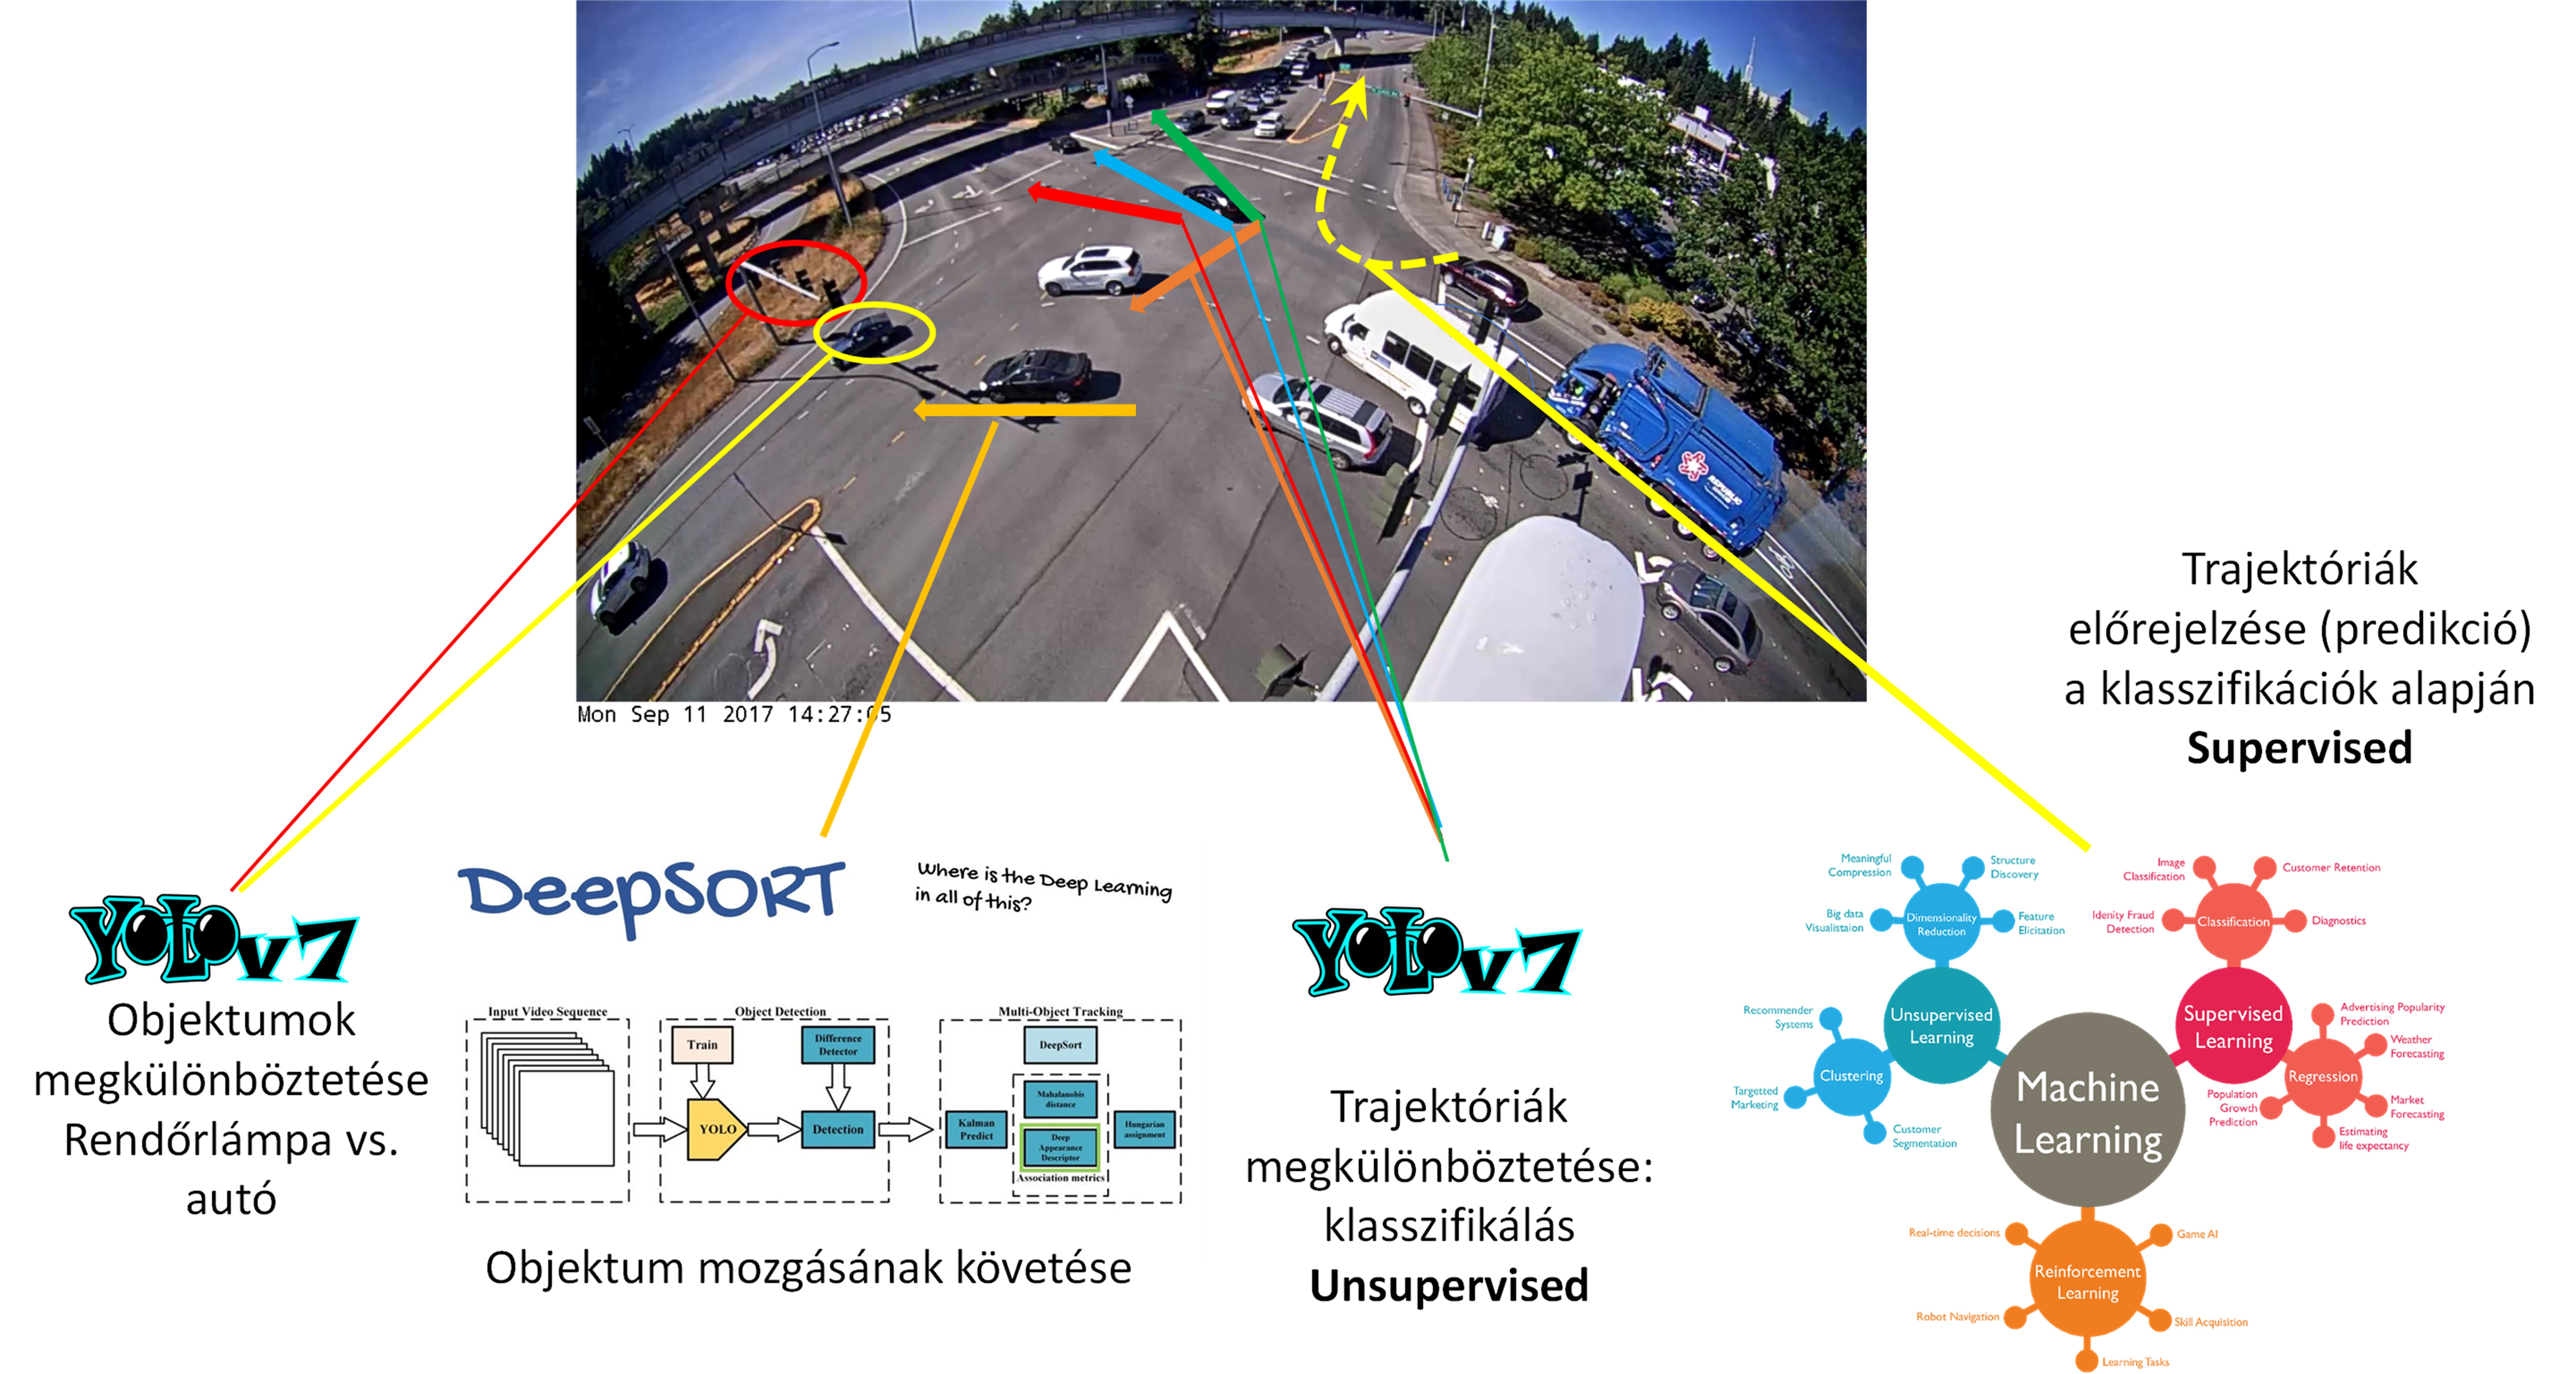
\includegraphics[width=1\columnwidth]{deepsort_yolo_figs/gépilátás_modified.jpg}
%     \caption{Gépi látás}
%     \label{fig: ComputeVision}
% \end{figure}

\paragraph{A tanító adatok} előállításához, objektumok detektálására a YOLOv7 \cite{wang2022yolov7} konvolúciós neurális hálót használtuk, ez a konvolúciós neurális háló architektúra nem csak nagy pontosságot, hanem sebességet is nyújt nekünk.
Emellett képkockáról képkockára követni is kell tudni a detektált objektumokat. Erre is sok megoldás található manapság, erre a feladatra
a DeepSORT \cite{Wojke2018deep} nevezetű algoritmust használtuk, ez Kálmán-filtert és konvolúciós neurális hálót használ az objektumok követésére.
\paragraph{A tanító adatok} 5 különböző helyszín forgalmát tartalmazzák. Minden helyszín más tulajdonságokkal bír, ezért nem lehet generalizálni
a tanítási folyamatot, nem lehet egy univerzális modellt betanítani ami minden közlekedési helyszínre alkalmazható egyaránt.
4 videót Bellevue város github oldaláról gyűjtöttük, amiknek az elérhetőségét függelékként csatoljuk, a kereszteződések
\ref{fig: BellevueNewport}. \ref{fig: BellevueEastgate}. \ref{fig: BellevueNE}. \ref{fig: BellevueSE}. képeken láthatók, az ötödik videó La Grange-ból származik lásd \ref{lagrangekynorth}. A videók pontos elérhetőségét
a mellékletben található \emph{urls.txt}-ben adtuk meg.
\begin{figure}
    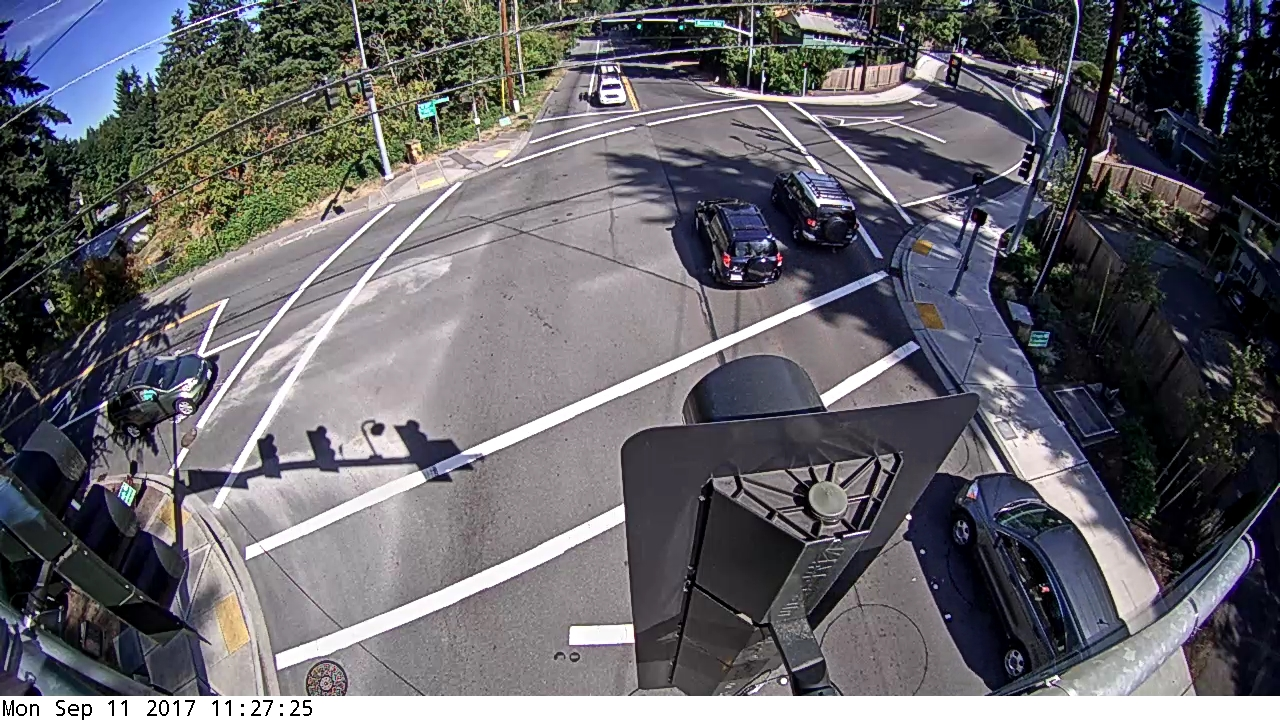
\includegraphics[width=1\columnwidth]{dataset_samples/Bellevue_150th_Newport.JPG}
    \caption{Bellevue Newport kereszteződés}
    \label{fig: BellevueNewport}
\end{figure}
\begin{figure}
    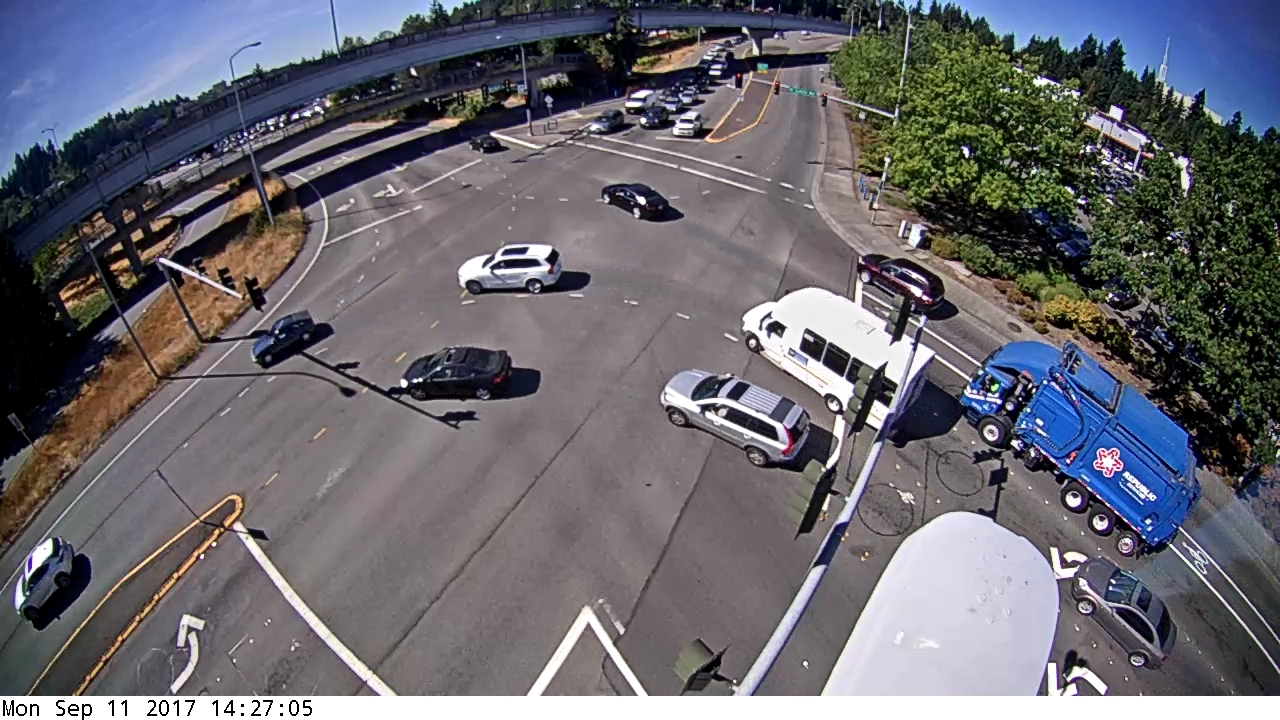
\includegraphics[width=1\columnwidth]{dataset_samples/Bellevue_150th_Eastgate.JPG}
    \caption{Bellevue Eastgate kereszteződés}
    \label{fig: BellevueEastgate}
\end{figure}
\begin{figure}
    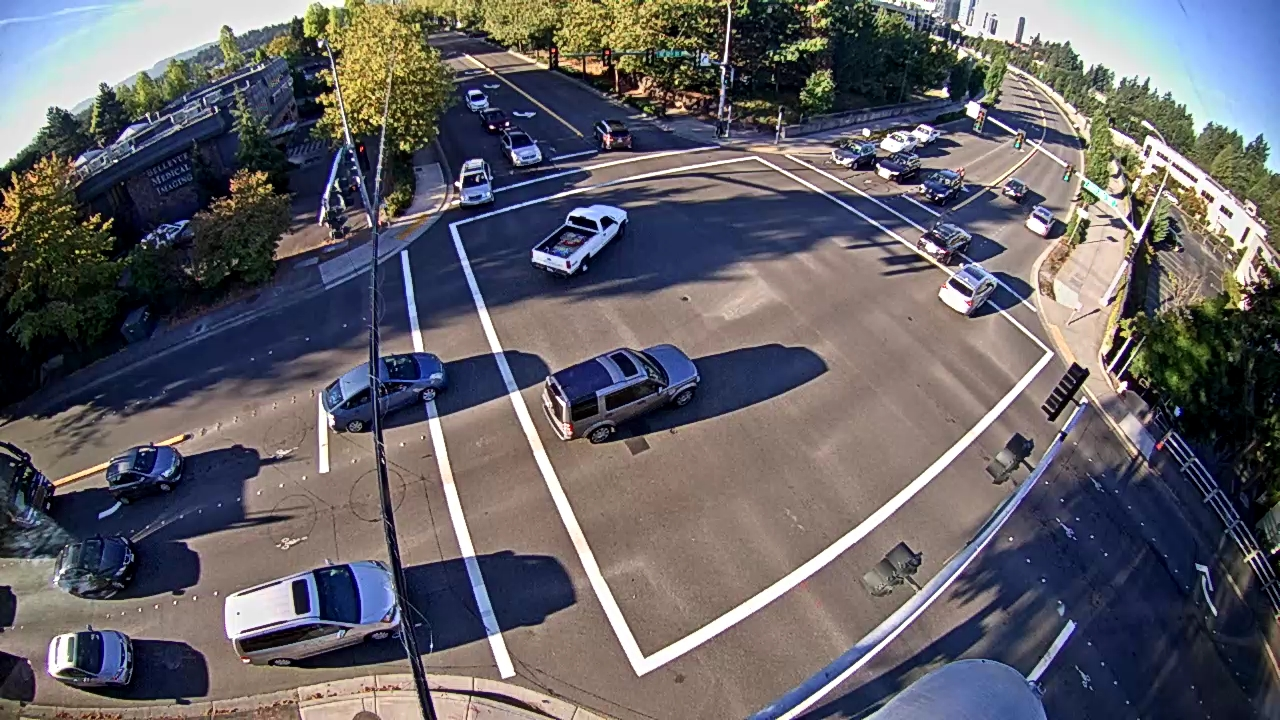
\includegraphics[width=1\columnwidth]{dataset_samples/Bellevue_116th_NE12th.JPG}
    \caption{Bellevue NE kereszteződés}
    \label{fig: BellevueNE}
\end{figure}
\begin{figure}
    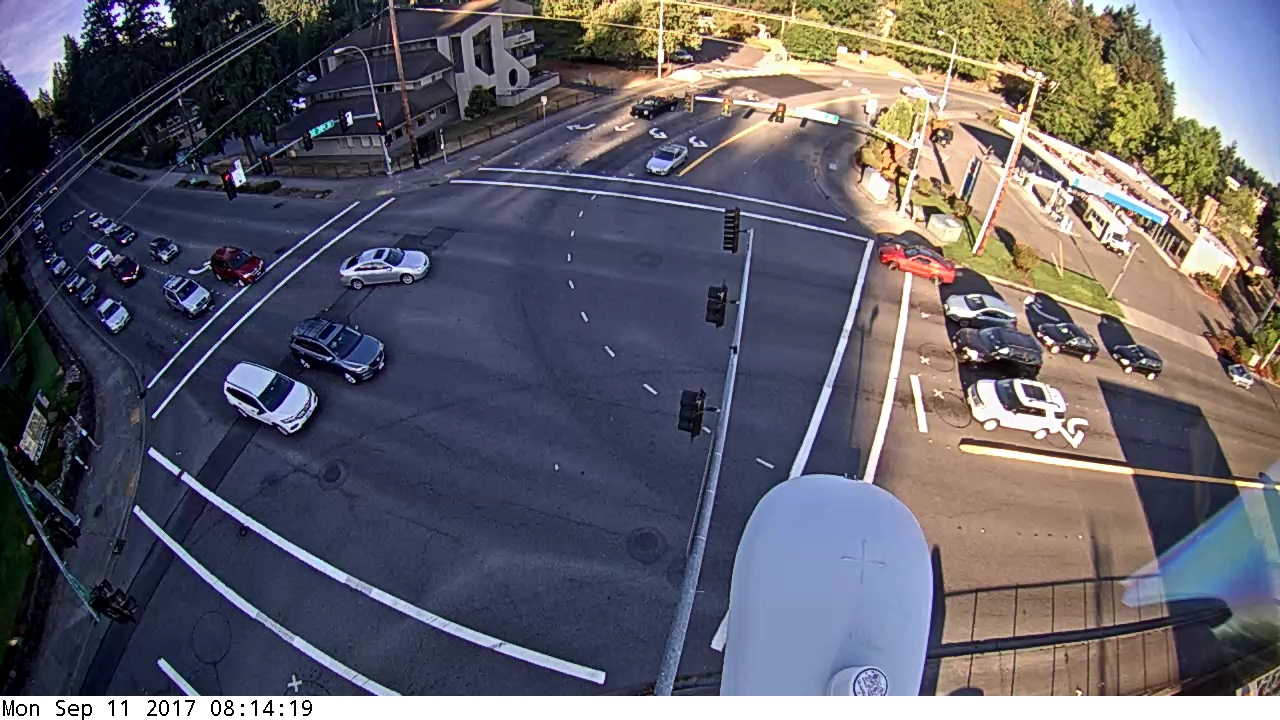
\includegraphics[width=1\columnwidth]{dataset_samples/Bellevue_150th_SE38th.JPG}
    \caption{Bellevue SE kereszteződés}
    \label{fig: BellevueSE}
\end{figure}
\begin{figure}
    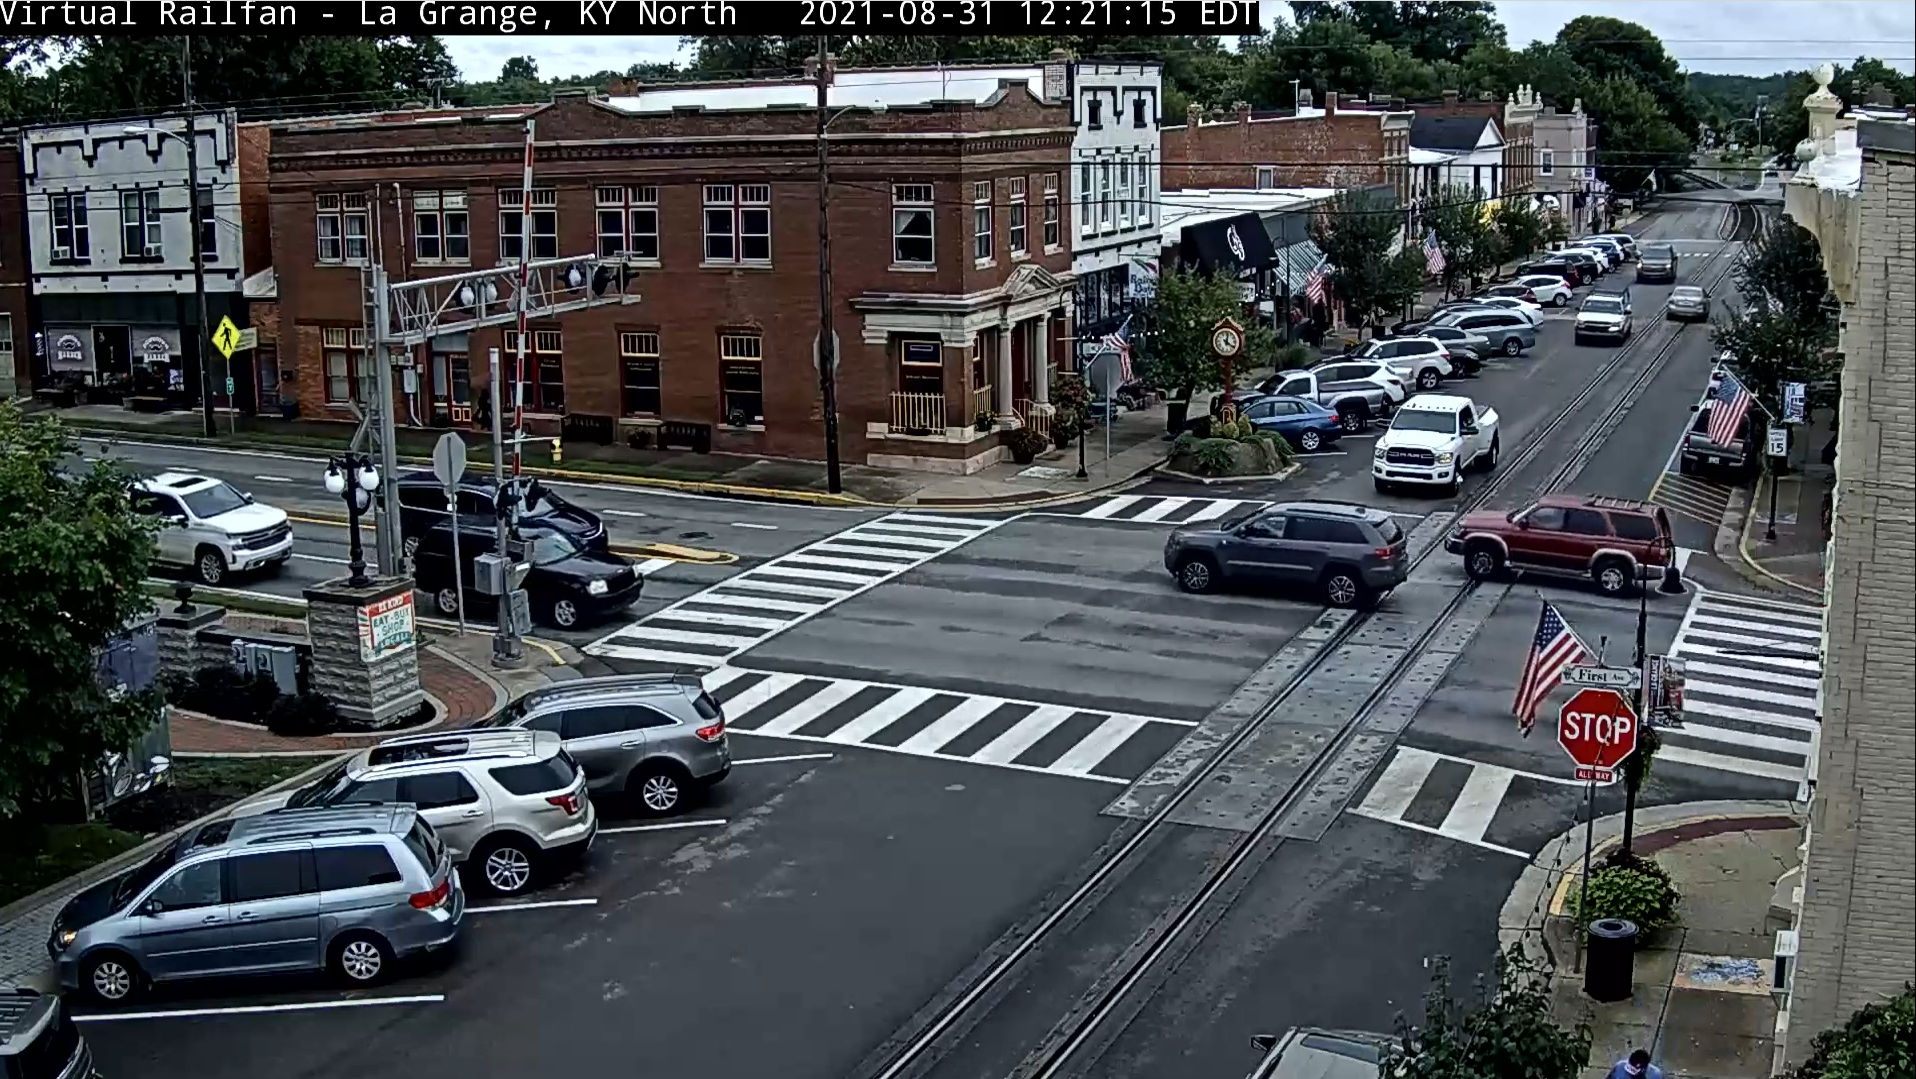
\includegraphics[width=1\columnwidth]{dataset_samples/lagrange_kynorth.png}
    \caption{La Grange KY North}
    \label{lagrangekynorth}
\end{figure}

\newpage
\section{Felhaszált módszerek}
\subsection{Kapcsolódó kutatások} 
Sok ITS-el kapcsolatos kutatásban tárgyalják a forgalom folyás (traffic flow) előrejelzését. \cite{PAUL2017177} összehasonlítja az eddig
kutatott és használt modellek, mint például Kálmán-szűrő, k-nearest neighbor (k-NN), mesterséges neurális hálók, stb., pontosságát és
sebességét, ezen modellek továbbkutatását, mivel egyre növekednek a különböző szenzorok által  begyűjtött traffic flow adatok, így ez a terület belépett
a \emph{Big Data} korszakába. \cite{10.1371/journal.pone.0253868} is a traffic flow előrejelzését és generálását tárgyalja, Floating Car Data (FCD)
adathalmazokon betanított, Hosszú-Rövid-Távú memóriájú és Generatív versengő hálókkal.
\subsection{YOLO}
YOLO (You Only Look Once) egy nagyon hatékony objektumdetektáló algoritmus, amely képes nagyon gyorsan észlelni és besorolni az objektumokat egy képen vagy videón.
A YOLO algoritmus működése a következő lépésekből áll:
\begin{enumerate}
    \item Bemeneti kép előkészítése: A kép előkészítése magában foglalja a normalizálást és a méretarányhoz való igazítást annak érdekében, hogy az YOLO algoritmus hatékonyan dolgozhasson a képpel.
    \item Vektor előállítása: A YOLO algoritmus a bemeneti képet a vektorizálás segítségével elemzi, amelynek eredménye egy tensor lesz, amely az objektumok lokalizációjához és azok osztályozásához szükséges információkat tartalmazza.
    \item Konvolúciós hálózat alkalmazása: A YOLO algoritmus egy kiterjedt konvolúciós hálózatot alkalmaz a vektorra, amelynek célja az objektumok lokalizálása és azok osztályozása.
    \item Objektum lokalizálása és osztályozása: A YOLO algoritmus az általa előállított tenzoron keresztül végzi az objektumok lokalizálását és azok osztályozását. Az algoritmus meghatározza az objektumok koordinátáit és a hozzájuk tartozó osztályt.
\end{enumerate}
A YOLO algoritmus előnye, hogy nagyon gyors és hatékonyan kezeli az objektumok lokalizálását és azok osztályozását. Az algoritmus gyakran jobb teljesítményt nyújt, mint a hasonló módszerek, és a különböző objektumokat a bemeneti képen gyorsan és hatékonyan azonosítja. Azonban az YOLO algoritmus hibázhat, ha az objektumok nagyon hasonlóak egymáshoz vagy a háttérhez, és nagyobb hibát eredményezhet, ha az objektumok nagyon kicsik a képen.
Legfrissebb változata a Yolov7 felülmúlja sebességben és pontosságban a modern konvolúciós hálókat (lásd \ref{fig:Yolov4chart}). Beágyazott rendszerekben és videókártyákon is egyaránt jó a teljesítménye, ezért az ITS területén alkalmazható.
% \begin{figure}[htbp]
%     \begin{description}
%         \centering
%         \item[YOLOv3 perfomance over other CNN models.]
%     \end{description}
%     \centering
%     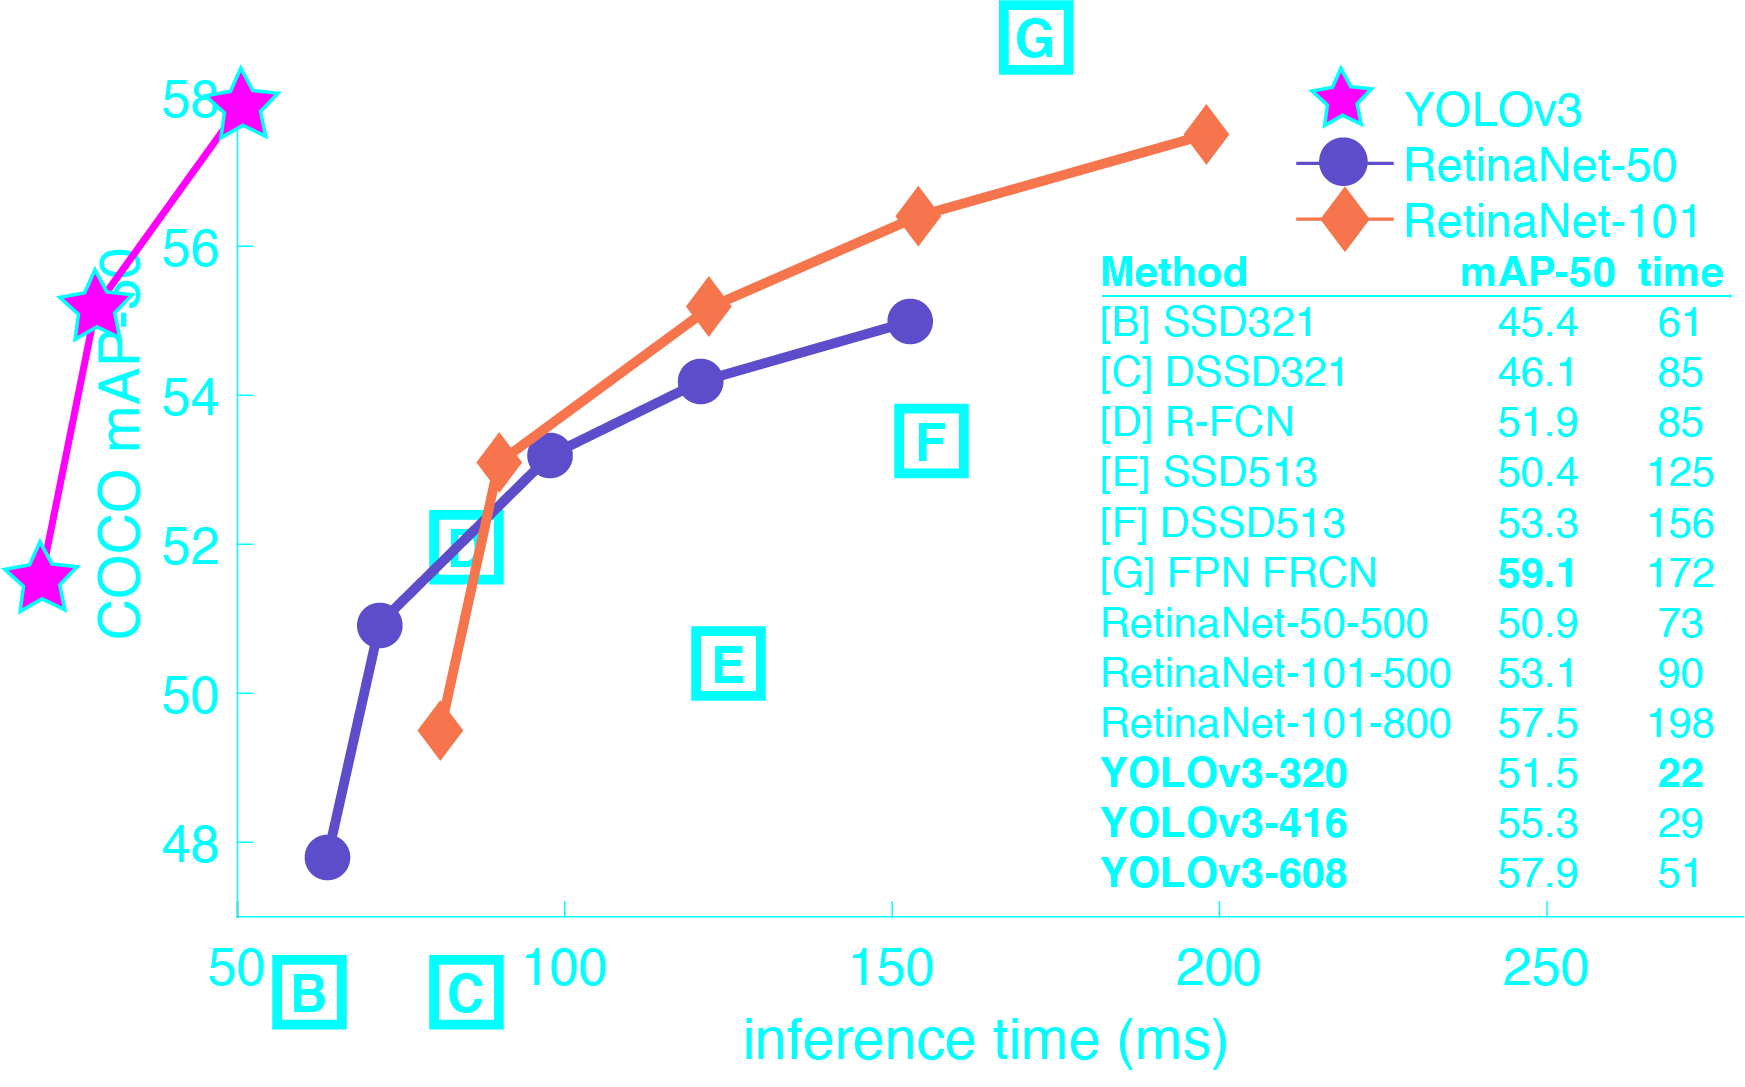
\includegraphics[width=0.6\columnwidth]{yolov3_perf.png}
%     \caption{YOLOv3 Performance}
%     \label{fig:Yolov3chart}
% \end{figure}
\begin{figure}[htbp]
    \begin{description}
        \centering
        \item[YOLOv4 perfomance over other CNN models.]
    \end{description}
    \centering
    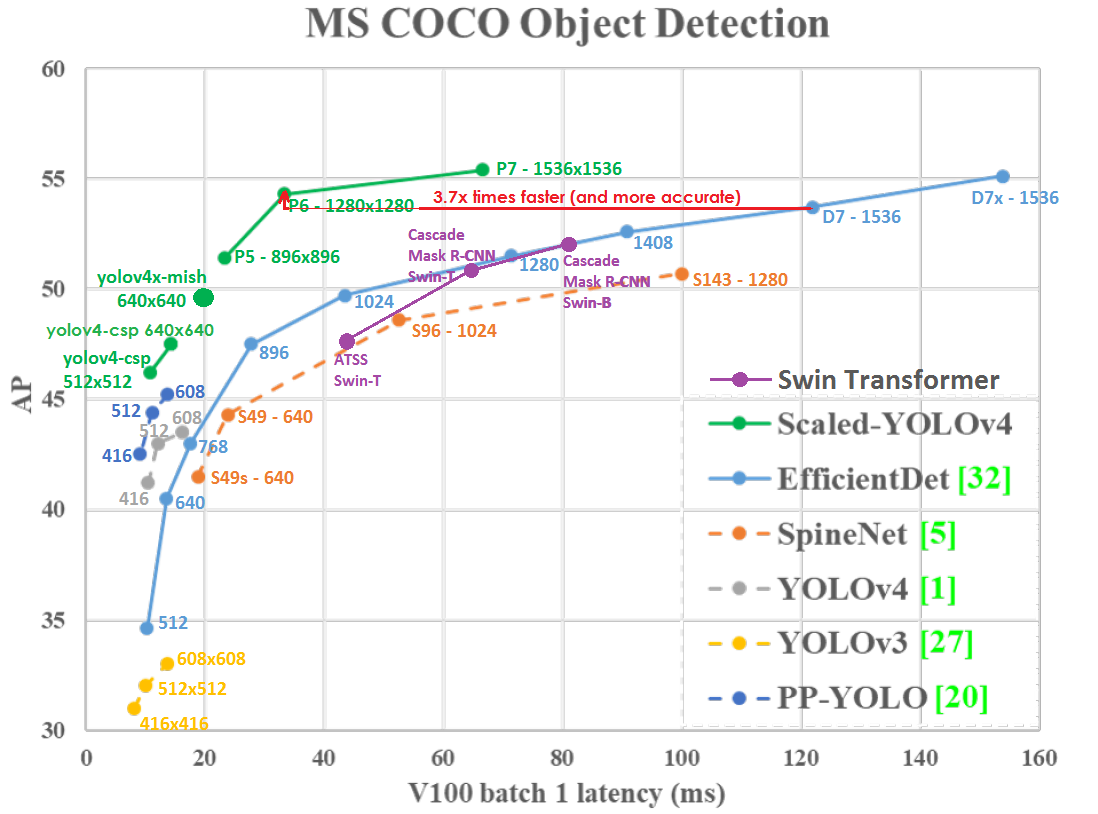
\includegraphics[width=0.75\columnwidth]{yolov4_perf.png}
    \caption{YOLOv4 Performance}
    \label{fig:Yolov4chart}
\end{figure}
\begin{figure}[htbp]
    \begin{description}
        \centering
        \item[YOLOv7 perfomance over other yolo models.]
    \end{description}
    \centering
    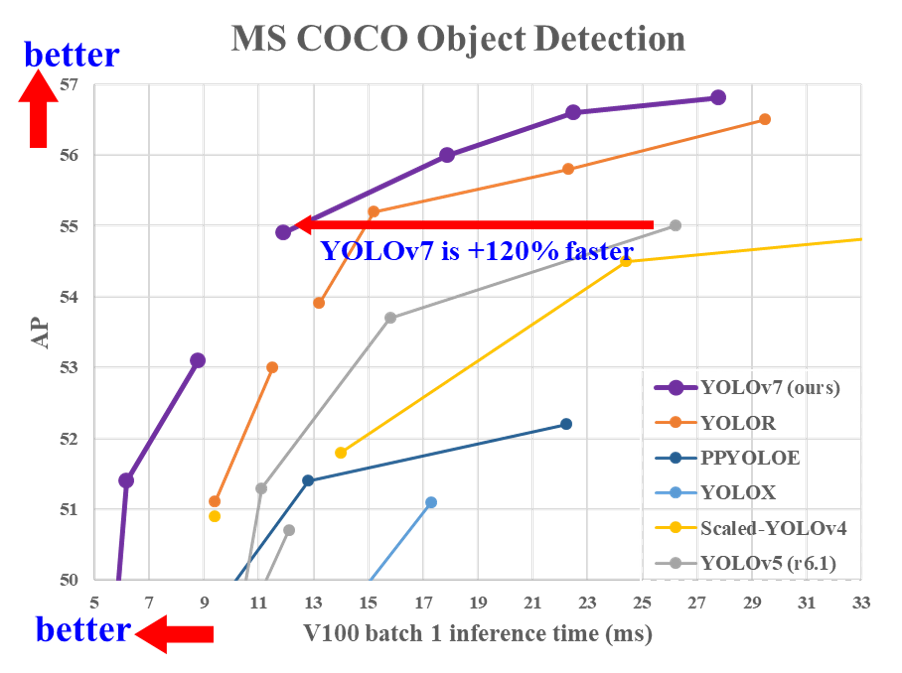
\includegraphics[width=0.75\columnwidth]{performance.png}
    \caption{YOLOv7 Performance}
    \label{fig:Yolov7chart}
\end{figure}
\subsection{DeepSORT}
\paragraph{DeepSORT (Deep Learning to Track Multi-Object in Video Sequences)} egy objektumkövetési algoritmus, amely a Deep Learning és a SORT (Simple Online and Realtime Tracking) algoritmusokat kombinálja. A DeepSORT algoritmus célja, hogy pontosan kövesse az objektumokat a videófelvételen, és azonosítsa azokat egyedi azonosítókkal.
Ez egy kiterjesztése a SORT (Simple Online and Realtime Tracking) algoritmusnak, amely az egymást követő képkockákban található detekciókhoz való társításon alapul a magyar algoritmus segítségével.
\paragraph{A DeepSORT algoritmus működése a következő lépésekből áll:}
\begin{enumerate}
    \item Objektumdetektálás: Az algoritmus először objektumdetektálással azonosítja az összes objektumot a videófelvételen, például a YOLO objektumdetektáló algoritmust használva.
    \item Jellemzők kinyerése: A DeepSORT az objektumok jellemzőit (pl. méret, sebesség, szín) kinyeri, hogy a következő lépésben a következő objektumot azonosítani tudja.
    \item Objektumazonosítás: Az algoritmus használ egy ``tracklet" nevű algoritmust, hogy azonosítsa és kövesse az objektumokat az időben. A ``tracklet" az objektum jellemzőit használja, hogy azonosítsa az adott objektumot a videófelvétel további részein.
    \item Címkézés: Az objektumokat azonosítják egyedi azonosítókkal, hogy az algoritmus megkülönböztethesse azokat az egyes videófelvételeken.
    \item Korszakosítás: A DeepSORT algoritmus általánosan a Kálmán-szűrőt használja, amely folyamatosan frissíti az objektumok helyzetének becslését. A Kálmán-szűrő segít az algoritmusnak megjósolni az objektumok további helyzetét a videófelvétel során.
\end{enumerate}
A DeepSORT algoritmus előnye, hogy nagyon stabil és pontos objektumkövetést biztosít akkor is, ha az objektumok átmennek más objektumok mögött vagy ha azok mozgása elég bonyolult. Az algoritmus nagyobb pontosságot nyújt a hagyományos objektumkövetési algoritmusokhoz képest, és képes megbirkózni a nagy sebességű objektumok követésével is. Azonban az algoritmus nagyobb számítási erőforrásokat igényel, és magasabb szintű számítási készséget igényel az implementáláshoz.
\begin{figure}
    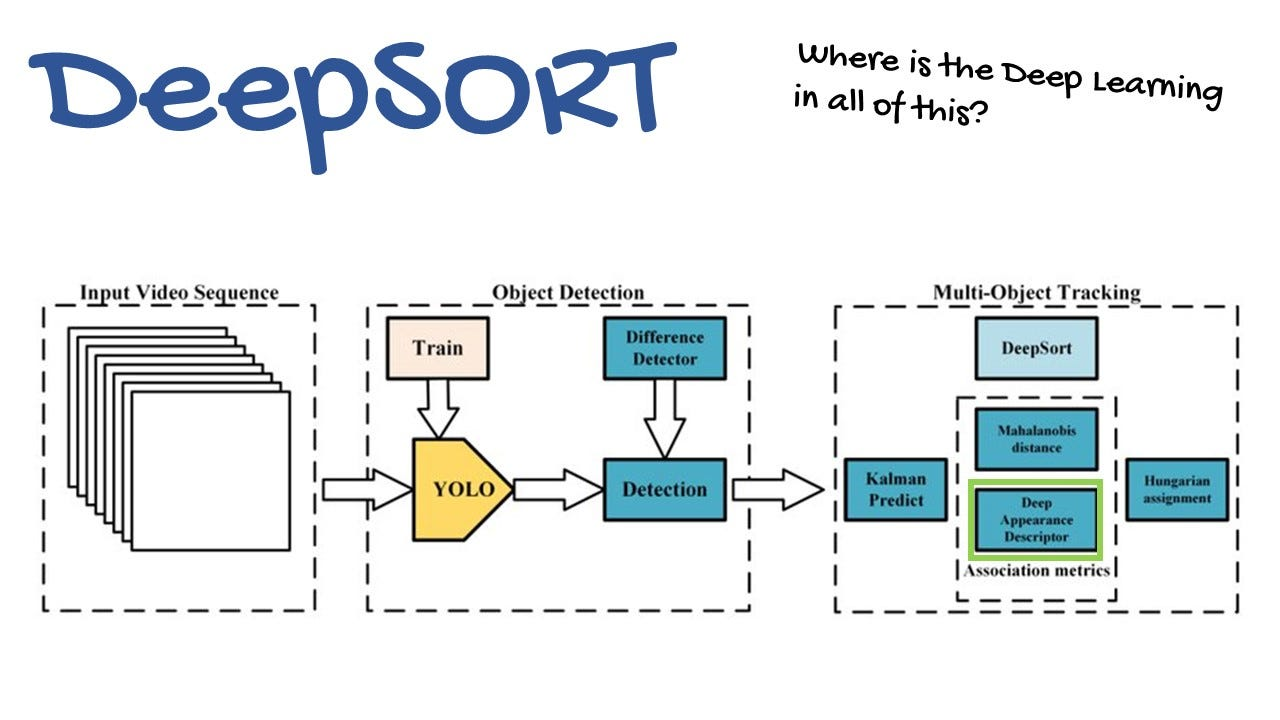
\includegraphics[width=1\columnwidth]{deepsort_yolo_figs/deepsort_block_diagram.jpg}
    \caption{Objektum követés}
    \label{ObjectTracking}
\end{figure}

\newpage
\section{Adathalmaz kialakítása és feldolgozása}
A kutatás során saját adathalmazok kialakítására volt szükség. Az adatok begyűjtésére és eltárolására saját alkalmazást és keretrendszert
fejlesztettünk ki. A szoftver keretrendszert python nyelven írtuk meg, a forráskód ezen a linken megtatlálható \url{http://github.com/Pecneb/computer_vision_research}.
A fejlesztés során a következő programkönyvtárakat használtuk OpenCV \cite{opencv_library}, Numpy \cite{harris2020array}, Pandas \cite{reback2020pandas},
Scikit-Learn \cite{scikit-learn}, Matplotlib \cite{Hunter:2007}, SQLite \cite{sqlite2020hipp}, Joblib \cite{joblib_library}. Az adathalmazokat SQLite adatbázisban és
joblib fájlokban tároltuk el.
\paragraph{OpenCV} A videók feldolgozásához és a képkockák feldolgozásához használtuk az OpenCV könyvtárat. Az OpenCV egy nyílt forráskódú programkönyvtár, amelyet a gépi látás és a gépi tanulás alkalmazásokhoz fejlesztettek ki. Az OpenCV-t C++ nyelven írták, de támogatja a Python, Java és MATLAB programozási nyelveket is. Az OpenCV-t a BSD licenc alatt terjesztik, és szabadon használható és módosítható.
\paragraph{Numpy} A Numpy egy Python könyvtár, amelyet a tudományos számításokhoz fejlesztettek ki. A Numpy-t C és Fortran nyelveken írták. A Numpy-t a tudományos számításokhoz, például a mátrixműveletekhez, a mátrixok létrehozásához és a lineáris algebrai műveletekhez használják.
\paragraph{Pandas} A Pandas egy Python könyvtár, amelyet a nagy teljesítményű adatelemzéshez és adatmanipulációhoz fejlesztettek ki. Numpy könyvtárra épül.
\paragraph{Scikit-Learn} A Scikit-Learn egy Python könyvtár, amelyet a gépi tanuláshoz fejlesztettek ki. A Scikit-Learn a Numpy és a SciPy könyvtárakra épül.
\paragraph{Matplotlib} A Matplotlib egy Python könyvtár, amelyet a képek és grafikonok megjelenítéséhez fejlesztettek ki. A Matplotlib-et a Numpy könyvtárra építették.
\paragraph{SQLite} Az SQLite egy nyílt forráskódú relációs adatbázis-kezelő rendszer, amelyet a beágyazott adatbázisokhoz fejlesztettek ki. Az SQLite-t C nyelven írták.
\paragraph{Joblib} A Joblib egy Python könyvtár, amelyet a Python objektumok hatékony szerializálásához és deszerializálásához, számításigényes feladatok paralellizálására fejlesztettek ki. A Joblib-et a Numpy könyvtárra építették.

\newpage
\subsection{Adatstruktúra}
Az adatstruktúrát SQL schema-ként, és python osztály-ként is definiáltuk.
\paragraph{SQL schema} Az SQL schema a következőképpen néz ki:
\begin{minted}{sql}
CREATE TABLE IF NOT EXISTS objects (
            objID INTEGER PRIMARY KEY NOT NULL,
            label TEXT NOT NULL
        );
CREATE TABLE IF NOT EXISTS detections (
            objID INTEGER NOT NULL,
            frameNum INTEGER NOT NULL,
            confidence REAL NOT NULL,
            x REAL NOT NULL,
            y REAL NOT NULL,
            width REAL NOT NULL,
            height REAL NOT NULL,
            vx REAL NOT NULL,
            vy REAL NOT NULL,
            ax REAL NOT NULL,
            ay REAL NOT NULL,
            vx_c REAL NOT NULL,
            vy_c REAL NOT NULL,
            ax_c REAL NOT NULL,
            ay_c REAL NOT NULL,
            FOREIGN KEY(objID) REFERENCES objects(objID)
        );
CREATE TABLE IF NOT EXISTS metadata (
            historyDepth INTEGER NOT NULL,
            yoloVersion TEXT NOT NULL,   
            device TEXT NOT NULL,
            imgsize INTEGER NOT NULL,
            stride INTEGER NOT NULL,
            confidence_threshold REAL NOT NULL,
            iou_threshold REAL NOT NULL,
            k_velocity REAL NOT NULL,
            k_acceleration REAL NOT NULL
        );
\end{minted}
Minden követett objektum egyedi azonosítóval lett ellátva. Az objektumhoz tartozó detektálások külön táblába lettek kiszervezve,
ahol az \textit{objID} idegen kulccsal kapcsoljuk az \textit{objektumok} táblához. Egy objektumhoz az egyedi azonosítón kívül
tartozik egy \textit{label}, amit a YOLO objektum detektálótól kap, ez lehet pl. autó, személy, teherautó, stb. Az objektumokhoz
tartózó detektálások tartalmazzák a képkocka számát, amikor a detektálás történt, a konfidenciát, hogy mennyire biztos az
objektumfelismerő a hozzárendelt \textit{label}-ben, az objektum \begin{math}x,y\end{math} koordinátáját, az objektum szélességét
\begin{math}width\end{math} és magasságát \begin{math}width\end{math}, sebességét \begin{math}v_x,v_y\end{math} és gyorsulását \begin{math}a_x,a_y\end{math},
amik a deepSORT által kalkulált értékek, így még külön a koordinátákból kiszámolt \begin{math}v_{x_c},v_{y_c}\end{math} sebességet és
\begin{math}a_{x_c},a_{y_c}\end{math} gyorsulást is eltároltuk.
Ezek mellett még a konfigurációs adatokat is külön táblában tároljuk, hogy később meg lehessen ismételni a detektálást.
A koordinátákat a videó méretének megfelelően leskálázzuk 0 - 1 értékek köré. Ha a videókép szélesség \begin{math}w\end{math}, magasság \begin{math}h\end{math},
akkor a képarány \begin{math}r = \frac{w}{h}\end{math}, és az eltárolt koordináták
\newpage
\begin{equation}x = \frac{x_0}{w} \cdot r, y = \frac{y_0}{w} \cdot r\end{equation}
\begin{equation}v_x = \frac{v_{x_0}}{w} \cdot r, v_y = \frac{v_{y_0}}{w} \cdot r\end{equation}
\begin{equation}a_x = \frac{a_{x_0}}{w} \cdot r, a_y = \frac{a_{y_0}}{w} \cdot r\end{equation}
\begin{equation}v_{x_c} = \frac{v_{xc0}}{w} \cdot r, v_{y_c} = \frac{v_{yc0}}{w} \cdot r\end{equation}
\begin{equation}a_{x_c} = \frac{a_{xc0}}{w} \cdot r, a_{y_c} = \frac{a_{yc0}}{w} \cdot r\end{equation}.

\paragraph{Python osztályok} A python osztályokhoz a python beépített Dataclass könyvtárat használtam, ami sok boilerplate kódot spórol meg.
Detektálások és Trajektóriák reprezentálására, összehasonlítására és numpy-vel való műveletekre nagyon hasznos.
\paragraph{Python Detection osztály}
\begin{minted}{python}
    @dataclass
    class Detection:
        label: str
        confidence: float
        X: float
        Y: float
        Width: float
        Height: float
        frameID: int
        VX: float = field(init=False)
        VY: float = field(init=False)
        AX: float = field(init=False)
        AY: float = field(init=False)
        objID: int = field(init=False)

        def __repr__(self) -> str:
            return f"Label: {self.label}, \
                Confidence: {self.confidence}, \
                X: {self.X}, Y: {self.Y}, Width: \
                {self.Width}, Height: {self.Height}, Framenumber: {self.frameID}"

        def __eq__(self, other) -> bool:
            if self.label != other.label:
                return False
            if self.confidence != other.confidence:
                return False
            if self.X != other.X:
                return False
            if self.Y != other.Y:
                return False
            if self.Width != other.Width:
                return False
            if self.Height != other.Height:
                return False
            if self.frameID != other.frameID:
                return False
            return True
\end{minted}

\paragraph{Python TrackedObject osztály} tárolja el egy objektum összes detektálását, és a detektálásokból kiszámolt sebességeket és gyorsulásokat.
A trajektória osztály számon tartja az objektum állapotát, hogy mennyi ideje történt az utolsó detektálás és hogy mozog e vagy sem.
\begin{minted}{python}
    @dataclass
    class TrackedObject:
        objID: int
        label: int = field(init=False)
        futureX: list = field(init=False)
        futureY: list = field(init=False)
        history: List[Detection] = field(init=False)
        history_X: np.ndarray = field(init=False)
        history_Y: np.ndarray = field(init=False)
        history_VX_calculated: np.ndarray = field(init=False)
        history_VY_calculated: np.ndarray = field(init=False)
        history_AX_calculated: np.ndarray = field(init=False)
        history_AY_calculated: np.ndarray = field(init=False)
        isMoving: bool = field(init=False)
        time_since_update: int = field(init=False)
        max_age: int
        mean: list = field(init=False)
        X: int
        Y: int
        VX: float = field(init=False)
        VY: float = field(init=False)
        AX: float = field(init=False)
        AY: float = field(init=False)
        _dataset: str = field(init=False)

        def __init__(self, id: int, first: Detection, max_age: int = 30):
            self.objID = id
            self.history = [first]
            self.history_X = np.array([first.X])
            self.history_Y = np.array([first.Y])
            self.history_VX_calculated = np.array([])
            self.history_VY_calculated = np.array([])
            self.history_VT = np.array([])
            self.history_AX_calculated = np.array([])
            self.history_AY_calculated = np.array([])
            self.X = first.X
            self.Y = first.Y
            self.VX = 0
            self.VY = 0
            self.AX = 0
            self.AY = 0
            self.history[-1].VX = self.VX
            self.history[-1].VY = self.VY
            self.history[-1].AX = self.AX
            self.history[-1].AY = self.AY
            self.label = first.label
            self.isMoving = False
            self.max_age = max_age
            self.time_since_update = 0
            self.mean = []
            self._dataset = ""
\end{minted}

\subsection{Objektumdetektálás}
Az objektumdetektáláshoz a fent említett YOLO modellt haszáltuk. Kutatásunk kezdetekor, a YOLO 4-es verziójával kezdtünk dolgozni,
de később átváltottunk a jobb pontosságot és sebességet ígérő 7-es verzióra.
% \subsubsection{YOLOv4}
% YOLO 4-es verzióját, C-ben implementálták. Hogy fel tudjuk használni, írnunk kellett egy python API-t, amit meg tudtunk hívni a
% detektáló programunkban.
\subsubsection{YOLOv7}
A Yolov7 pythonban azon belül is pytorch-ban van implementálv. Hogy használni tudjam saját API-t kellett fejlesztenem hozzá.
Az API része a képek előfeldolgozása, beadása a neurális hálózatba majd utófeldolgozása, hogy emberileg értelmezhető detektálásokat
kapjunk. (lásd \ref{fig:Yolov7chart}).
Yolov7 felhasználásához objektum orientált megközelítést használtam. Egy Yolov7 osztályt hoztam létre, hogy elvégezze a detektálási feleadaokat,
és könnyen olvasható és használható legyen.
\subsection{Objektumkövetés}
Ahhoz, hogy trajektóriák alapján tudjunk szabályosságokat felismerni a forgalomban, pontos objektumkövetésre volt szükségünk. Eleinte
saját objektumkövető algoritmust használtunk, ami deketálások euklideszi távolsága alapján próbálta meg követni az objektumokat.
Ezzel az volt a gond, hogy hosszabb kitakarás után nem találta meg az objektumot, így egy új objektumnak számított, ami a kép
közepéből bukkant fel. Ennek a problémának a kiküszöbölésére próbáltuk ki a DeepSORT algoritmust.
\subsubsection{DeepSORT}
A DeepSORT algoritmus pythonban implementált változatát integráltuk a mi programunkba. Yolo-hoz hasonlóan egy oszályként implementáltam az objektumkövetési
interface-t.

\newpage
\subsection{Objektum Orientált Implementáció}
Az objektum detektálási és követése pipeline-t egy objektum orientált megközelítéssel valósítottam meg. A programban 4 fő osztályt hoztam létre. A osztály architektúra diagramja \ref{fig:ClassDiagram} ábrán látható.
A részletes implementációs dokumentáció a mellékletben található. A forráskód pedig a korábban említett github oldalon található \url{http://github.com/Pecneb/computer_vision_research}.
\paragraph{Yolov7} osztály felelős a képek előfeldolgozásáért, az objektumok detektálásálért, majd utófeldolgozásáért.
Az előfeldolgozáshoz írt saját kódban (\textit{preprocess()}) az opencv-vel bekért képeket a Yolov7 által elvárt formátumra alakítom.
A Yolov7 640x640-es képeket vár, ezért a képeket erre a méretre skálázom.
\begin{minted}{python3}
def preprocess(self, img0: np.ndarray) -> np.ndarray:
    # Padded resize
    if len(img0.shape) == 3:  # check for single image
        self._logger.debug(f"Input image shape: {img0.shape}")
        img = letterbox(img0, new_shape=self.imgsz, stride=self.stride)[0]
        img = np.expand_dims(img, axis=0)
    else:  # check for multiple images as input
        img = [letterbox(x, new_shape=self.imgsz, stride=self.stride)[
            0] for x in img0]
    img = np.stack(img, 0)
    # Convert
    # BGR to RGB, to 3x640x640
    img = img[:, :, :, ::-1].transpose(0, 3, 1, 2)
    # store img in memory in on place, not in segments for faster lookup
    img = np.ascontiguousarray(img)
    return img
\end{minted}

Az utófeldolgozásnál (\textit{postprocess()}) a meghatározott konfidencia érték és IoU (Intersection over Union) érték alapján szűröm a detektálásokat.
A neurális háló a képen detektált objektumok keretét, az objektumok osztályát és a detektálás konfidencia értékét adja vissza.
Az objektum kereteket a kép méretére skálázom, hogy később ki tudjam rajzolni a képre.
\begin{minted}{python3}
def postprocess(
    self, 
    pred: torch.Tensor, 
    im0: np.ndarray, 
    im: np.ndarray, 
    show: bool = True) -> List:
    _pred = non_max_suppression(
        pred, conf_thres=self.conf_thres, iou_thres=self.iou_thres)
    detections_adjusted = []
    for det in _pred:
        if len(det):
            det[:, :4] = scale_coords(
                im.shape[1:], det[:, :4], im0.shape).round()
            for *xyxy, conf, cls in det:
                if show:
                    plot_one_box(xyxy, im0, label=self.names[int(
                        cls)], color=self.colors[int(cls)], line_thickness=3)
                # convert to center coords, width, height format
                bbox = xyxy2xywh(torch.tensor(xyxy).view(1, 4))
                label = self.names[int(cls)]
                detections_adjusted.append(
                    [label, conf.item(), bbox[0, :].numpy()])
    return detections_adjusted
\end{minted}
\paragraph{DeepSORT} osztály felelős a detektálások követéséért, és a trajektóriák kialakításáért.
\paragraph{TrajectoryNet} osztály kezeli az általunk tanított gépi tanulási modelleket, a feature vektorok előállítását és osztályozást.
\paragraph{Detector} osztály fogja össze az előbb felsorolt osztályokat. Inicializálja a bemeneti és kimeneti adatokat. Végig itertál a videó képkockáin és futtatja a detektáló és követő algoritmusokat.
\paragraph{Detector \textit{run()}} metódusban implementáltam az objektum detektálás, követés és trajektória predikciós pipeline-t (lásd \ref{fig:ComponentDiagram}). A kép egy képkocka feldolgozását mutatja be.

\begin{figure}[H]
    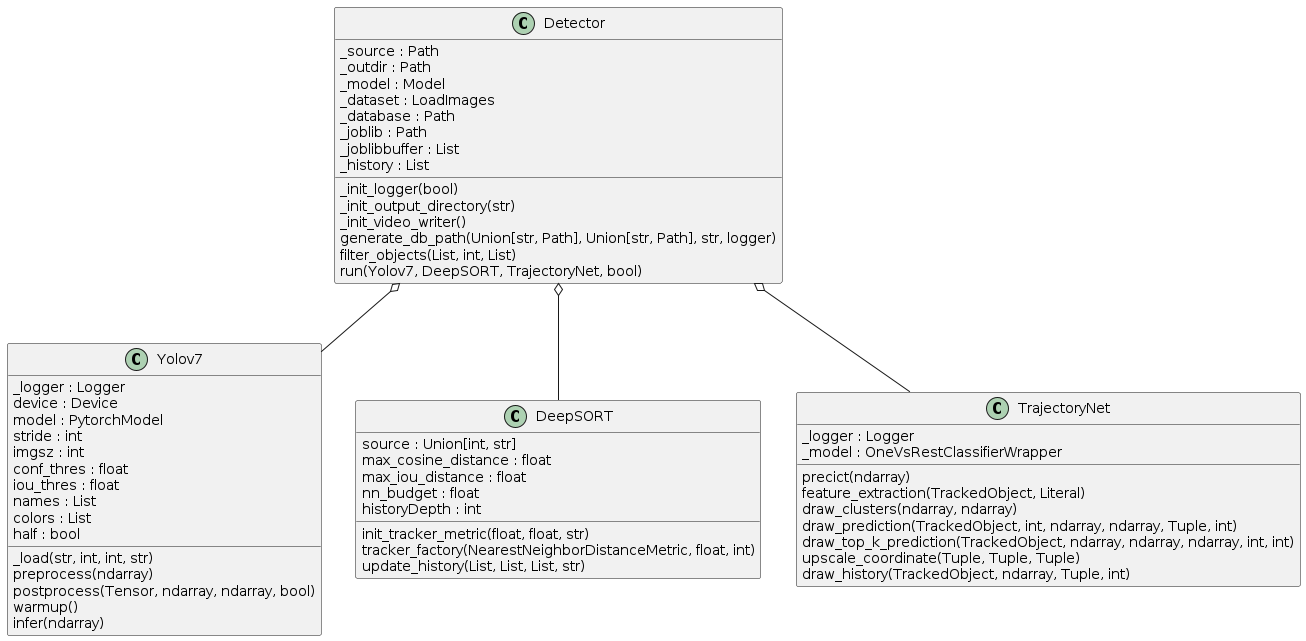
\includegraphics[width=1\columnwidth]{ClassArchitectureDiagram.png}
    \caption{Osztály diagram}
    \label{fig:ClassDiagram}
\end{figure}


\begin{figure}[H]
    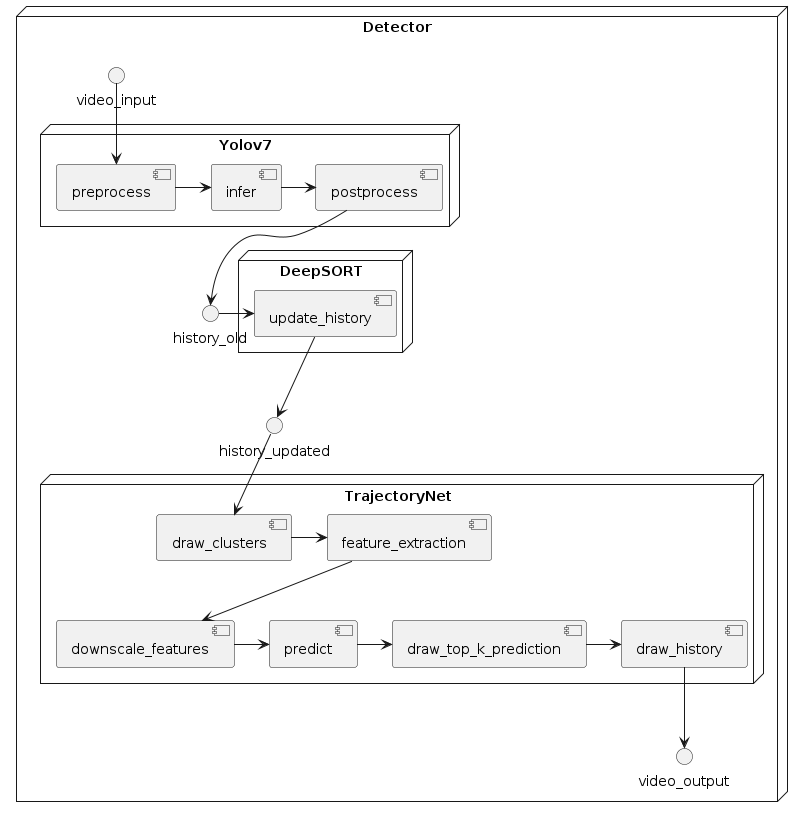
\includegraphics[width=1\columnwidth]{ComponentDiagramDetection.png}
    \caption{Komponens diagram}
    \label{fig:ComponentDiagram}
\end{figure}


\newpage
\subsection{Implementáció dokumentálása}
A programok dokumentálására a Sphinx \cite{brandl2021sphinx} keretrendszert használtuk. A Sphinx egy dokumentációs generátor, amely a megfelelően dokumentált
Python kódból (ezalatt a Python nyelvhez tartozó dokumentációs sztringeket értjük) HTML és Latex dokumentációt készít. Egy ilyen dokumentációs sztringre példa.
A generált dokumentáció a mellékletben található.
\begin{minted}{python}
   def make_4D_feature_vectors(trackedObjects: List) -> np.ndarray:
    """
    Create 4D feature vectors from tracks.

    Parameters
    ----------
    trackedObjects : list
        List of tracked objects.

    Returns
    -------
    np.ndarray
        Numpy array of feature vectors.

    Notes
    -----
    The enter and exit coordinates are put in one vector, creating 4D vectors.
    v = [enterX, enterY, exitX, exitY]
    """
    featureVectors = np.array([np.array(
        [obj.history[0].X, obj.history[0].Y, obj.history[-1].X, obj.history[-1].Y])
        for obj in tqdm.tqdm(trackedObjects, desc="Feature vectors.")])
    return featureVectors 
\end{minted}


\newpage
\section{Klaszterezés}
A klaszterezés segítségével lehet az adathalmazból alőállítani az osztályozás alapjául szolgáló csoportokat. Ahhoz, hogy az
a rengeteg trajektóriából és detektálásból számunkra felhasználható információ keletkezzen, meg kell határoznunk feature
vectorokat, amik a trajektóriákra jellemző értékeket tartalmaznak. Ebben a feature térben fogja a klaszterező algoritmus
megtalálni az egymáshoz közeli, hasonló trajektóriákat.
\subsection{Adattisztítás}
A klaszterezés előtt a nyers adatokat fel kell dolgoznunk, hogy az esetleges hibás, zajos detektálások, trajektóriák miatt
kapjunk fals klasztereket. Az objektum detektálás és követés nem tökéletes, rossz fényviszonyok, hosszabb eltakarások miatt
a trajektóriák megszakadhatnak, ezért ki kell választani az egyben maradt trajektóriákat. Három általam implementált szűrő algoritmust használtam
az adathalmazon.
\paragraph{Trajektória hossz} Elsőnek a trajektóriák belépő és kilépő pontjainak az euklideszi távolsága alapján szűrtünk. Ezzel a szűréssel a zajos, félbeszakadt trajektóriákat szűrjük ki.
\begin{minted}{python}
def euclidean_distance(q1: float, p1: float, q2: float, p2: float):
    return (((q1-p1)**2)+((q2-p2)**2))**0.5

def filter_out_false_positive_detections_by_enter_exit_distance(
    trackedObjects, threshold):
    filteredTracks = list(filterfalse(lambda obj: euclidean_distance(
        obj.history[0].X, obj.history[-1].X, obj.history[0].Y, obj.history[-1].Y) 
            < threshold, trackedObjects))
    return filteredTracks
\end{minted}
Itt az euklideszi távolságot saját magam implementáltam, mert ez a megoldás bizonyult a leggyorsabbnak egyszerű, két 2 dimenziós pont között.
A numpy-nak több féle megoldását és a scipy könyvtárban található távolságszámítást is kipróbáltam, de ezek lassabbnak bizonyultak.
A méréshez a \textit{timeit} könyvtárat használtam. A mérés eredményeit a \ref{fig:EuclideanDistance} ábrán láthatjuk. A méréshez minden módszert $1000000$ alkalommal futtattam le, és az átlagot vettem.
Az $own$ címke jelenti a saját implementáció áltagos futás idejét.
A forrás kód a következő a numpy és scipy könyvtárakat használó függvényekhez:
\newpage
\begin{minted}{python}
def euclidean_distance(a, b):
    return (((a[0]-b[0])**2)+((a[1]-b[1])**2))**0.5

def euclidean_distance_np_linalg(a, b):
    return np.linalg.norm(a-b)

def euclidean_distance_np_sqrt(a, b):
    return np.sqrt(np.sum((a-b)**2))

def euclidean_distance_np_sqrt_square(a, b):
    return np.sqrt(np.sum(np.square(a-b)))

def euclidean_distance_np_dot(a, b):
    return np.sqrt((a-b).T @ (a-b))

def euclidean_distance_cdist(a, b):
    return cdist(a, b, metric='euclidean')    
\end{minted}

\begin{figure}[H]
    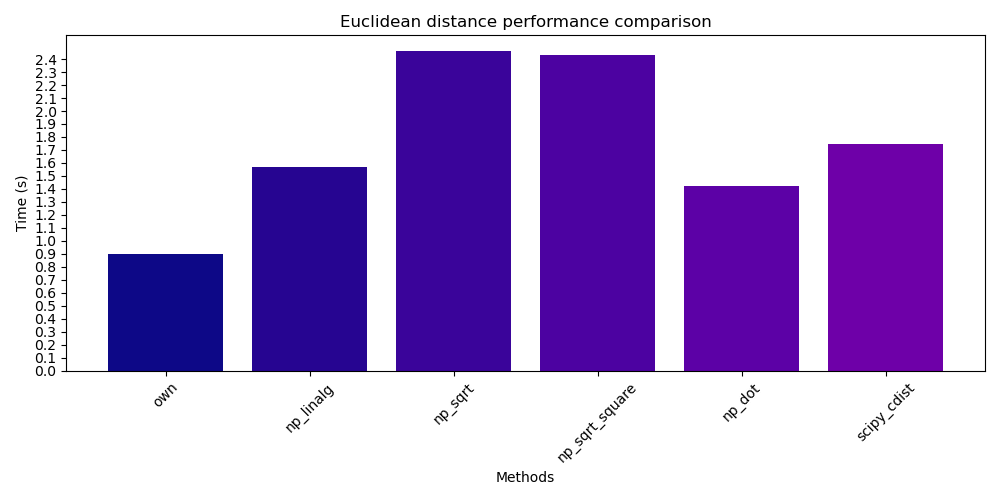
\includegraphics[width=1\columnwidth]{euclidean_distance_performance.png}
    \caption{Euklideszi távolság sebesség mérés}
    \label{fig:EuclideanDistance}
\end{figure}

\paragraph{Relatív szélekhez képesti távolság} Majd a kép széleit meghatározzuk min-max kiválasztással, és azokat a trajektóriákat választjuk ki, amiknek a szélektől meghatározott
távolságra vannak a belépő és kilépő pontjaik. Erre azért van szükség, mert ha belegondolunk, lehet hogy a kép egyik szélén valami eltakarja az utat pl. egy ház, és akkor az autók belépési pontjai a kép közepétől indulnak, ami nem jelenti azt, hogy az egy zajos, hibás trajektória, hanem ez a kereszteződés egy sajátossága.
\newpage
\begin{minted}{python}
def search_min_max_coordinates(trackedObjects):
    X = np.concatenate([o.history_X for o in trackedObjects], axis=None)
    Y = np.concatenate([o.history_Y for o in trackedObjects], axis=None)
    min_x = np.min(X)
    max_x = np.max(X)
    min_y = np.min(Y)
    max_y = np.max(Y)
    return min_x, min_y, max_x, max_y

def filter_out_edge_detections(trackedObjects, threshold):
    min_x, min_y, max_x, max_y = search_min_max_coordinates(trackedObjects)
    filteredTracks = []
    for obj in tqdm.tqdm(trackedObjects, desc="Filter out edge detections."):
        if (((obj.history[0].X <= min_x+threshold or 
            obj.history[0].X >= max_x-threshold) or
            (obj.history[0].Y <= min_y+threshold or 
            obj.history[0].Y >= max_y-threshold)) and
            ((obj.history[-1].X <= min_x+threshold or 
            obj.history[-1].X >= max_x-threshold) or
            (obj.history[-1].Y <= min_y+threshold or 
            obj.history[-1].Y >= max_y-threshold))):
            filteredTracks.append(obj)
    return filteredTracks
\end{minted}

\subsubsection{DeepSORT pontatlanság}
Kutatásunk során azt tapasztaltuk, hogy a DeepSORT és a YOLO pontatlanságai felerősítik egymást. A YOLO hajlamos néha táblákat
vagy rendőrlámpákat autóknak nézni, és ekkor a DeepSORT is elkezdi követni. Egy olyan hibáját is felfedeztük a DeepSORT-nak, hogy
egy objektumról áttapad a követés egy másik objektumra, ami fals trajektóriákat hoz létre. A DeepSORT-nak lehet finomhangolni a
paramétereit, ami nem bizonyult akkora javulásnak, ezért utólagos szűréssel kellett korrigálnunk ezt a hibát.
\paragraph{Áttapadásos zaj szűrése} Az algoritmus végig iterál a trajektóriák pontjain és kiszámítja az egymást követő detektálások euklideszi távoláságát, és ha egy küszöbérték felett vannak, akkor eldobjuk a trajektóriát.
Ez azért szükséges, mert a DeepSORT képes egymás közeli objektumokat összekeverni, és egyik objektumról a másikra áttapadni, ami hibás trajektóriákat eredményez.
A következő képeken láthatók a klaszterek szűrés előtt és után (lásd \ref{fig: Klaszterezés szűrő} \ref{fig: Klaszterezés szűrő2} \ref{fig: Klaszterezés szűrő3}), ahol a bal oldali oszlop reprezentálja a szűrés előtti klasztereket, a jobb oldali oszlop pedig a szűrés utáni klasztereket.

\begin{figure}[htbp]
    \centering
    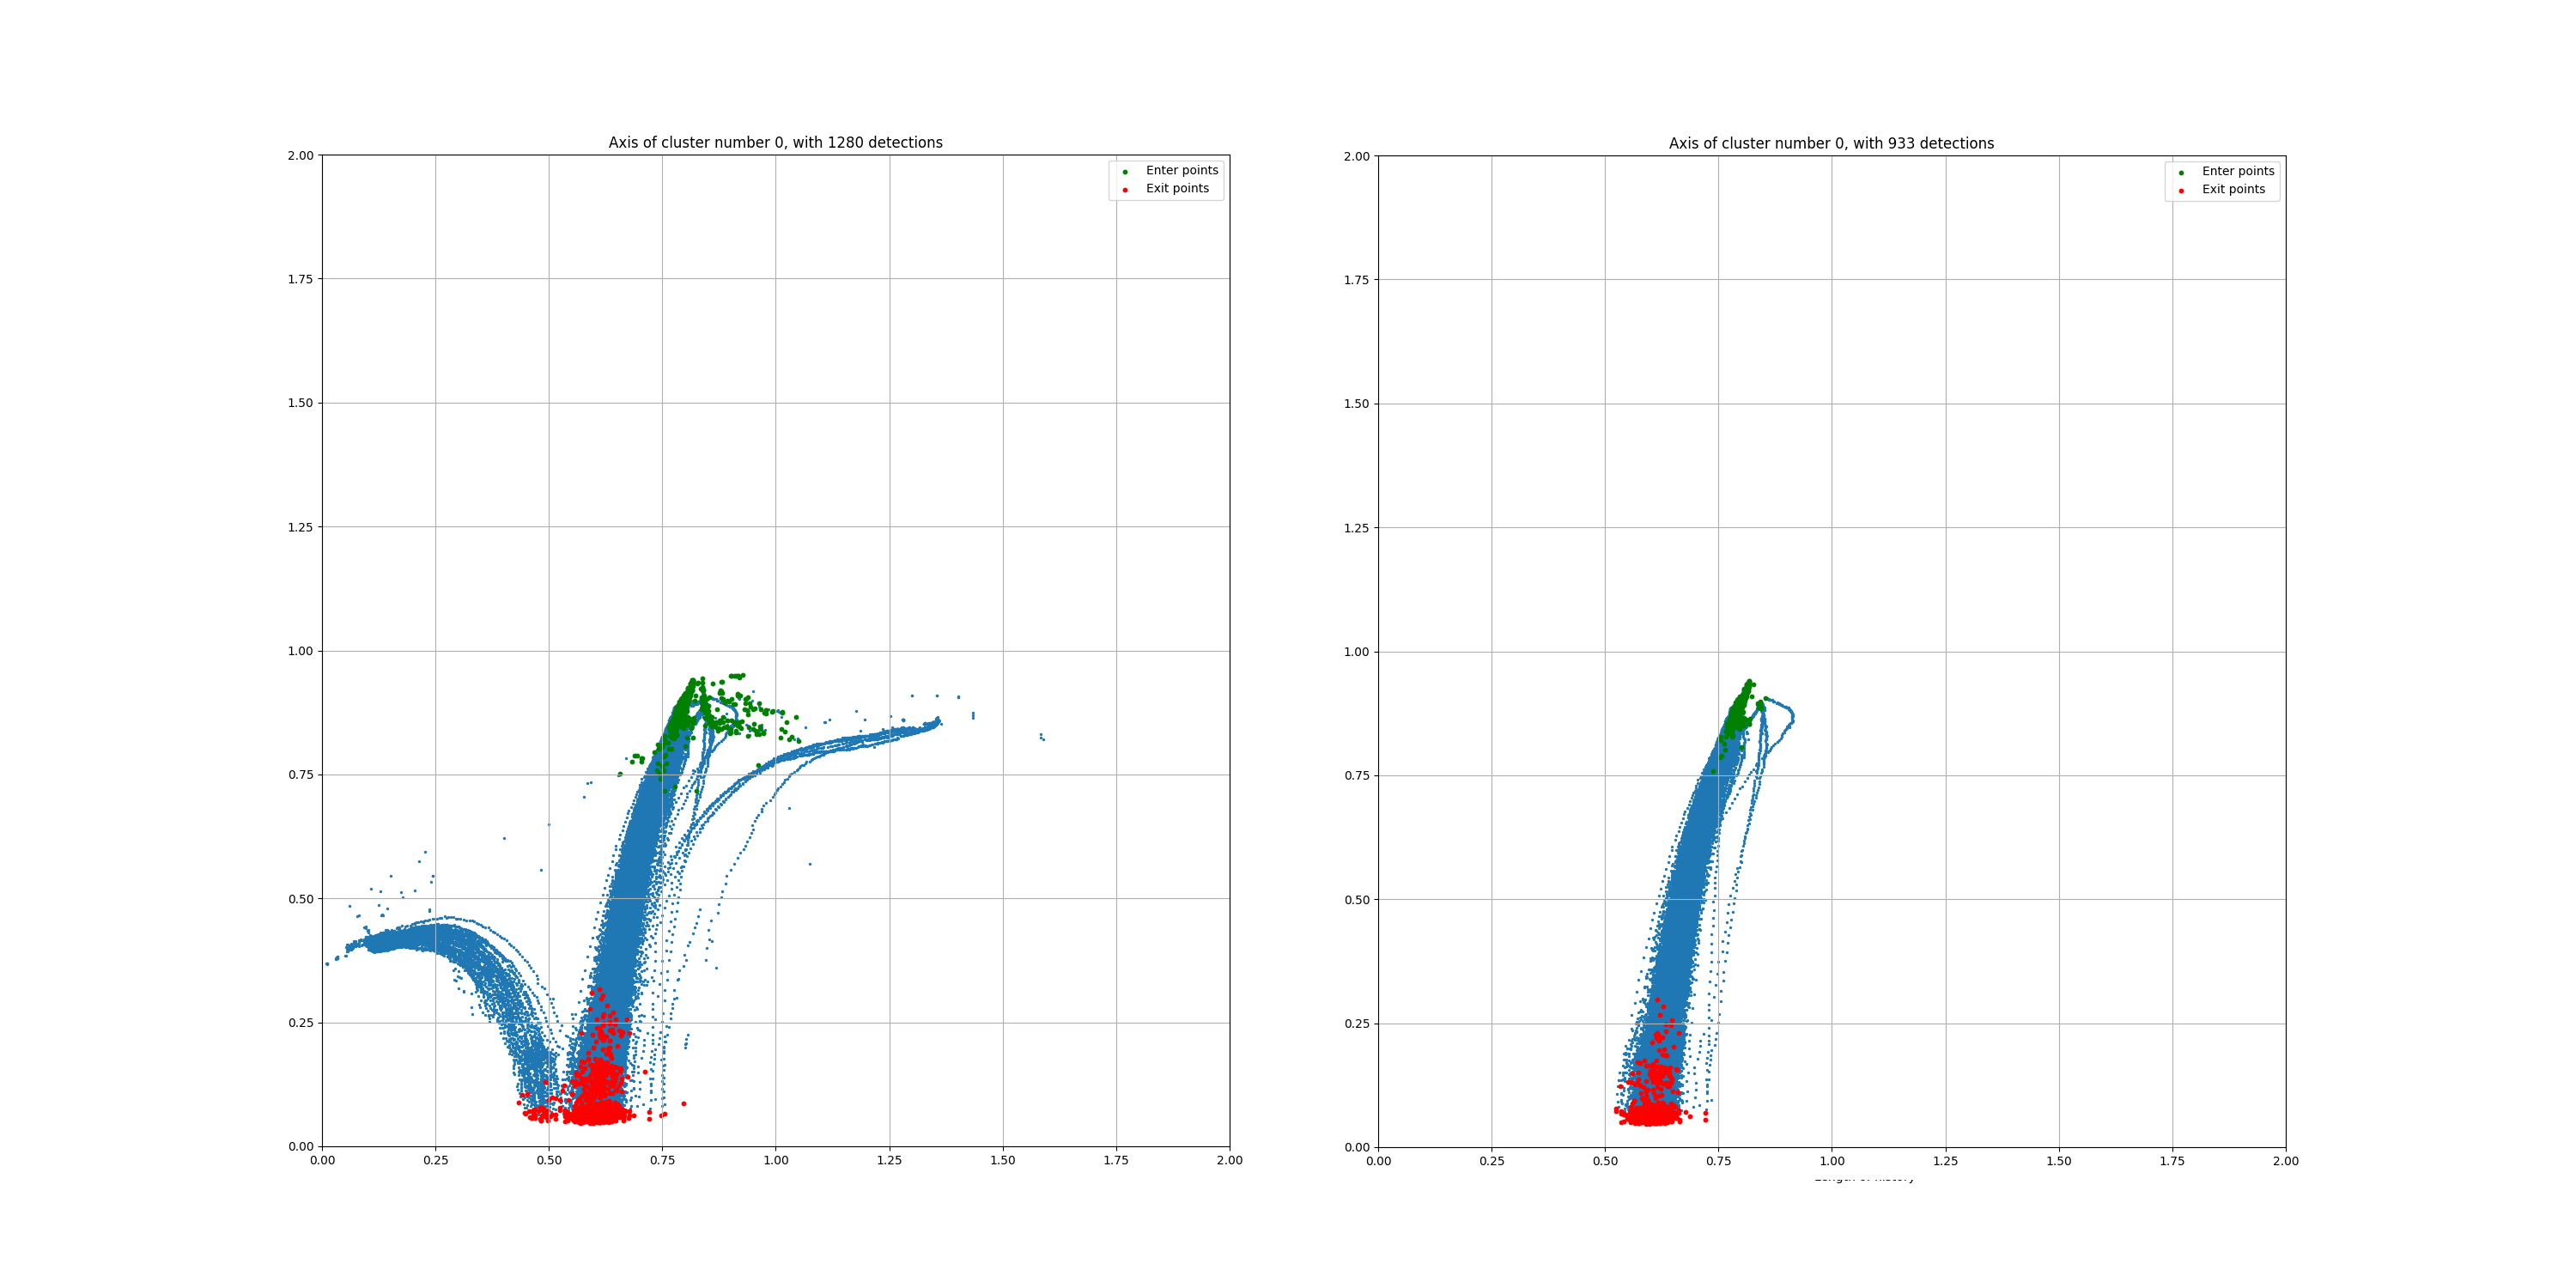
\includegraphics[width=0.8\columnwidth]{clustering/n_cluster_0_before_after.png}
    \centering
    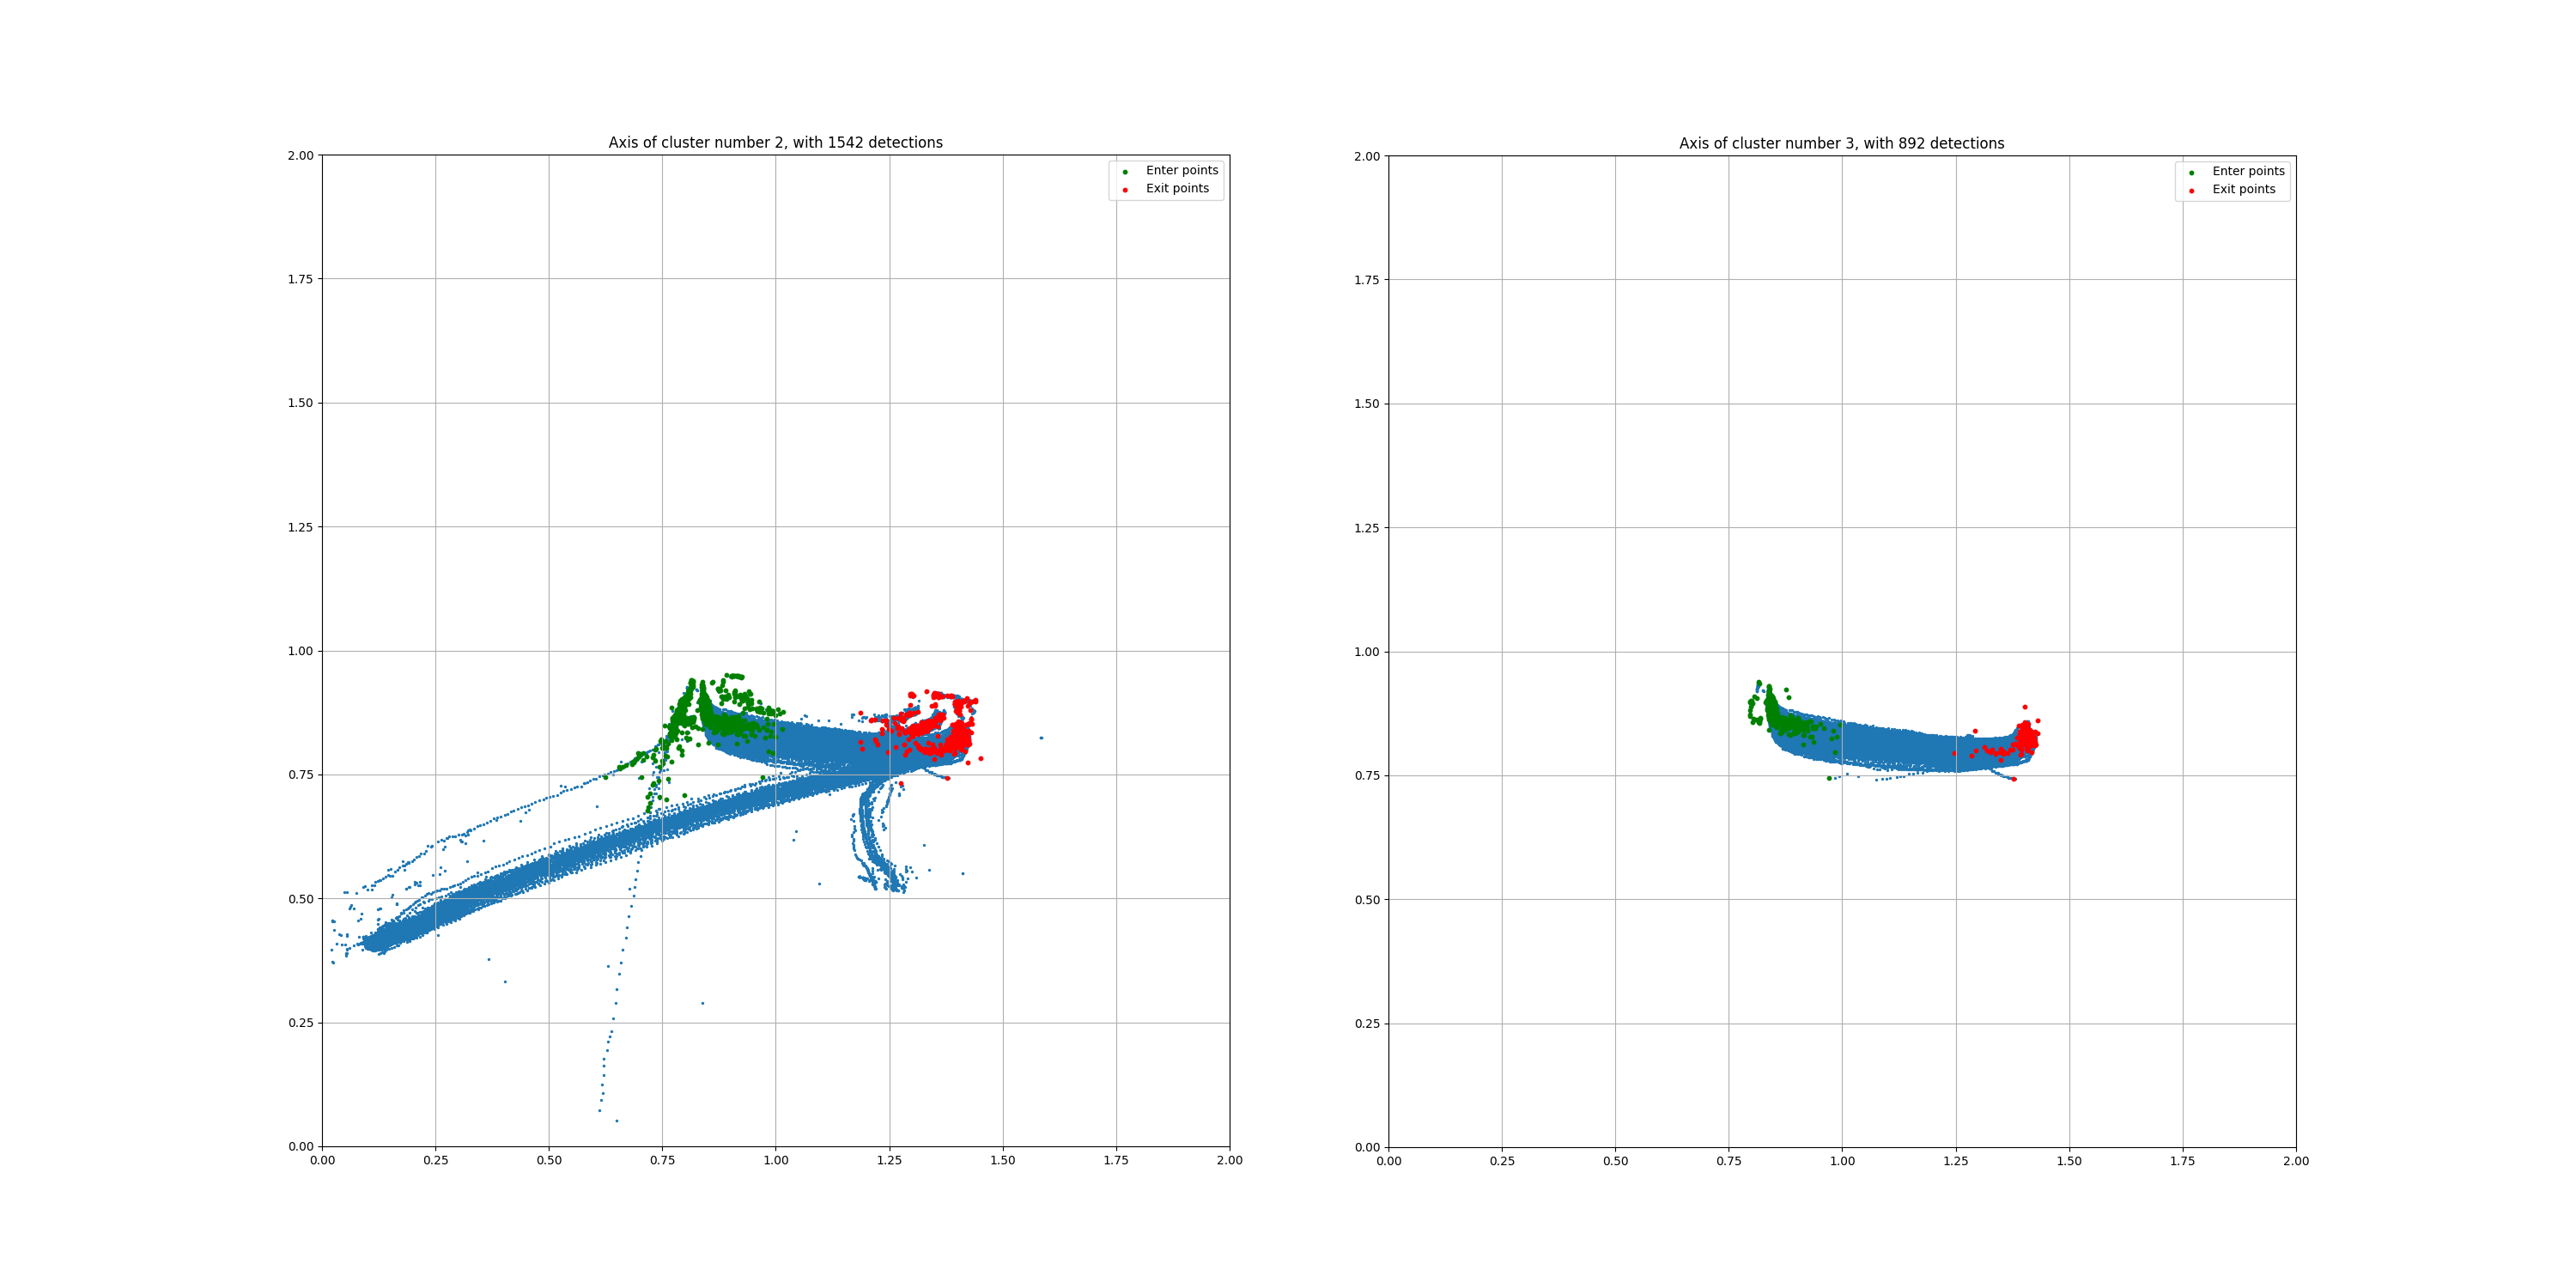
\includegraphics[width=0.8\columnwidth]{clustering/n_cluster_2_before_after.png}
    \caption{Klaszterezés szűrő (piros: kilépő pont, zöld: belépő pont)}
    \label{fig: Klaszterezés szűrő}
\end{figure}
\begin{figure}[htbp]
    \centering
    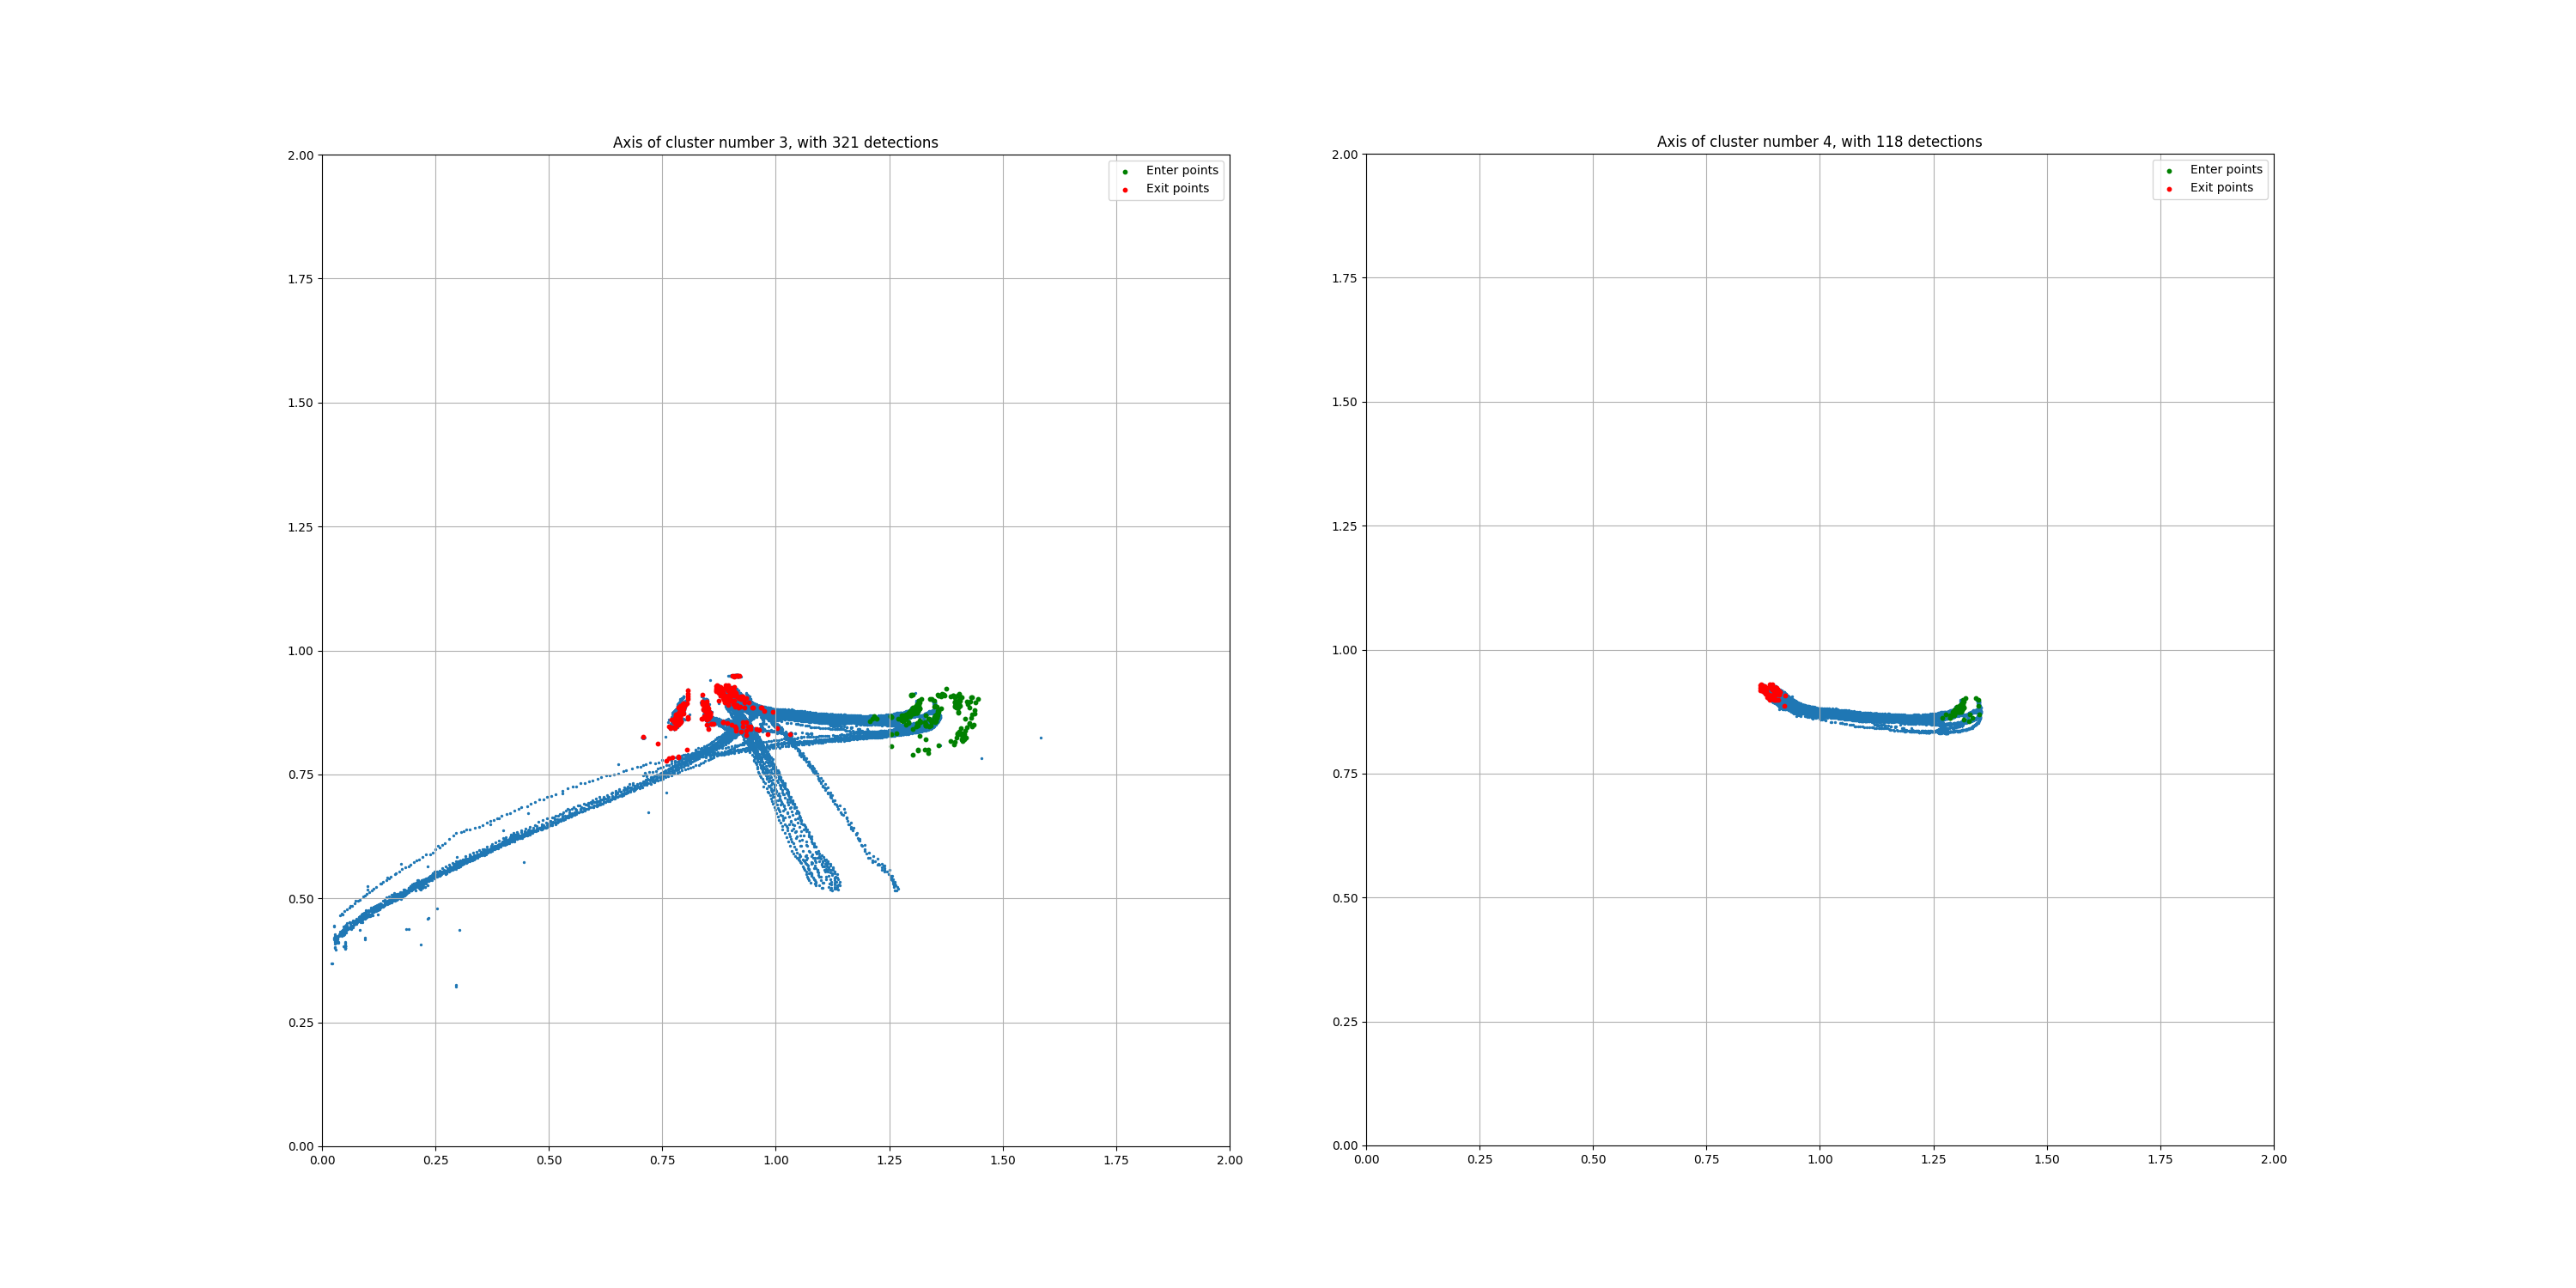
\includegraphics[width=0.8\columnwidth]{clustering/n_cluster_3_before_after.png}
    \centering
    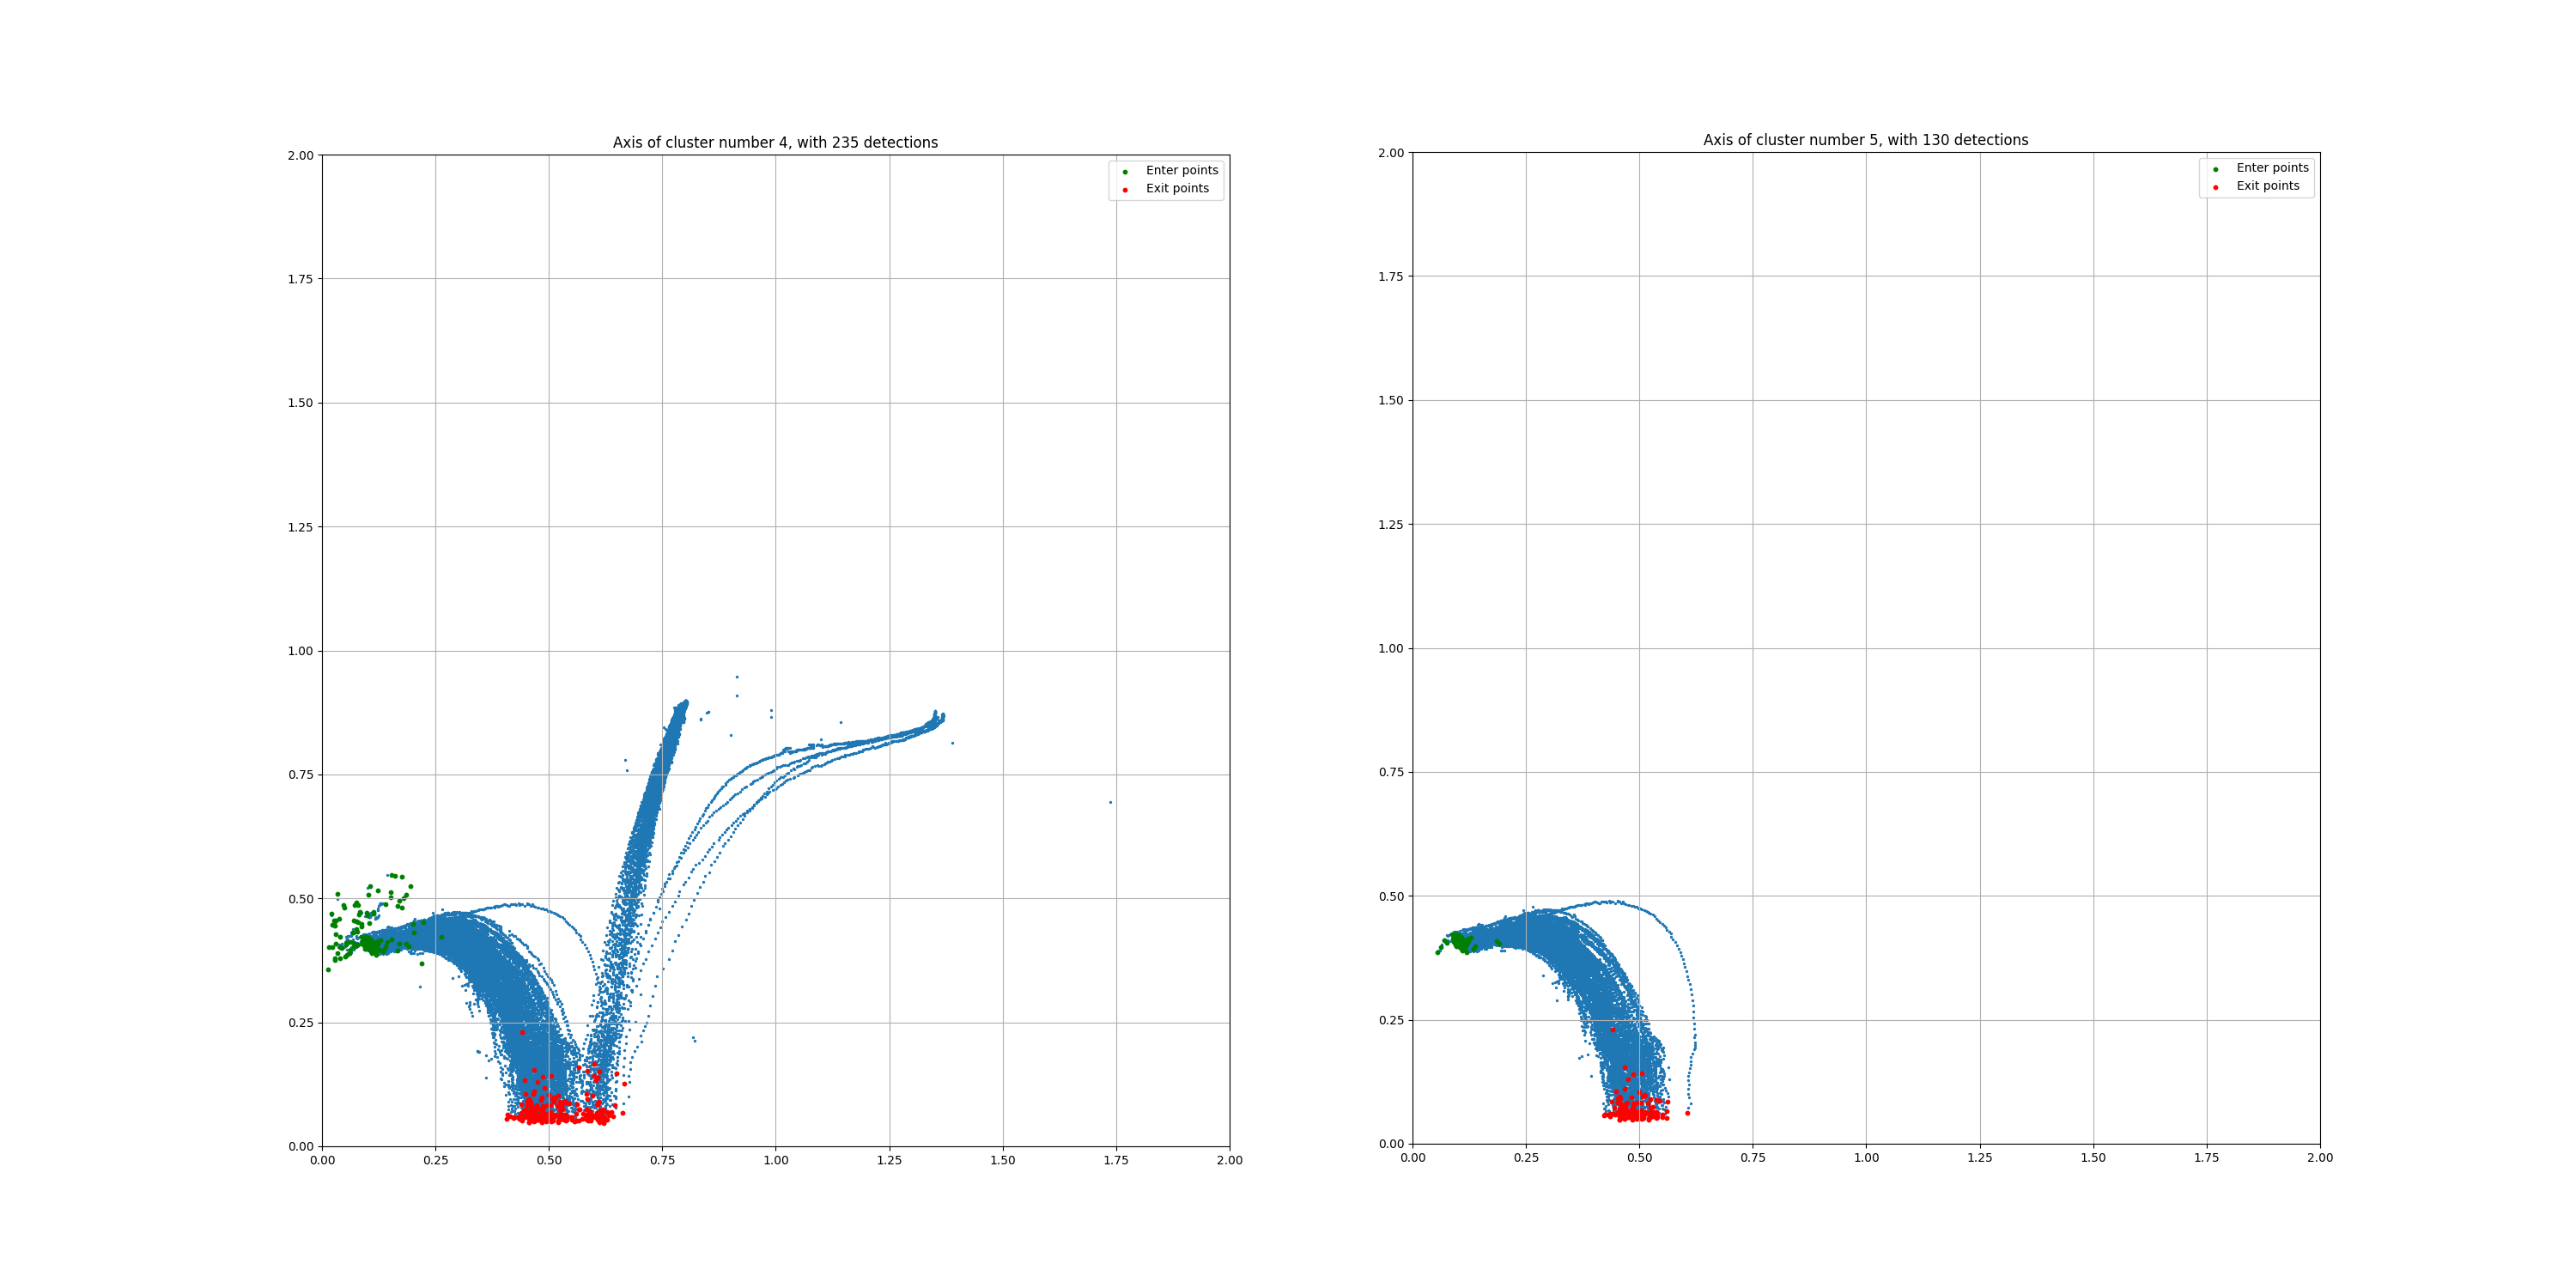
\includegraphics[width=0.8\columnwidth]{clustering/n_cluster_4_before_after.png}
    \centering
    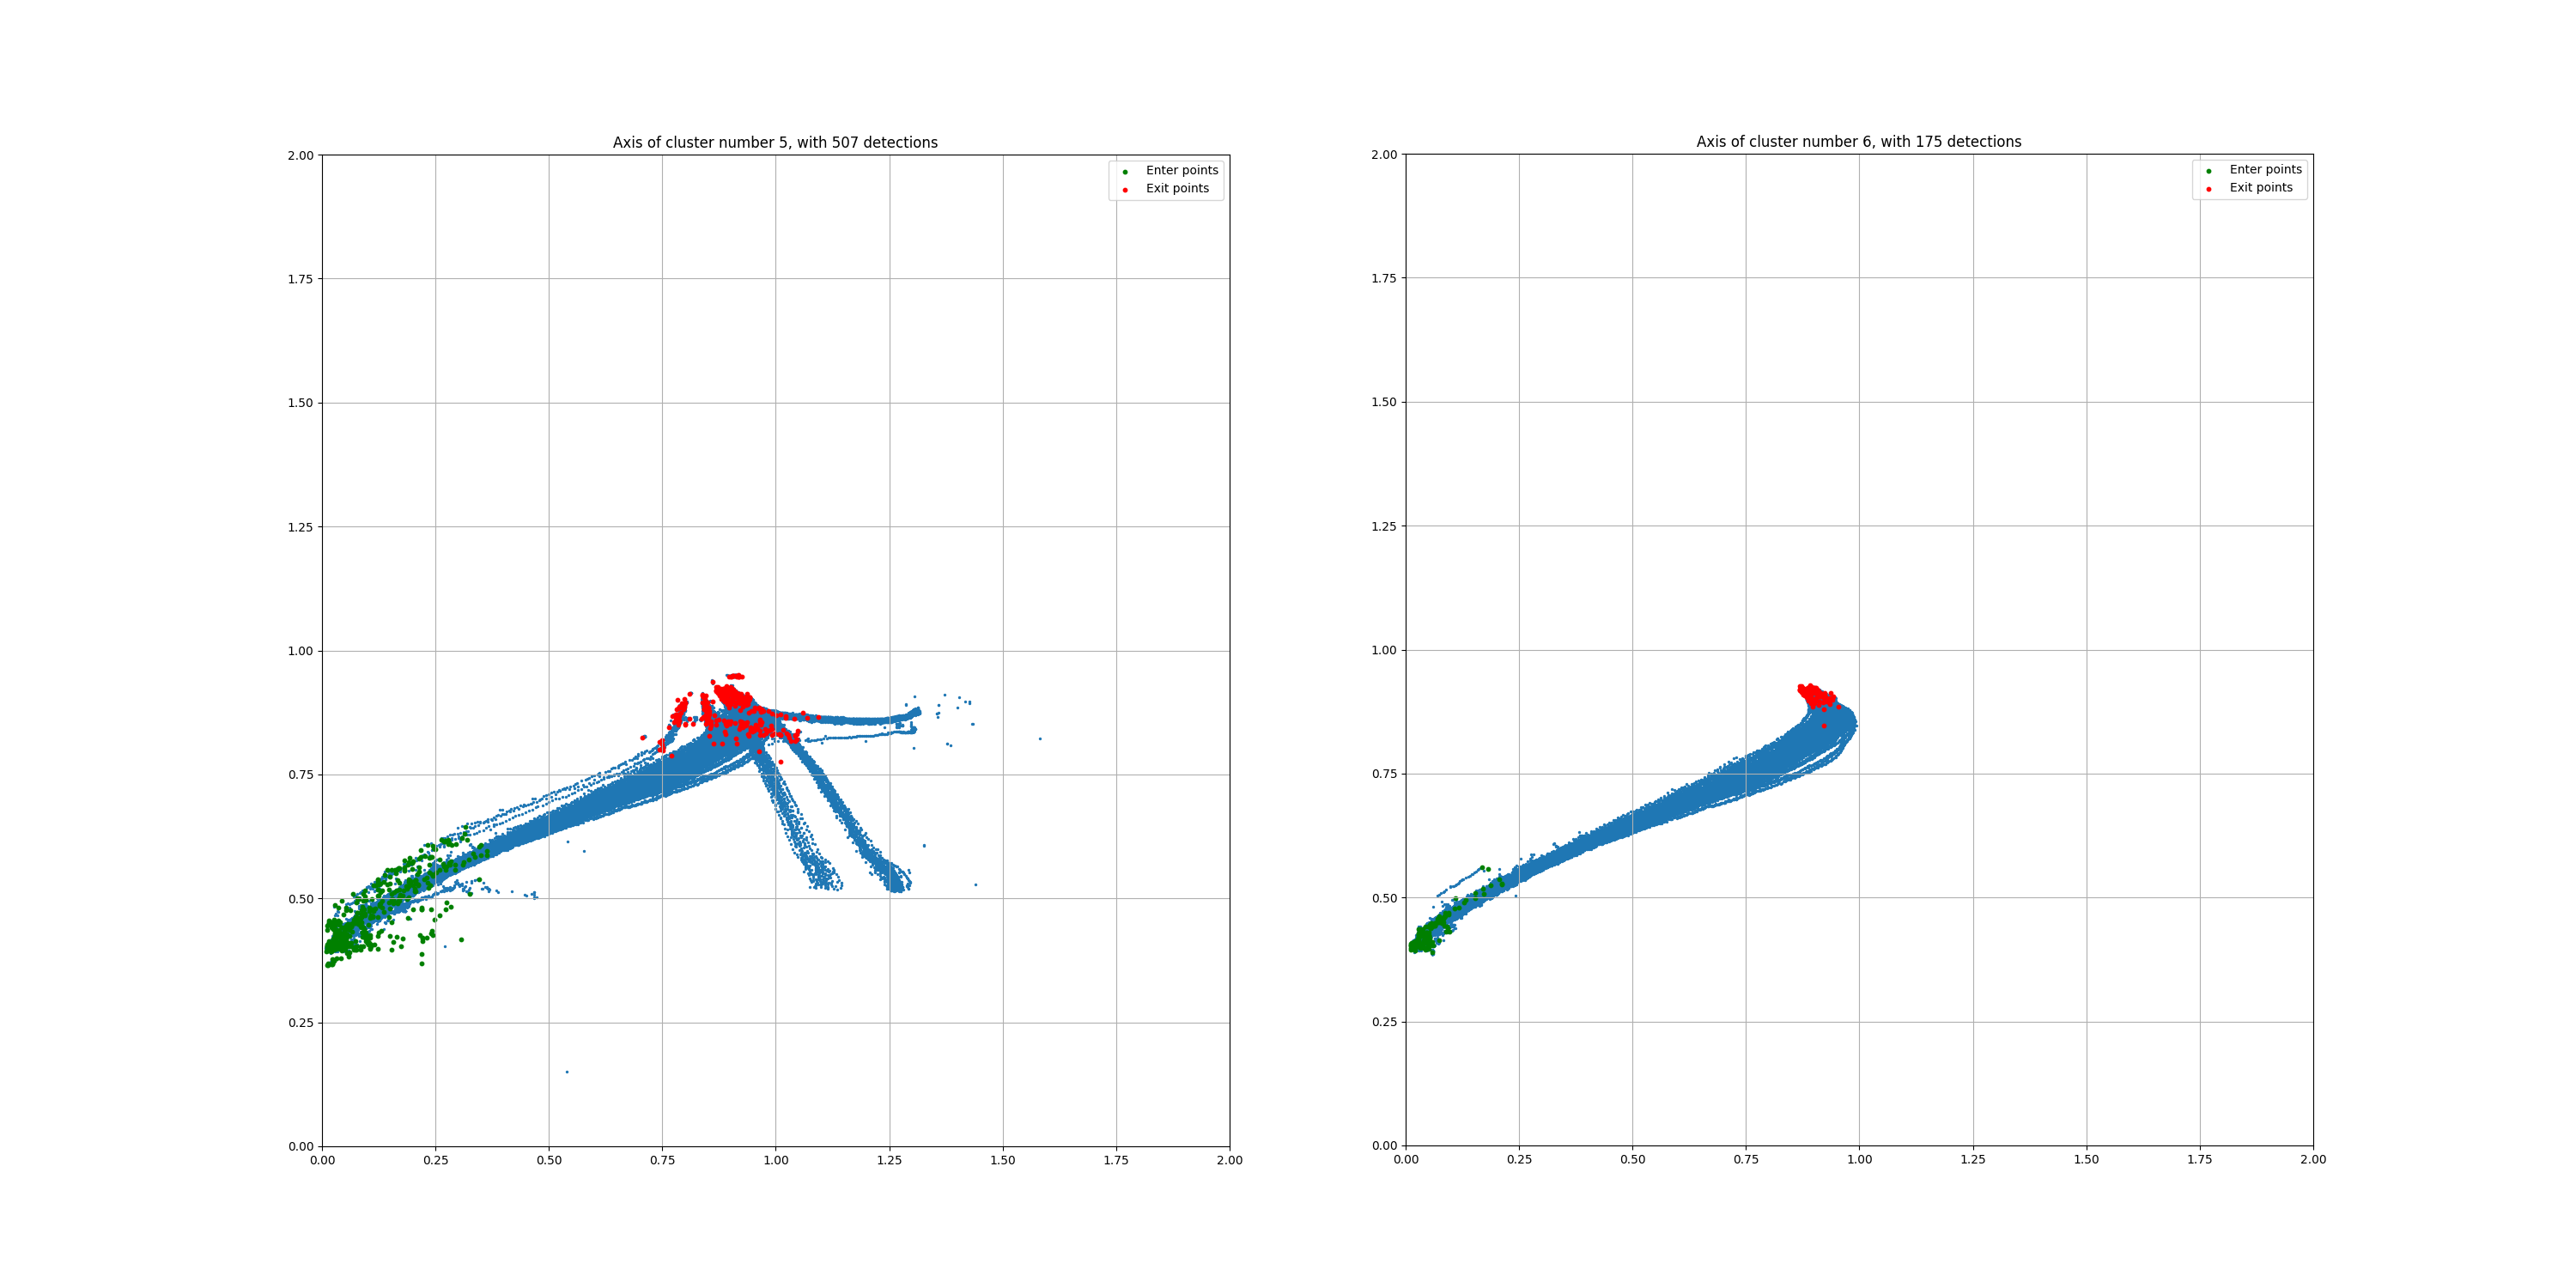
\includegraphics[width=0.8\columnwidth]{clustering/n_cluster_5_before_after.png}
    \caption{Klaszterezés szűrő}
    \label{fig: Klaszterezés szűrő2}
\end{figure}
\begin{figure}[htbp]
    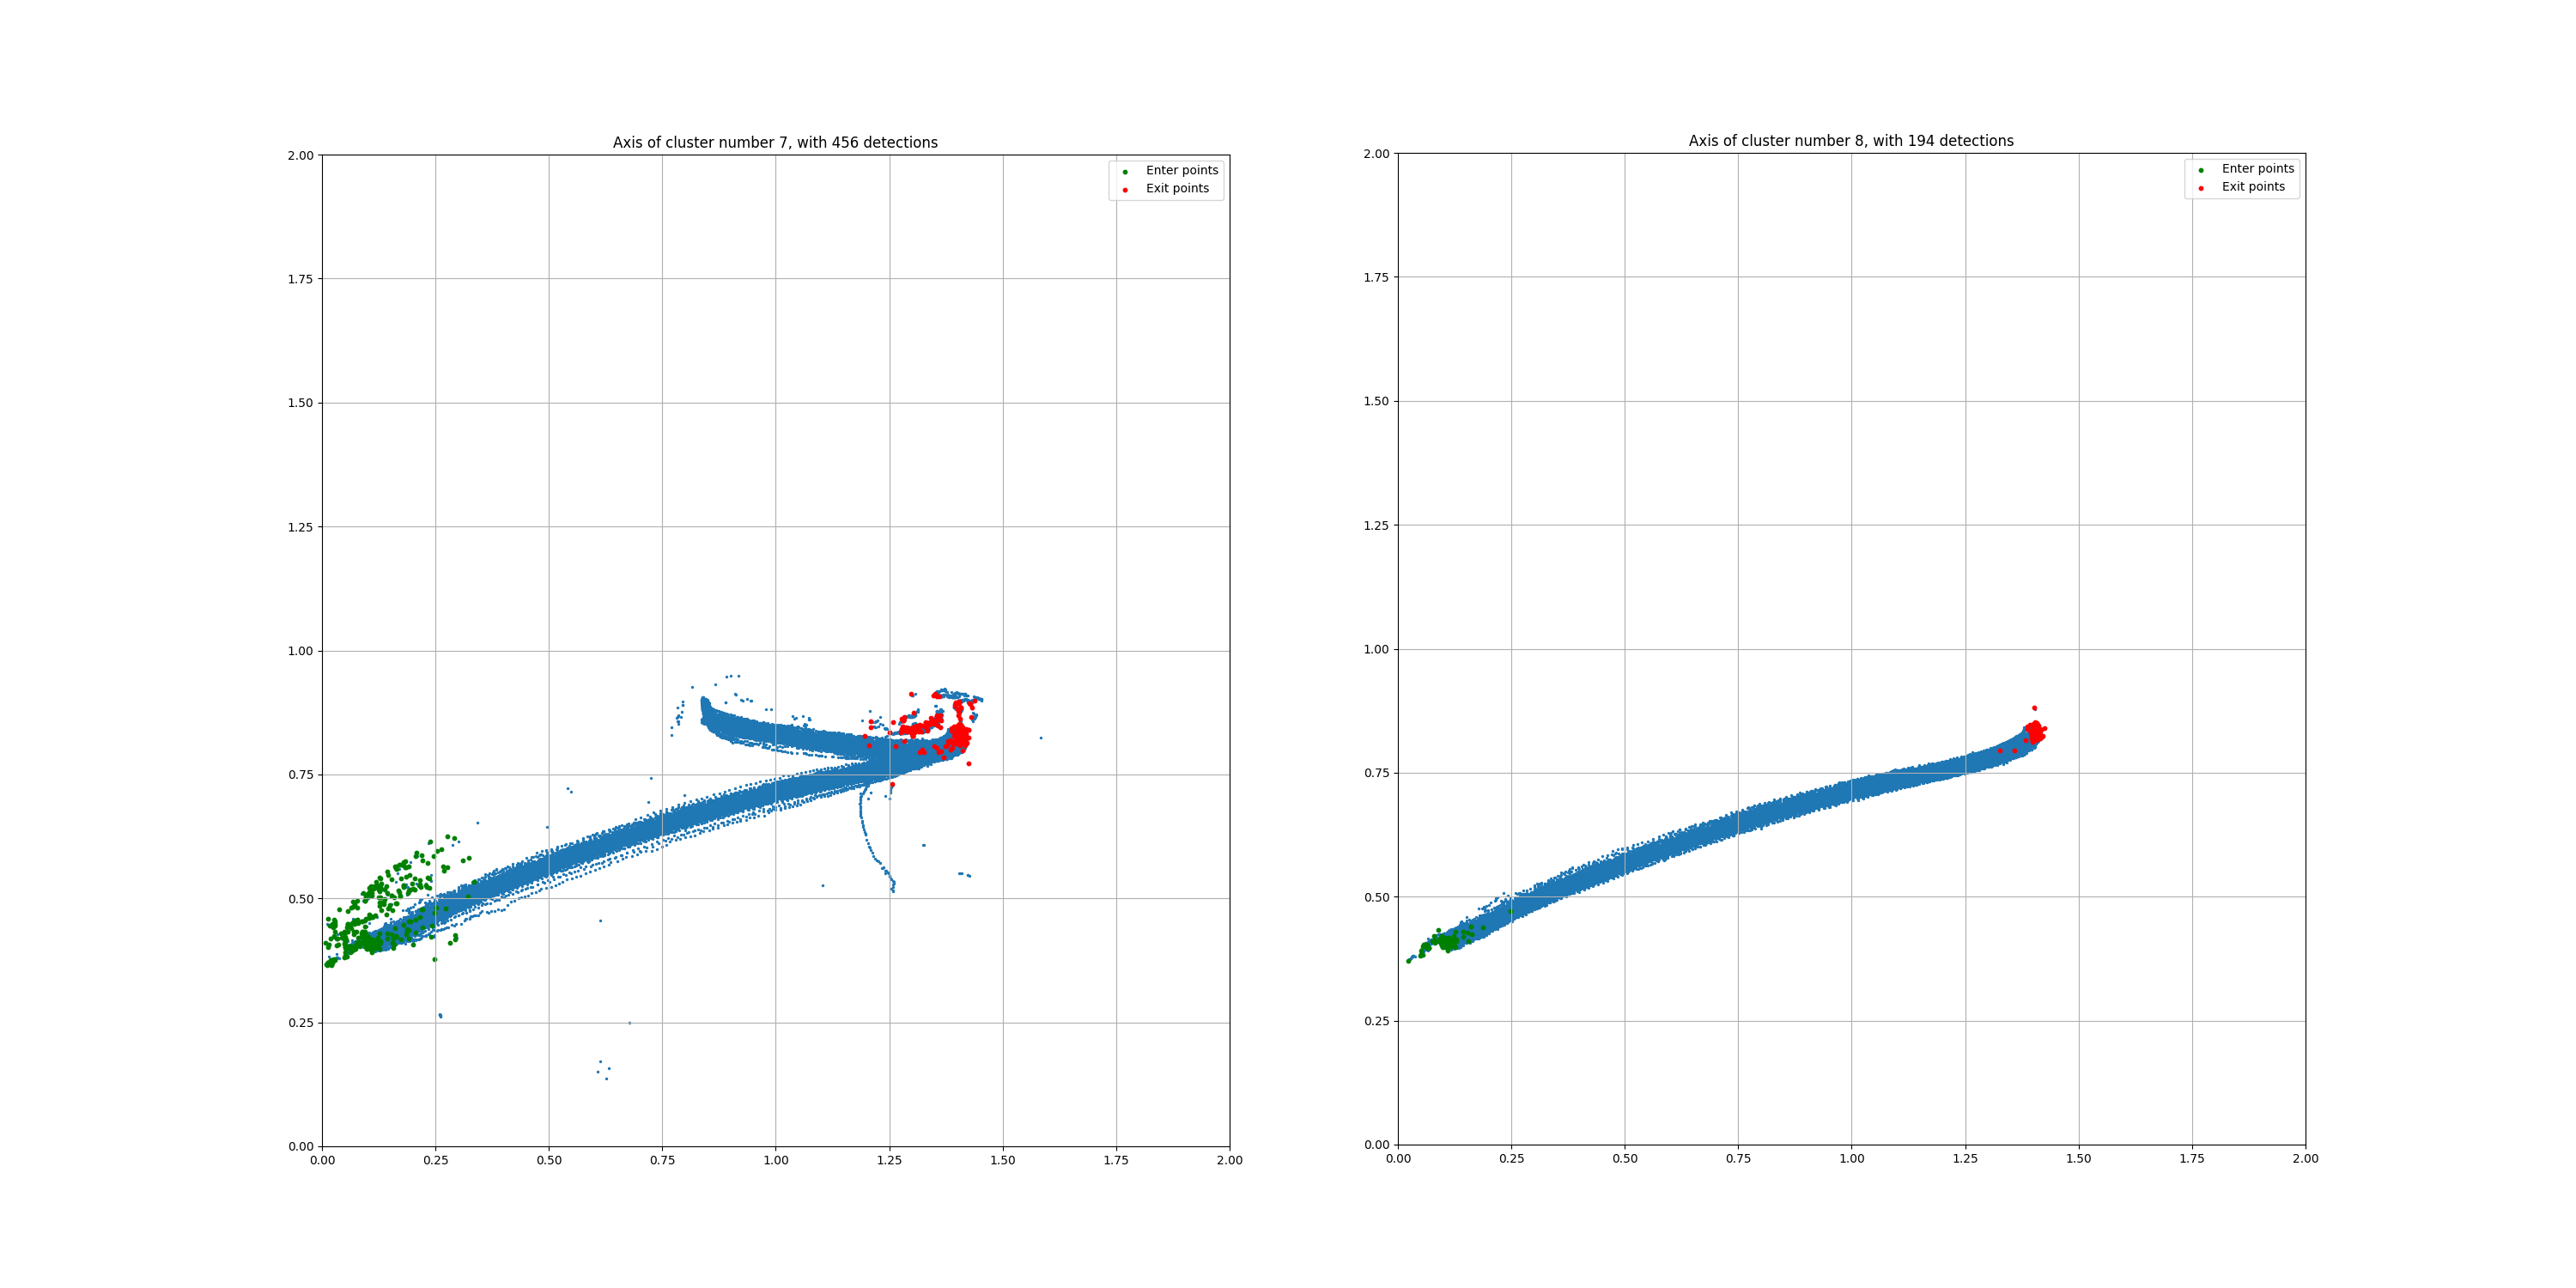
\includegraphics[width=1\columnwidth]{clustering/n_cluster_7_before_after.png}
    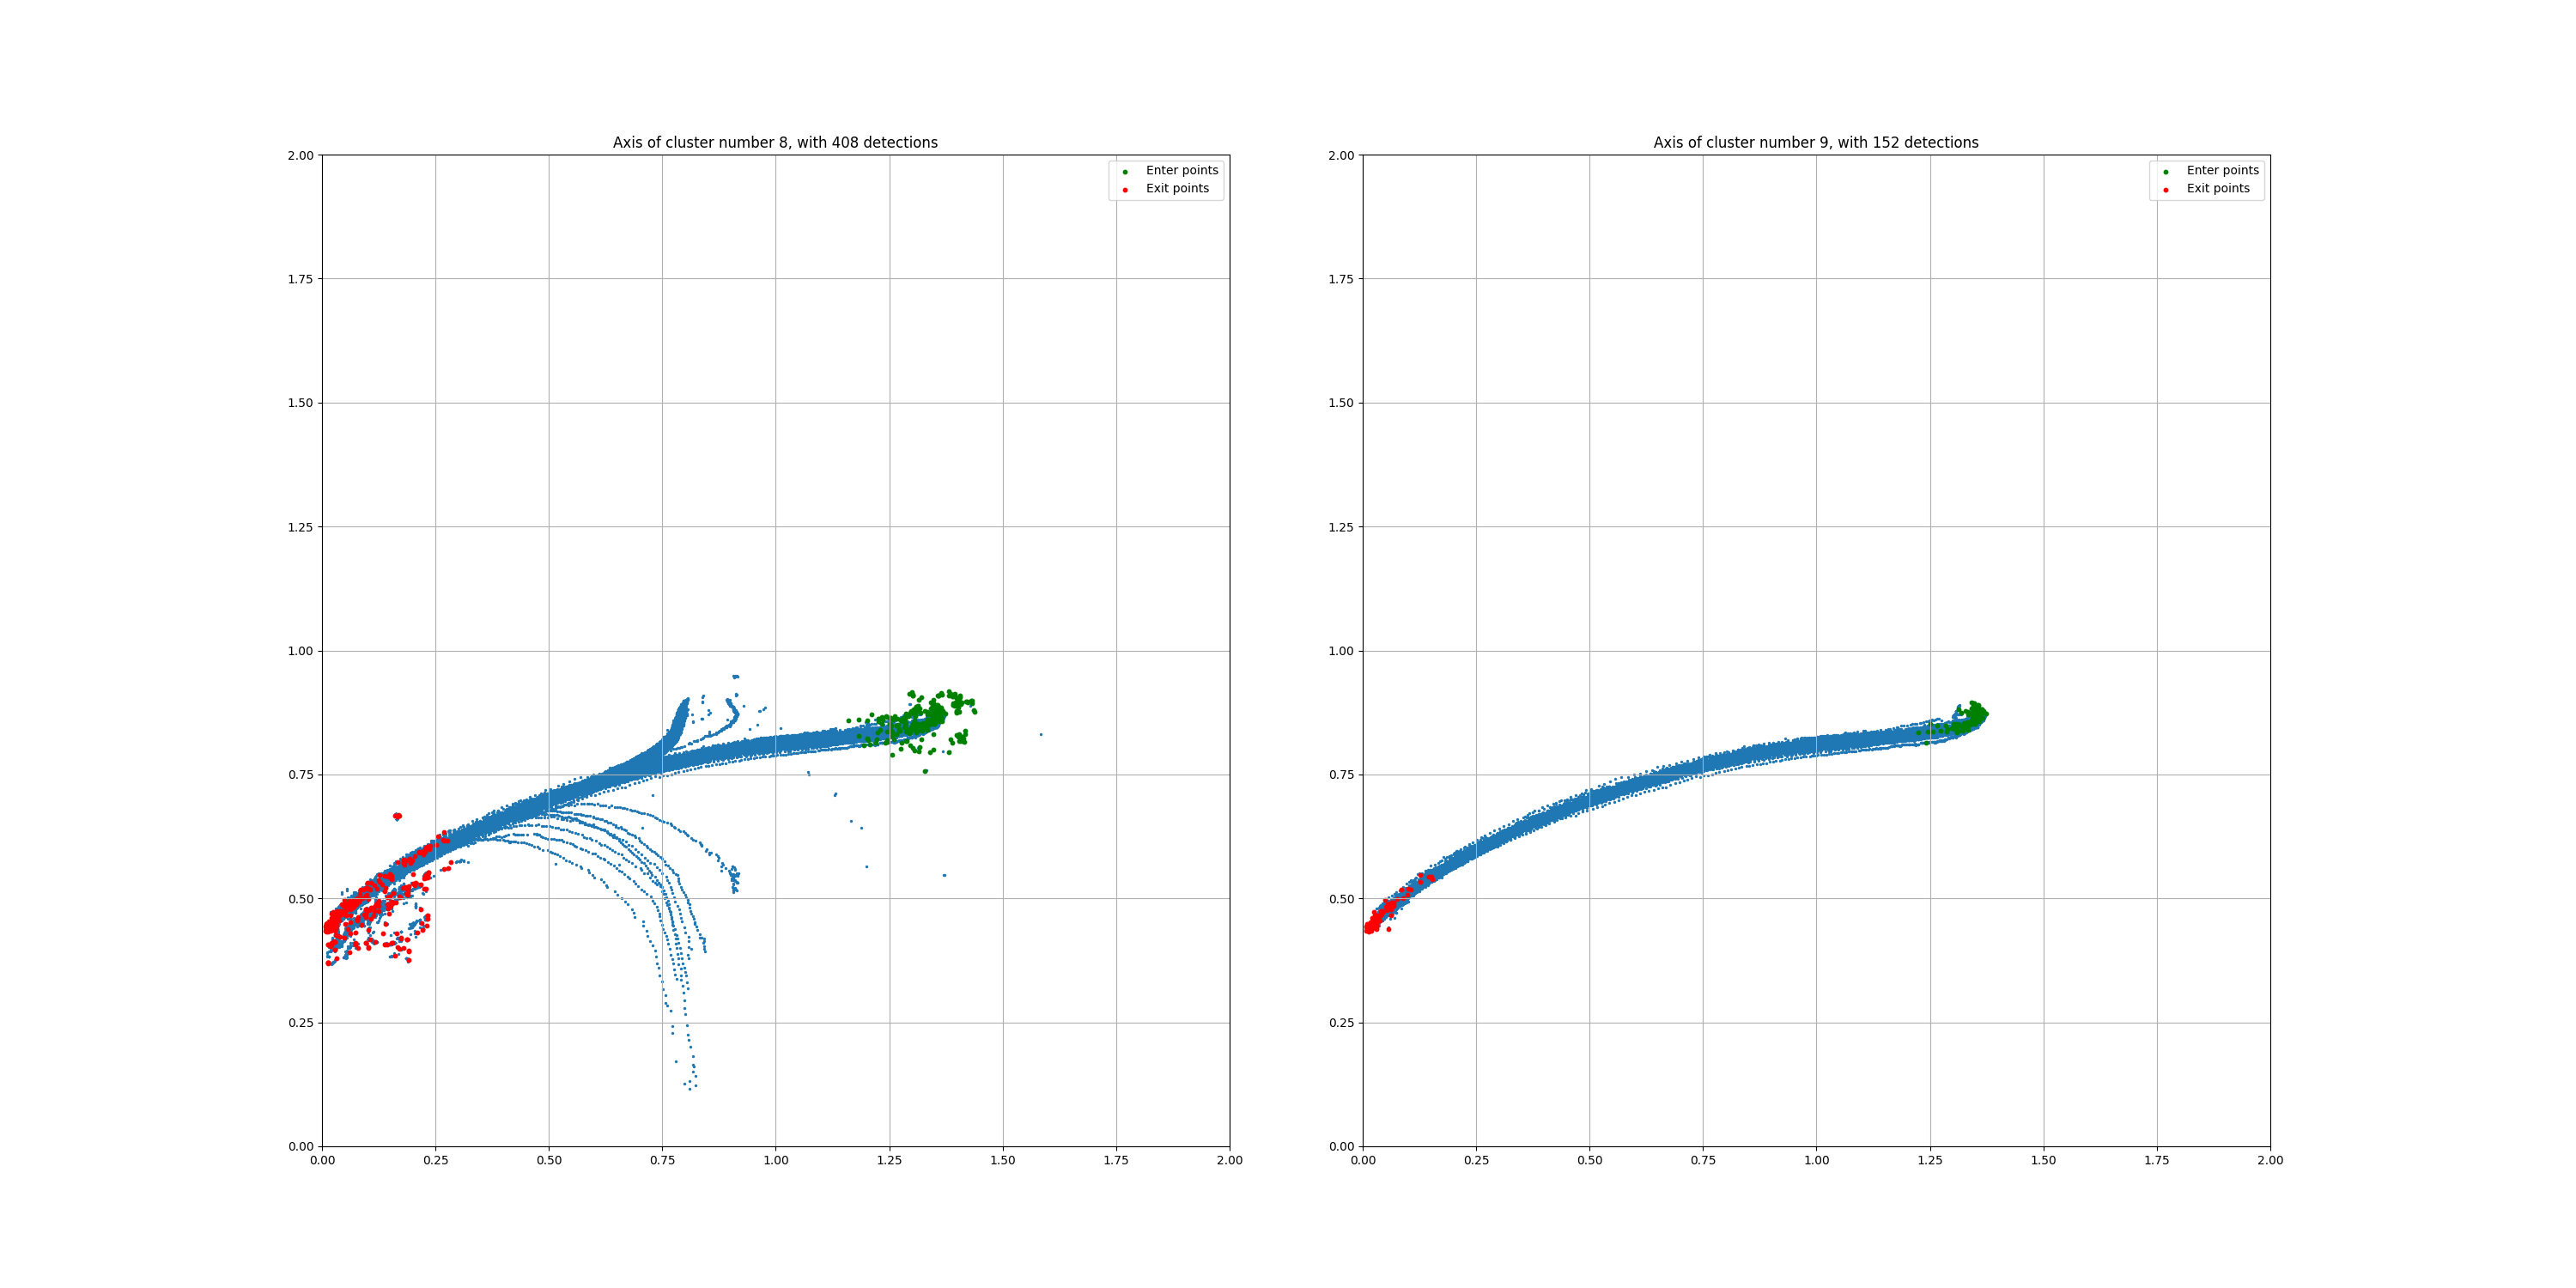
\includegraphics[width=1\columnwidth]{clustering/n_cluster_8_before_after.png}
    \caption{Klaszterezés szűrő}
    \label{fig: Klaszterezés szűrő3}
\end{figure}

\subsubsection{Yolov7 paraméterek}
A Yolo-nak főbb paraméterei a konfidencia és az IoU (Intersection over Union). A konfidencia azt jelenti, hogy a neurális hálózat mennyire biztos abban, hogy az adott objektumot azonosította.
Az IoU pedig azt jelenti, hogy a neurális hálózat mennyire biztos az objektum helyzetében. Ezen paraméterek finomhangolásával is javítani lehet a zajos detektálásokon és trajektóriákon.

\subsection{Feature vektorok}
Klaszterezéshez 4 és 6 dimenziós feature vektorokat használ-tunk. A 6 dimenziós vektorokat a DeepSORT hibájának a kiszűrésére hoztuk létre, felépítésük a következő [belépő x,y középső x,y kilépő x,y], de a kifejlesztett szűrők hatékonyabbaknak bizonyult, és a kevesebb dimenzió is előnyt jelent, ezért maradtunk a 4 dimenziós feature vektor mellett, aminek a felépítése: [belépő x,y kilépő x,y].
\subsection{Klaszterezési algoritmusok}
Klaszterezéshez több fajta algoritmust teszteltünk. A legjobb eredményeket az OPTICS (Ordering Points To Identify the Clustering Structure) \cite{10.1145/304181.304187} algoritmus adta.
Aminek az eredményei a fenti képeken látható (lásd. \ref{fig: Bad clusters}). A képen bal oldalon láthatók rendre a KMeans, DBSCAN és BIRCH által rendezett klaszterek, a jobb oldalon pedig az OPTICS által rendezett klaszterek. Az utolsó sorban a BIRCH eredménye látható, ahol két klasztert egybevont, amit az OPTICS meg tudott különböztetni.
OPTICS-on kívül teszteltük a KMeans, DBSCAN és BIRCH algoritmusokat.
\paragraph{KMeans} A KMeans klaszterezés egy unsupervised machine learning algoritmus, amely célja az adatok csoportosítása oly módon, hogy azonos klaszterbe tartozó adatok közötti távolság minimális legyen, míg az eltérő klaszterek közötti távolság maximális.
Az algoritmus működése a következő lépésekből áll:
\begin{enumerate}
    \item Centroidok inicializálása: Az algoritmus véletlenszerűen inicializál k centroidot a dataseten, ahol k a klaszterek száma.
    \item Adatok csoportosítása: Az algoritmus minden adatponthoz hozzárendeli a legközelebbi centroidot, és azonos klaszterbe helyezi azokat az adatpontokat, amelyeknek a centroidja megegyezik.
    \item Centroidok újraszámolása: Az algoritmus újraszámolja a centroidok pozícióit az adatok csoportosítása után, hogy azok a klaszterben található adatpontok átlagértékének megfelelően helyezkedjenek el.
    \item Lépések ismétlése: Az algoritmus addig ismételgeti a 2. és 3. lépéseket, amíg az adatpontok klaszterezése konvergens állapotba nem jut, azaz az adatpontok csoportosítása már nem változik, vagy az algoritmus előre meghatározott maximális iterációs számhoz ér.
    \item Klaszterek értékelése: Az algoritmus kiértékeli a klaszterek minőségét, például a csoportokban lévő adatpontok közötti távolságot, és eldönti, hogy a csoportokat újra kell-e szervezni.
\end{enumerate}
A KMeans klaszterezés előnye, hogy egyszerű és gyors algoritmus, amely hatékonyan használható az adatok csoportosítására. A klaszterek számát könnyen meg lehet adni, és az algoritmus gyorsan konvergál. Azonban az algoritmus érzékeny az inicializálási folyamatokra, és gyakran találhatók olyan csoportok, amelyek nem teljesen homogének.
Emellett KMeans $n\_clusters$ - klaszterek száma - paraméterét előre kell definiálni, aminek meghatározására próbálkoztunk különböző metrikákat felhasználni, hogy automatizálható legyen
a klaszterezési lépés. Ezek a metrikák a Silhouette Coefficient \cite{ROUSSEEUW198753}, Calinski-Harabasz Index \cite{10.1080/03610927408827101} és Davies-Bouldin Index \cite{4766909}.
Elbow diagramok segítségével próbáltuk eldönteni, hogy milyen értéket érdemes adni az \begin{math}n\_clusters\end{math} paraméternek lásd \ref{fig: Elbow diagramok}.
A mérőszámok konzisztensen alacsony értéket adtak, egy négyágú kereszteződésnél, ahol jóval több klaszterbe sorolhatók a trajektóriák. A KMeans használatát
ezért elvetettük.

\begin{figure}[htbp]
    \centering
    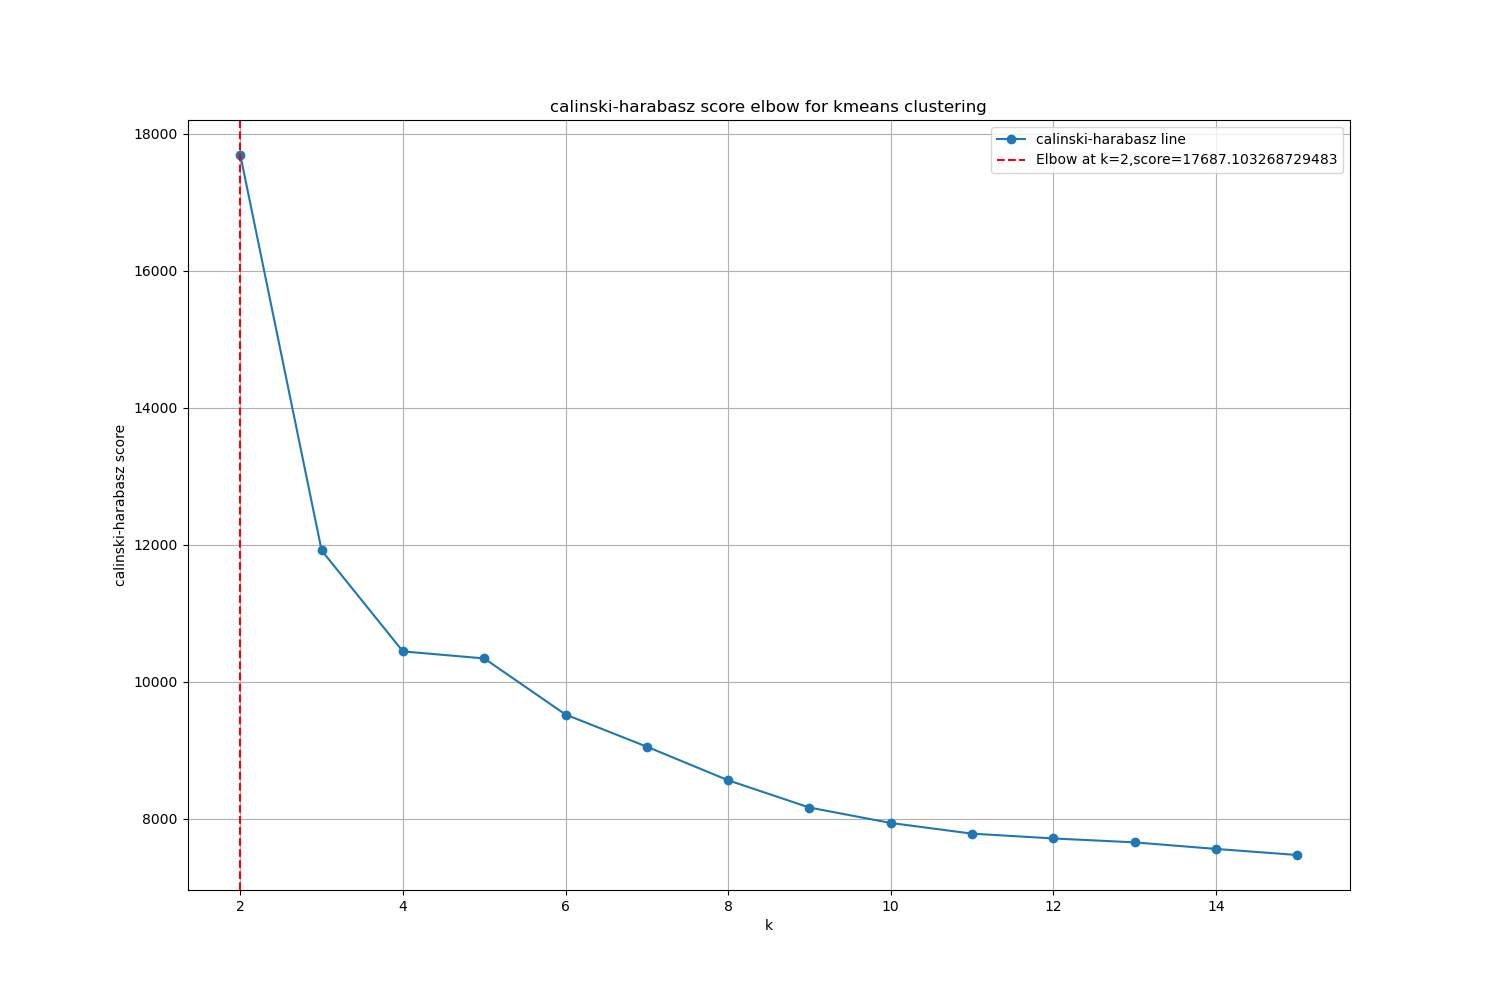
\includegraphics[width=0.7\columnwidth]{elbow/elbow_on_kmeans_2-16_metric_calinski-harabasz_thresh_0.5.png}
    \centering
    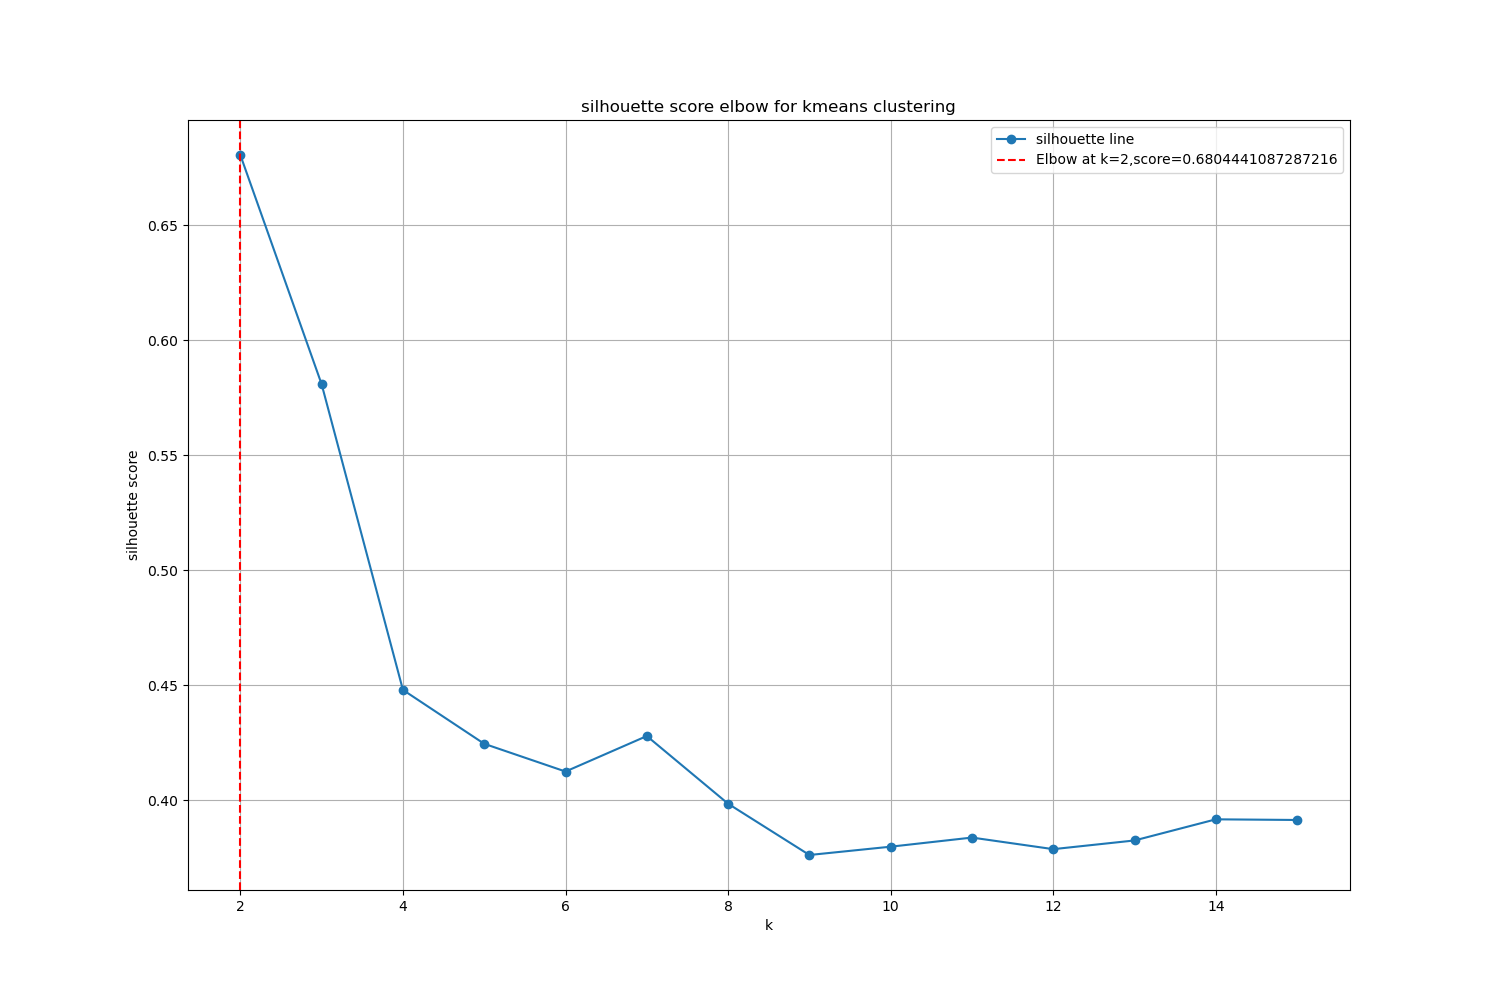
\includegraphics[width=0.7\columnwidth]{elbow/elbow_on_kmeans_2-16_metric_silhouette_thresh_0.5.png}
    \centering
    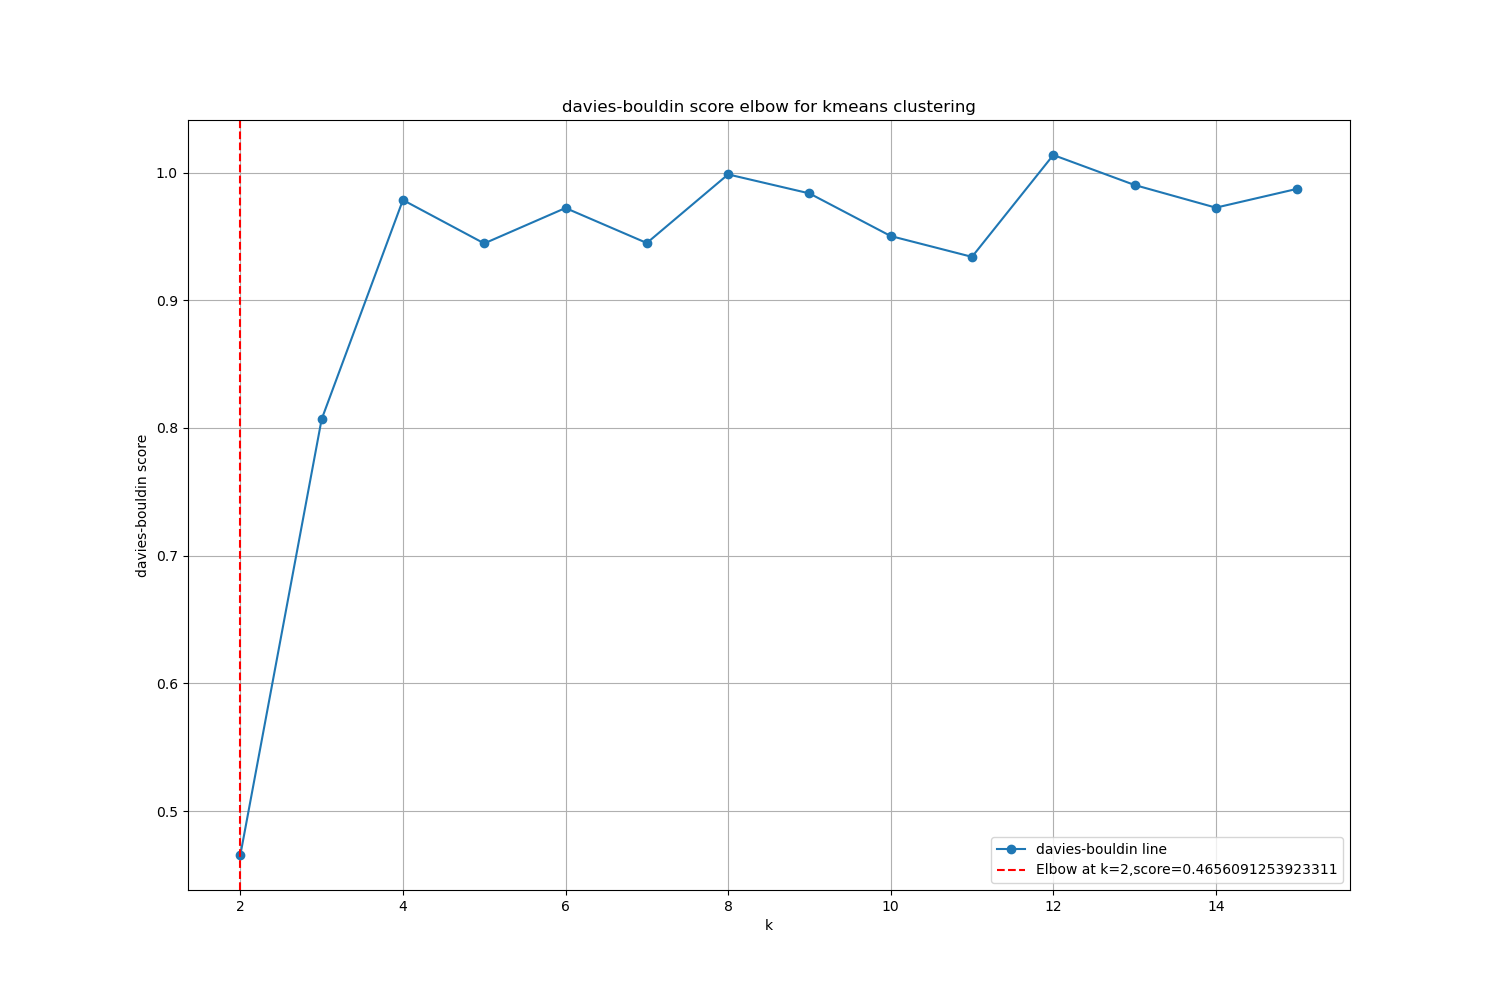
\includegraphics[width=0.68\columnwidth]{elbow/elbow_on_kmeans_2-16_metric_davies-bouldin_thresh_0.5.png}

    \caption{Elbow diagramok}
    \label{fig: Elbow diagramok}
\end{figure}

\begin{figure}[htbp]
    \begin{minipage}{.5\textwidth}
        \centering
        \includegraphics[width=1\linewidth]{KMeans/n_cluster_0_n_tracks_256.png}
        \caption{KMeans csoport}
        \label{fig:kmeans_cluster}
    \end{minipage}%
    \begin{minipage}{.5\textwidth}
        \centering
        \includegraphics[width=1\linewidth]{OPTICS/n_cluster_4_n_tracks_186.png}
        \caption{OPTICS csoport}
        \label{fig:optics_cluster}
    \end{minipage}
\end{figure}

\begin{figure}[htpb]
    \begin{minipage}{.5\textwidth}
        \centering
        \includegraphics[width=1\linewidth]{Birch/n_cluster_3_n_tracks_608.png}
        \caption{BIRCH csoport}
        \label{fig:birch_cluster}
    \end{minipage}%
    \begin{minipage}{.5\textwidth}
        \centering
        \includegraphics[width=1\linewidth]{OPTICS/n_cluster_4_n_tracks_186.png}
        \caption{OPTICS csoport alulról felfelé}
        \label{fig:optics_cluster_2}
        \includegraphics[width=1\linewidth]{OPTICS/n_cluster_1_n_tracks_587.png}
        \caption{OPTICS csoport jobbról balra}
        \label{fig:optics_cluster_3}
    \end{minipage}
\end{figure}

% \begin{figure}
%     \centering
%     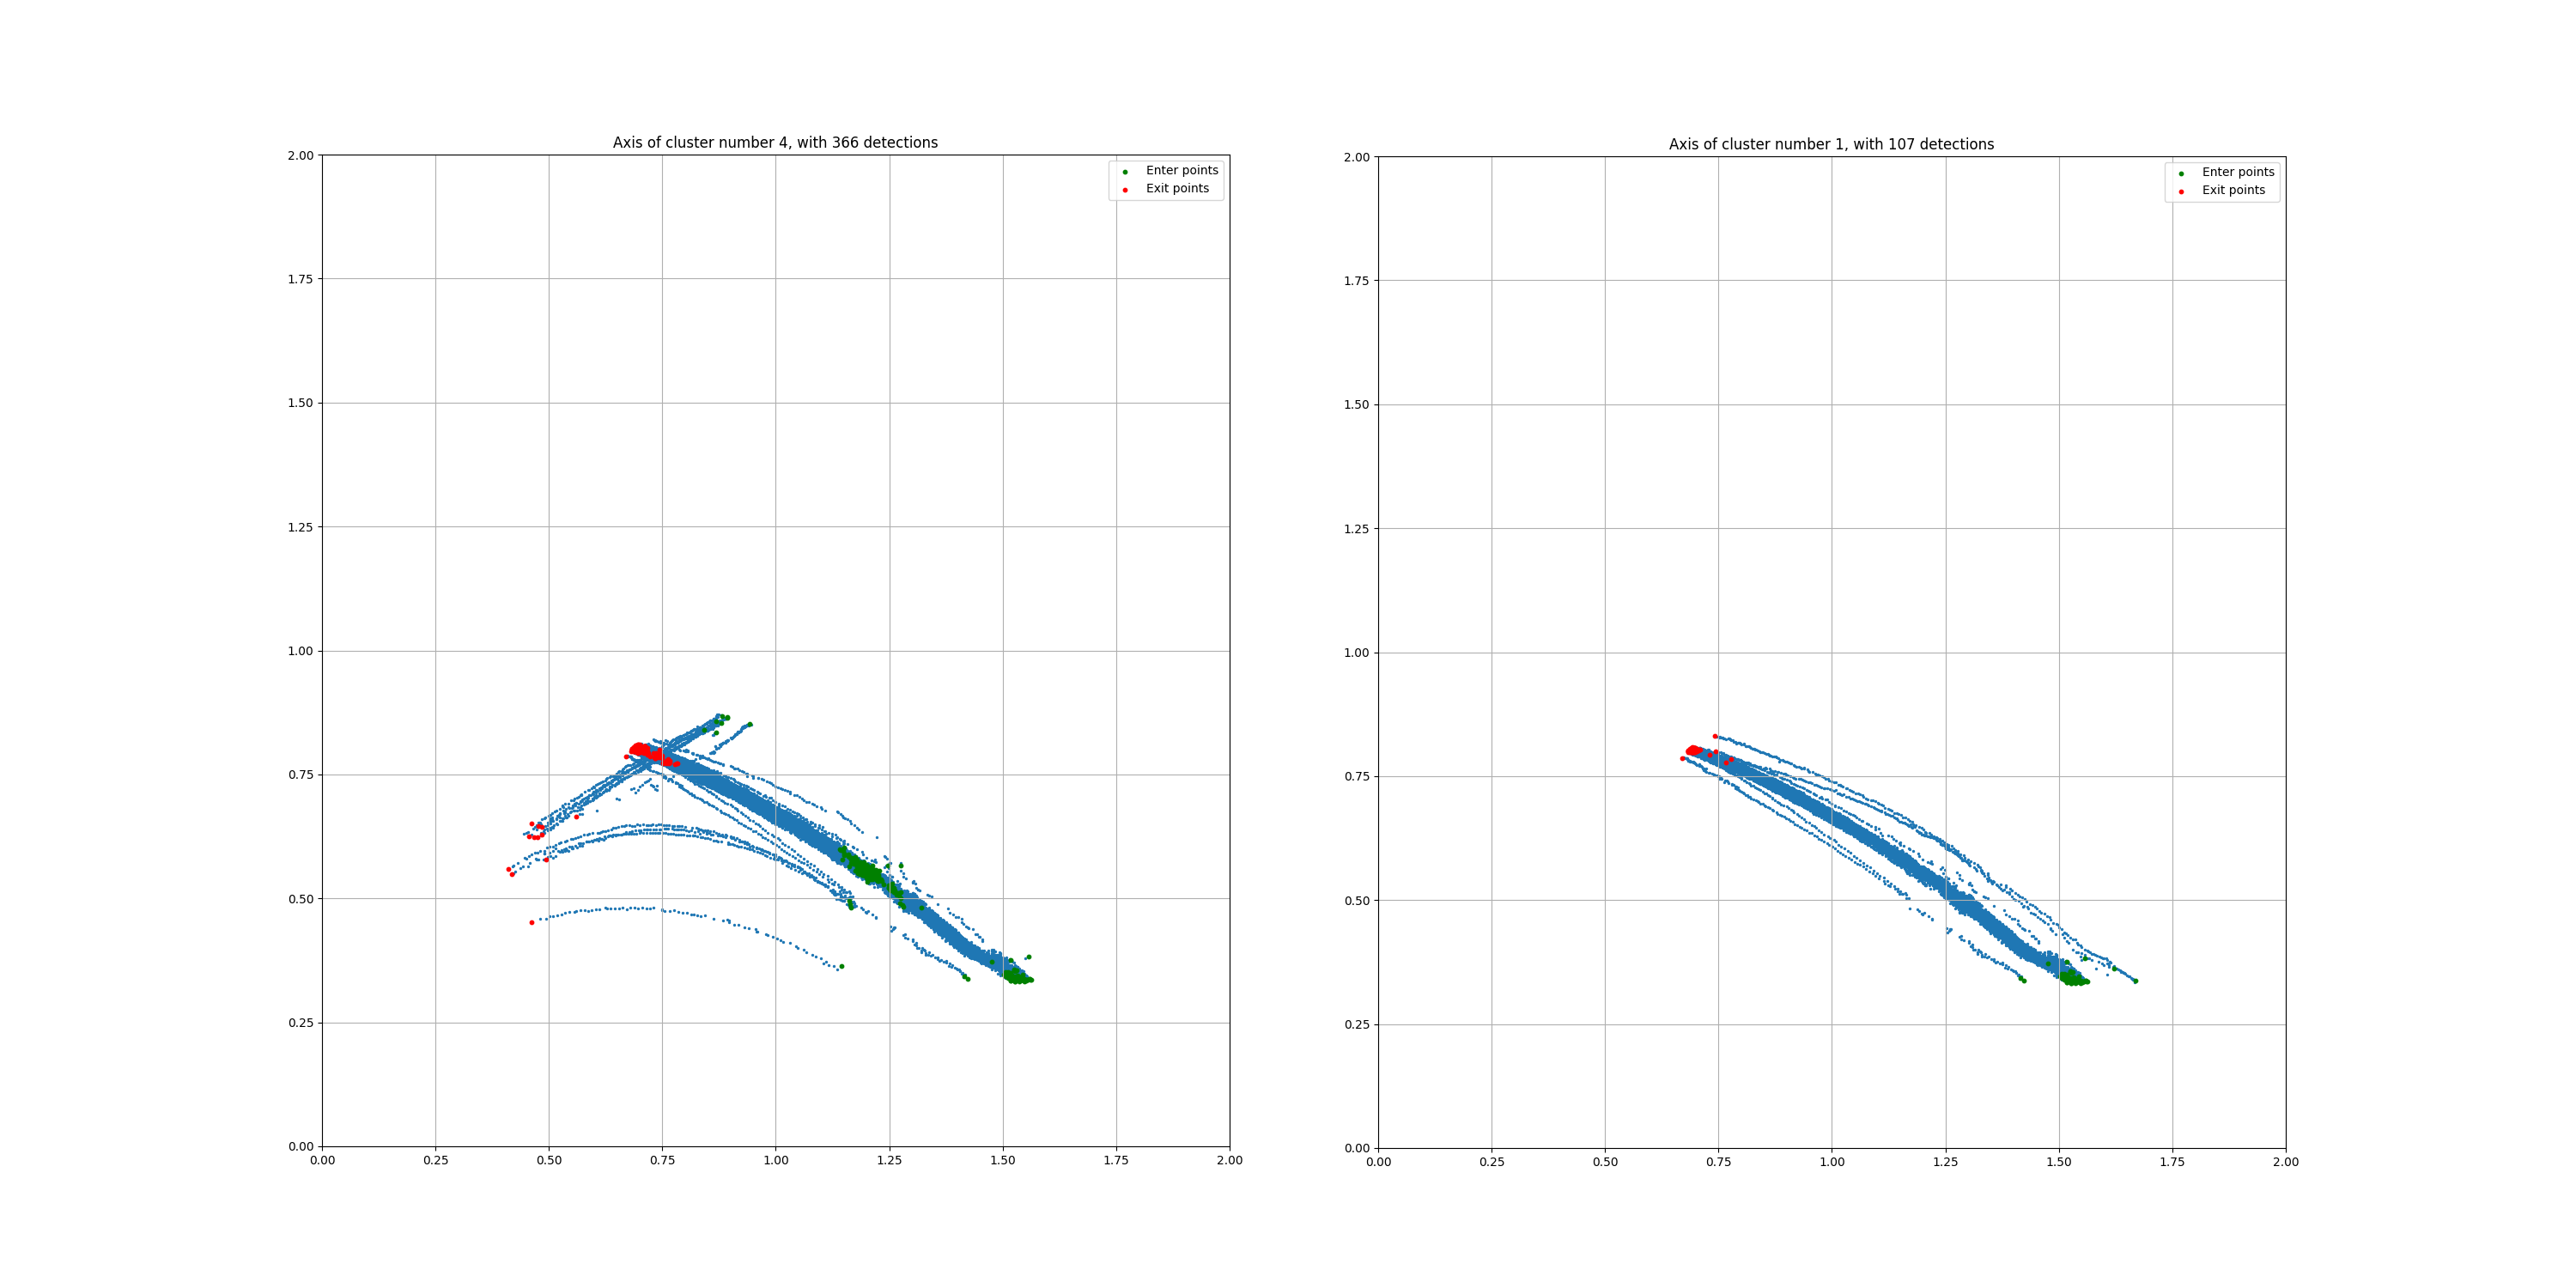
\includegraphics[width=0.65\columnwidth]{bad_clustering/example_kmeans_vs_optics.png}
%     \centering
%     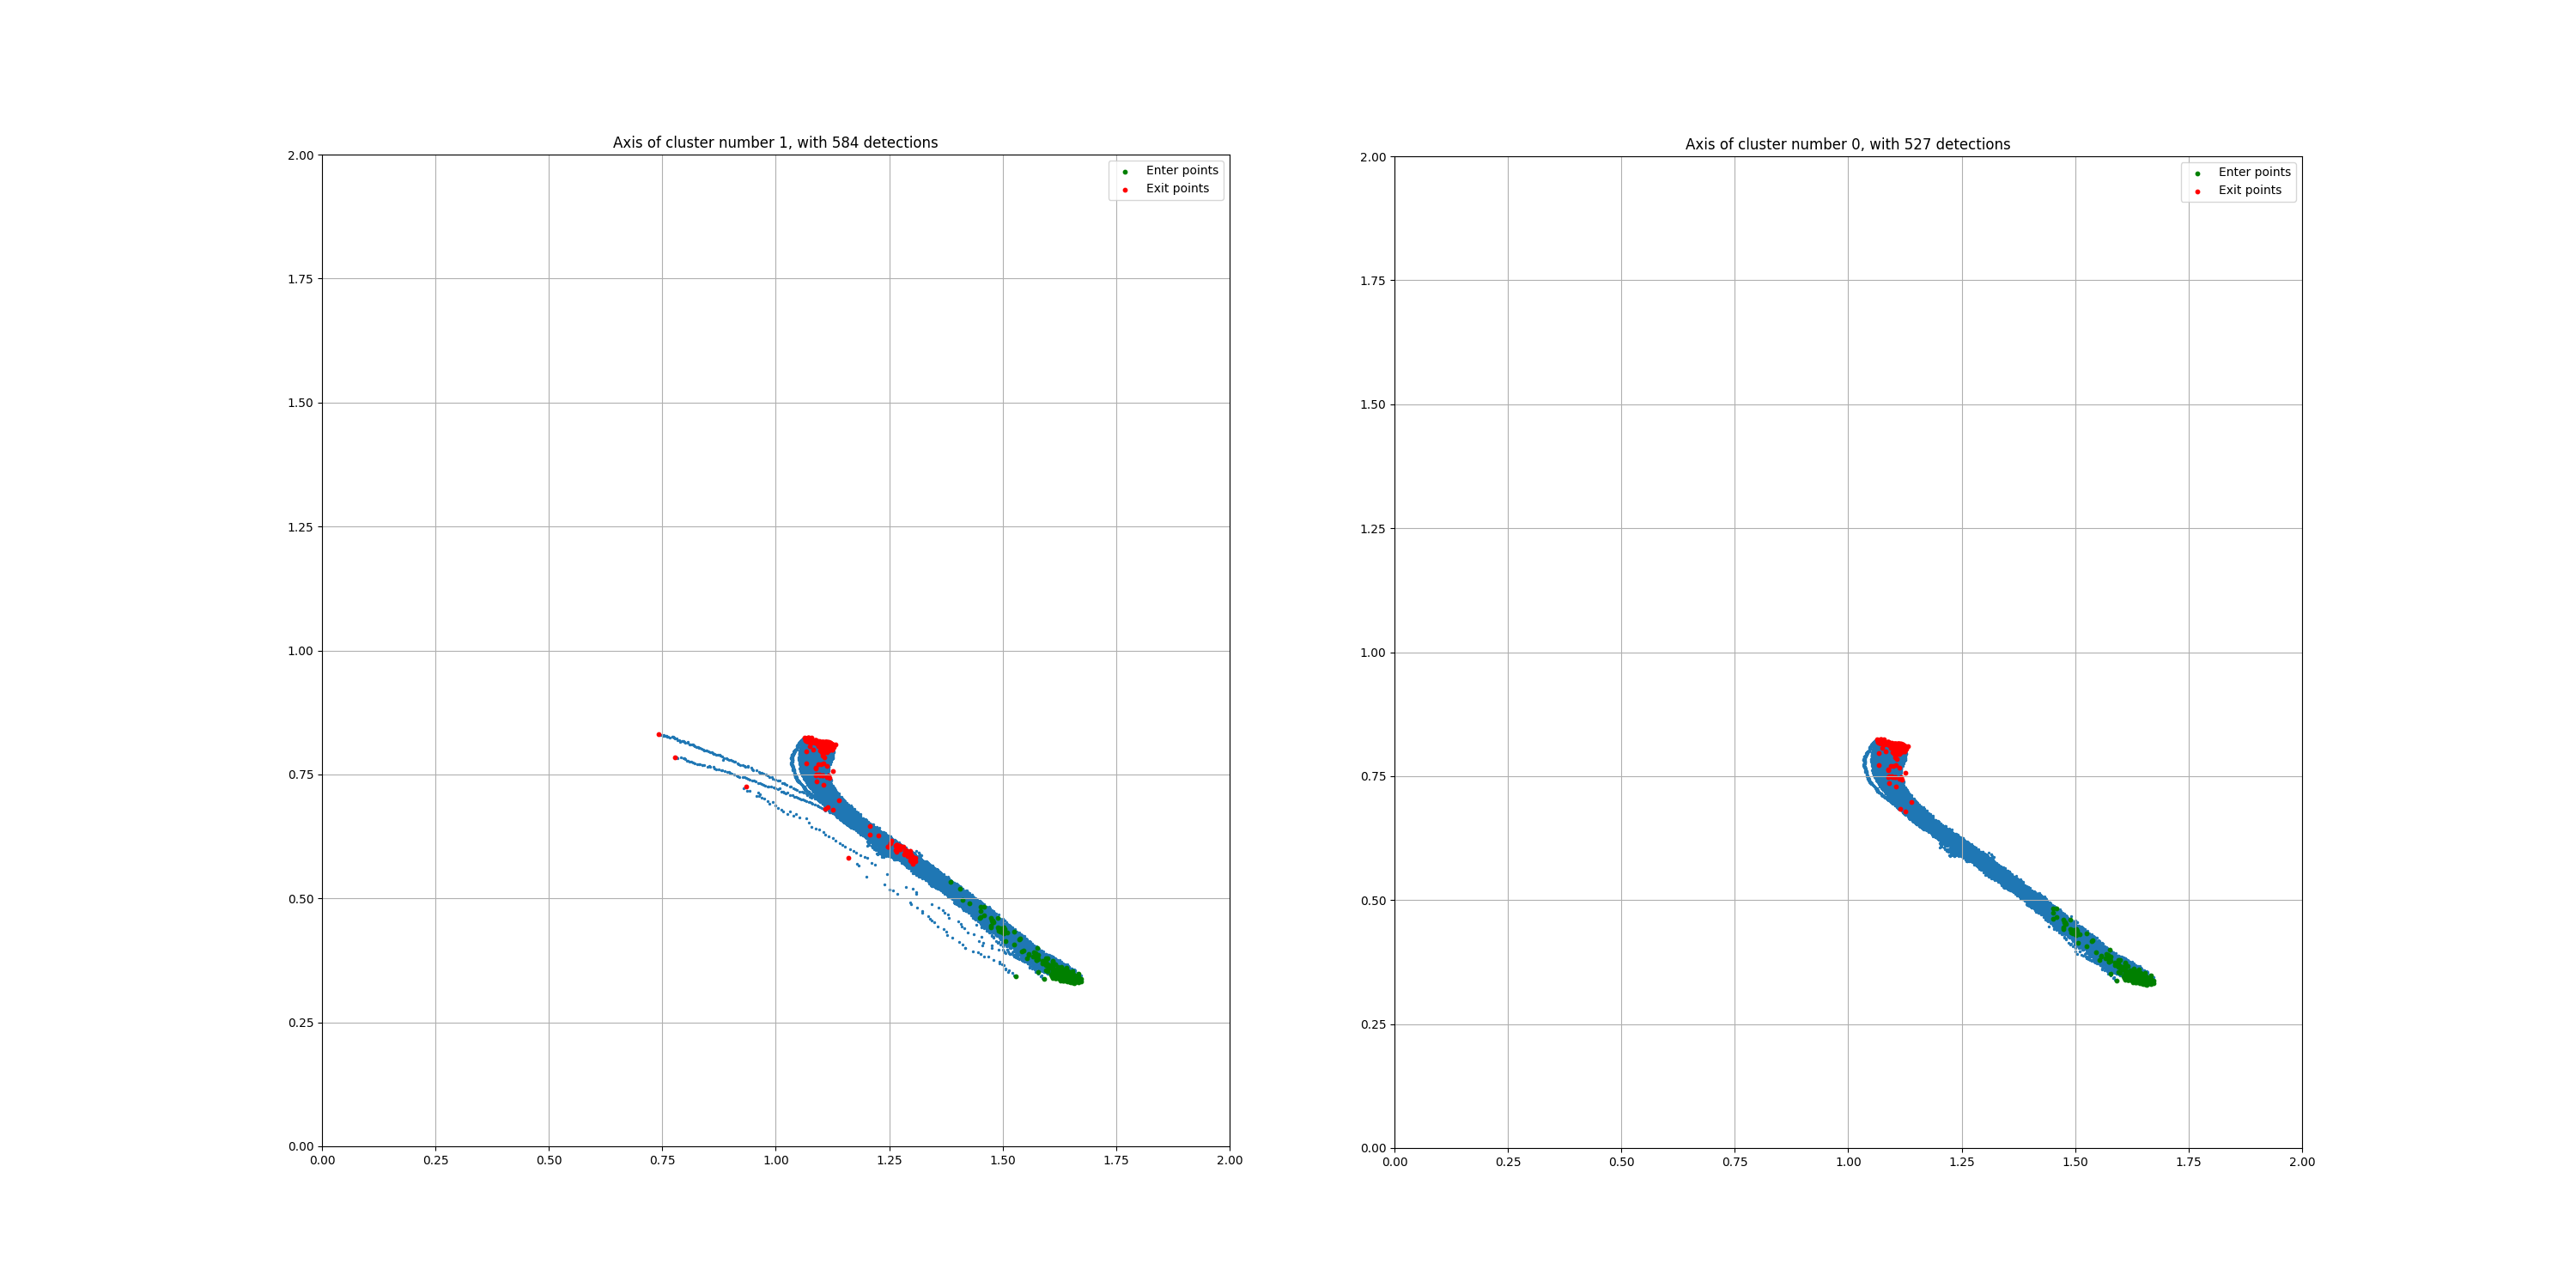
\includegraphics[width=0.65\columnwidth]{bad_clustering/example_birch_vs_optics.png}
%     \centering
%     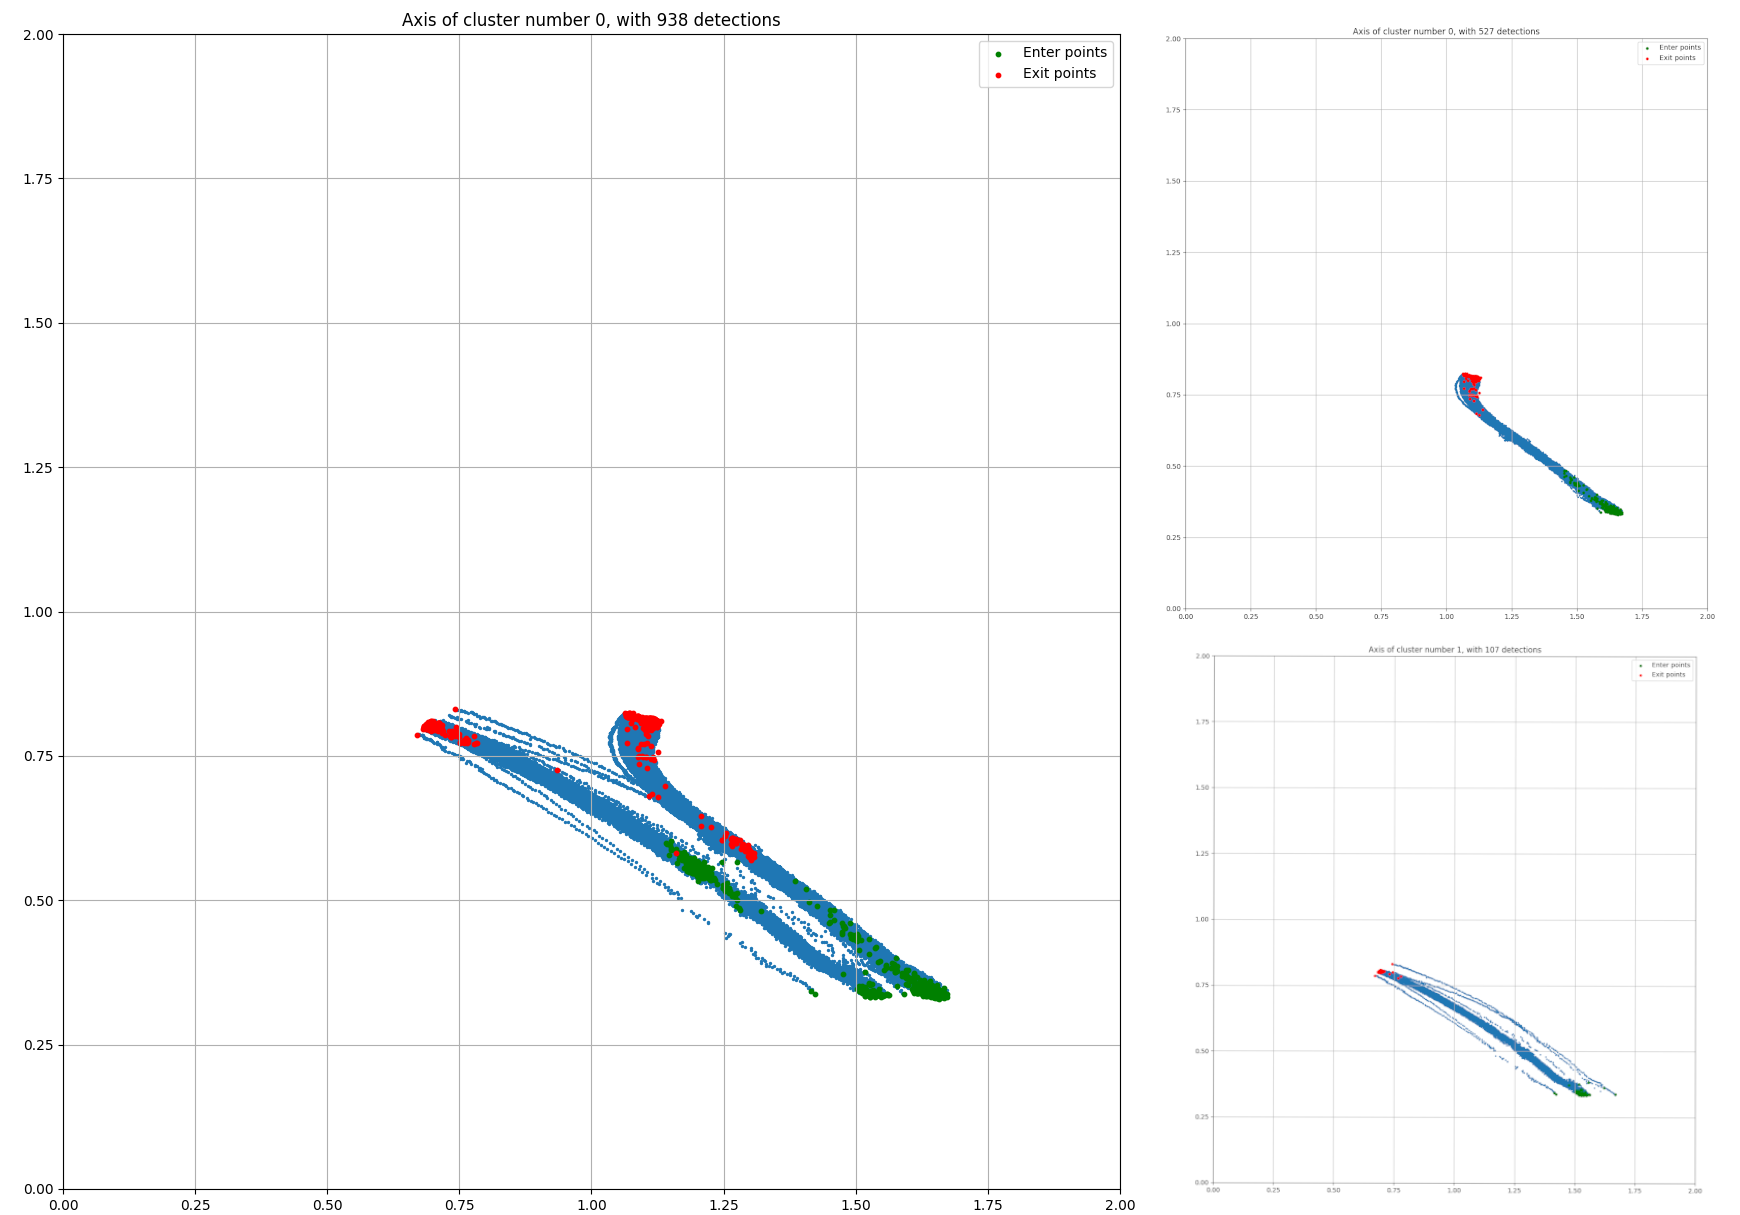
\includegraphics[width=0.65\columnwidth]{bad_clustering/example_dbscan_vs_optics_merged_cluster.png}

%     \caption{KMeans, BIRCH, DBSCAN vs OPTICS}
%     \label{fig: Bad clusters}
% \end{figure}

\paragraph{A BIRCH (Balanced Iterative Reducing and Clustering using Hierarchies)}  egy gyors és hatékony hierarchikus klaszterezési algoritmus, amelyet nagy mennyiségű adat gyors csoportosítására fejlesztettek ki. Az algoritmus célja, hogy az adatokat összesítse a memóriában, és a klaszterek készítése során ne kelljen minden adatpontot az egész adathalmazon végigvinni.
Az algoritmus a következő lépésekből áll:
\begin{enumerate}
    \item Adatok aggregálása: Az adatok aggregálása során az algoritmus egymás mellé helyezi az adatokat az összetartozó klaszterekben. Az aggregálási folyamat során az algoritmus az adatokat kisebb csoportokba osztja, és azokat összevonja egy aggregált reprezentációba.
    \item Hierarchikus csoportosítás: Az algoritmus létrehozza az aggregált adathalmaz hierarchikus reprezentációját. Az adatokat egy fa szerkezetben helyezi el, ahol a gyökér a teljes adathalmaz, a levél pedig az egyes adatpontokat tartalmazza.
    \item Clustering: Az algoritmus elvégzi az adatok klaszterezését a hierarchikus fa struktúra alapján. A klaszterek létrehozása iteratív folyamat, amelyben az algoritmus egymás után dolgozza fel a fa szintjeit. Az algoritmus minden szinten klaszterezést végez, és az előző szinten megtalált klasztereket használja a következő szinten végzett csoportosításhoz.
\end{enumerate}
A BIRCH algoritmus előnye, hogy hatékonyan kezeli a nagy mennyiségű adatokat, és minimális memóriahasználatot igényel. Az algoritmus gyorsan fut, és lehetővé teszi a csoportok hierarchikus struktúrájának vizsgálatát. Azonban az algoritmus nem alkalmas olyan adatokra, amelyeket nehéz aggregálni, és az adatok aggregálása során elveszhetnek a finom részletek.
A futtatott tesztek alapján elmondható, hogy a BIRCH algoritmus sokszor egybevon klaszter bemeneteket vagy kimeneteket, ami miatt több más irányból jövő, vagy több más irányba kilépő objektumokat sorol azonos klaszterekbe.
\begin{math}threshold\end{math} paraméterrel lehet a klaszterek méretét szabályozni, amivel javítható az egybevont klaszterek száma, a kutatás során futtatott tesztek alapján, még így is az OPTICS adta a legtisztább klasztereket.

\paragraph{DBSCAN (Density-Based Spatial Clustering of Applications with Noise)} egy hatékony klaszterezési algoritmus, amely a sűrűség alapján klaszterez. Az algoritmus célja, hogy megtalálja a sűrűségi alapú klasztereket az adathalmazban, és az adatpontokat azonosítsa, amelyek nem tartoznak egyik klaszterhez sem, az úgynevezett zajokat. Az algoritmus három fő paramétere a klaszterek sűrűségének küszöbe $eps$, az adatpontok minimum szomszédjainak száma $min\_samples$ és az adatpontok kiindulási pozíciója.
Az algoritmus lépései a következők:
\begin{enumerate}
    \item Választ véletlenszerűen egy adatpontot, amely még nem lett klaszterezve.
    \item Megtalálja az összes adatpontot, amelyekre az $eps$ sugarú kör középpontjából el lehet jutni.
    \item Ha az adatpontok száma nagyobb, mint a $min\_samples$, akkor létrehoz egy új klasztert és hozzáadja az összes adatpontot a klaszterhez. Ha az adatpontok száma kisebb, mint a $min\_samples$, megjelöli az adatpontot zajként.
    \item Folyamat megismétlése az összes nem klaszterezett adatponttal.
\end{enumerate}

\paragraph{Az OPTICS (Ordering Points To Identify the Clustering Structure)} egy másik klaszterező algoritmus, amely a sűrűség alapú klaszterezést használja. Az algoritmus a DBSCAN-hoz hasonlóan az adatpontok közötti sűrűségi kapcsolatokat használja a klaszterek meghatározásához, de az OPTICS további információt szolgáltat az adathalmaz klaszterezett struktúrájáról. Az algoritmus az adatpontok távolságát és azok sűrűségét is figyelembe veszi a klaszterek meghatározásához.
Az OPTICS algoritmus lépései a következők:
\begin{enumerate}
    \item Válasszunk ki egy véletlenszerű adatpontot, amely még nem került klaszterezésre.
    \item Megkeresi az összes szomszédos adatpontot, és kiszámítja a távolságot az adott adatponttól.
    \item A szomszédos adatpontokat távolság és sűrűség szerint rednezi.
    \item Létrehoz egy ``optikai" sorrendet, amelyben az adatpontokat rendezzük a távolságuk és a sűrűségük szerint. Ez lehetővé teszi, hogy az algoritmus később könnyebben megtalálja a klasztereket és a zajokat.
    \item Ha az adatpontot egy klaszterhez lehet rendelni, akkor adjuk hozzá a klaszterhez.
    \item A folyamatot megismétli az összes nem klaszterezett adatpontra.
\end{enumerate}
Az OPTICS algoritmus előnye, hogy lehetővé teszi a klaszterek és a zajok meghatározását egyaránt, és további információkat is szolgáltat az adathalmaz klaszterezett struktúrájáról, mint például a klaszterek hierarchiájáról és a klaszterek közötti távolságról. Az OPTICS azonban az adathalmazok nagy méretű és magas dimenziós esetében nagyon lassú lehet, és sok erőforrást igényelhet a klaszterezéshez.
Esetünkben azért választottuk az OPTICS-ot a DBSCAN-nel szemben mert az OPTICS még mindig jobban skálázható nagyobb adathalmazokra, és a klaszterek hierarchiáját is meg tudja határozni, ami a későbbi osztályozásnál hasznos lehet.

Paraméterezésben a DBSCAN annyiban különbözik az OPTICS-tól, hogy $max\_eps$ paraméter helyett, ami egy távolság tartományt ad meg, az $eps$ paramétert használja, ami pontos távolságot ad meg.

A \ref{fig:kmeans_cluster}. \ref{fig:optics_cluster}. \ref{fig:birch_cluster}. \ref{fig:optics_cluster_2}. \ref{fig:optics_cluster_3}. képeken, a KMeans, BIRCH klasztereit állítjuk szembe az OPTICS által rendezett klaszterekkel. Látható, hogy az OPTICS, nagyon hatékonyan tudta kiszűrni a zajos trajektóriákat, és nem vont egybe kimeneti vagy bemeneti klasztereket.

\subsection{Paraméterek kiválasztása}
A megfelelő paraméterek kiválasztása a klaszterezéshez igen fonzosnak bizonyult. Ezt a gyűjtött adathalmazokon kézzel kellett finomhangolnunk.
A halmazok minimum számosságát a \begin{math}min\_samples\end{math} paraméterrel lehet szabályozni, a pontok egymástól való távolságának
felső határát \begin{math}max\_eps\end{math}-el lehet megadni. Az távolság kiszámítására használt metódust \begin{math}metric\end{math}-el
lehet megadni. A \begin{math}xi\end{math} paraméterrel az elérési plot minimum meredekségét lehet megadni, ami a klaszterek határát szabja meg.
Az adathalmazra alkalmazható megfelelő paramétereket nem tudtuk generalizálni, kézzel kellett finomhangolnunk. A plotokon látható klaszterek
megtalálásához \begin{math}min\_samples=100\end{math}, \begin{math}max\_eps=0.15\end{math}, \begin{math}metric='minkowski'\end{math} és \begin{math}xi=0.15\end{math}
paramétereket használtunk.

\newpage
\subsection{Közeli klaszterek egyesítése}
Osztályozó algoritmusok tesztelése során azt figyeltük meg, hogy azt is hibának számítottuk amikor az osztályozó algoritmus két nagyon hasonló klaszter közül, amiknek a kimeneti koordinátáik azonosak, csak a bemeneti koordinátáik térnek el, nem a megfelelőbe sorolta az objektumot, viszont ha csak a kimeneti koordináták alapján pontozunk, akkor nem számít hibának. Erre a problémára a kimeneti koordináták alapján való csoportosítás a megoldás (lásd \ref{fig:pooledclusters}).
Az egész klaszterezési eljárást nem kell megismételni, hanem a meglévő klaszterekre alkalmaztunk klaszterezést. Erre a KMeans algoritmust használtuk. Az algoritmus az eredeti és az összevont klaszter középpontok euklideszi távolságának minimalizálásán alapul.
Az algoritmus implementációja pythonban:
\begin{minted}[fontsize=\footnotesize]{python3}
    def kmeans_mse_clustering(
            X: np.ndarray, Y: np.ndarray, 
            n_jobs: int = 10, mse_threshold: float = 0.5
            ) -> Tuple[np.ndarray, KMeans, int, float]:
        Y_exitcluster_centers = calc_cluster_centers(X, Y)
        mse = 9999
        n_clusters = 1
        aoi_labels_best = []
        n_clusters_best = n_clusters
        clr_best = None
        # run min search
        while (mse > mse_threshold):
            clr = KMeans(n_clusters).fit(Y_exitcluster_centers)
            aoi_labels = clr.labels_
            cluster_centers = clr.cluster_centers_
            # calculate mse of original clusters and new pooled clusters
            distance_vector = [euclidean_distance(
                                cluster_centers[l, 0], 
                                Y_exitcluster_centers[i, 0], 
                                cluster_centers[l, 1], 
                                Y_exitcluster_centers[i, 1])
                            for i, l in enumerate(aoi_labels)]
            # if new mse is lower than the previous one, save the new one
            if np.max(distance_vector) < mse:
                mse = np.max(distance_vector)
                n_clusters_best = n_clusters
                clr_best = clr
                aoi_labels_best = aoi_labels
            n_clusters += 1
        Y_reduced_labels = np.zeros(shape=Y.shape, dtype=np.int32)
        for i, l in tqdm.tqdm(enumerate(Y), desc="Reduce labels"):
            Y_reduced_labels[i] = aoi_labels_best[l]
        return (
            Y_reduced_labels, clr_best, n_clusters_best, mse, aoi_labels_best)
\end{minted}
A képeken zölddel jelöltük a bemeneti pontokat és pirossal a kimeneti pontokat. Látható az algoritmus eredménye, a különböző belépési de azonos kilépési pontú útvonalakat egybevonta, ezzel új klasztereket létrehozva.
\begin{figure}[ht]
    \centering
    \begin{subfigure}{0.45\textwidth}
        \centering
        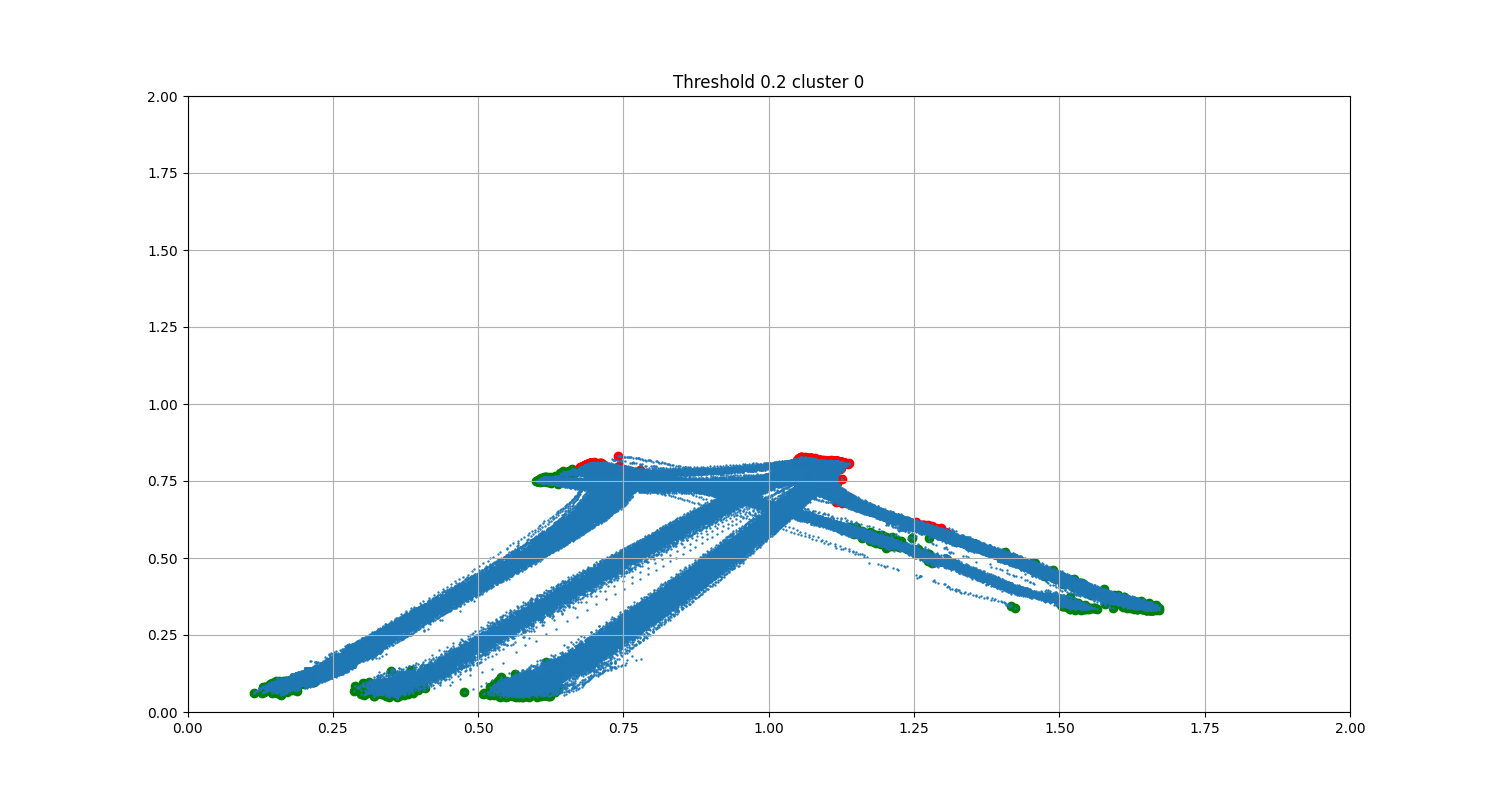
\includegraphics[width=\textwidth]{clustering/KMeansPoolingv2/cluster_0.png}
        \caption{Klaszter 1}
        \label{fig:cluster1}
    \end{subfigure}
    \hfill
    \begin{subfigure}{0.45\textwidth}
        \centering
        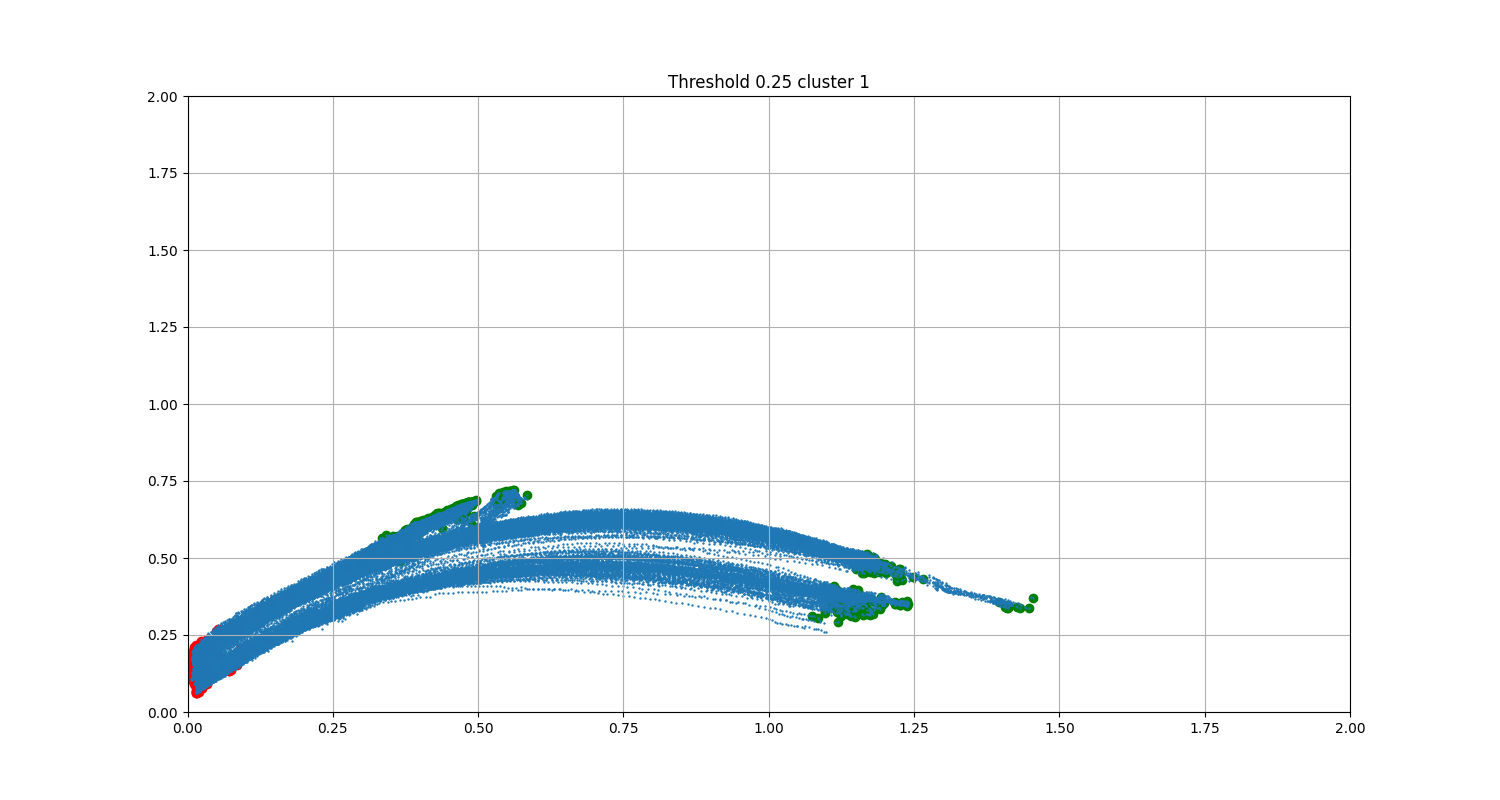
\includegraphics[width=\textwidth]{clustering/KMeansPoolingv2/cluster_1.png}
        \caption{Klaszter 2}
        \label{fig:cluster2}
    \end{subfigure}
    \hfill
    \begin{subfigure}{0.45\textwidth}
        \centering
        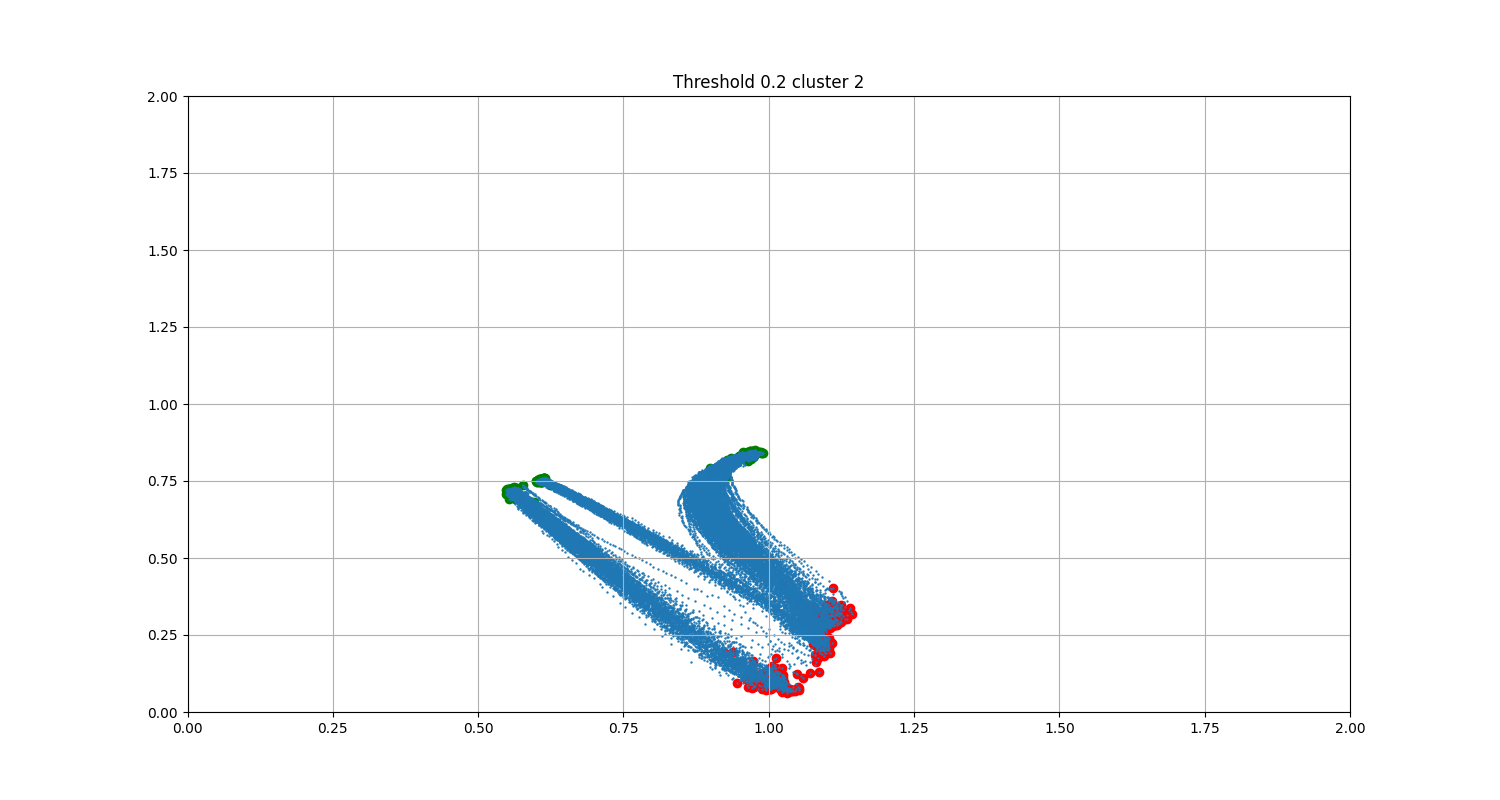
\includegraphics[width=\textwidth]{clustering/KMeansPoolingv2/cluster_2.png}
        \caption{Klaszter 3}
        \label{fig:cluster3}
    \end{subfigure}
    \hfill
    \begin{subfigure}{0.45\textwidth}
        \centering
        \includegraphics[width=\textwidth]{clustering/KMeansPoolingv2/cluster_3.png}
        \caption{Klaszter 4}
        \label{fig:cluster4}
    \end{subfigure}
    \caption{Összevont klaszterek}
    \label{fig:pooledclusters}
\end{figure}

\newpage
\section{Osztályozás}
\subsection{Multiclass}
A több osztályos klasszifikálás egy olyan feladat, amikor több mint 2 osztály van, és minden feature vektor csak egy osztályba tartozhat. Az alapvető megközelítés a többosztályos klasszifikációra az, hogy a modell tanítása során az összes lehetséges kategóriát együttesen kell figyelembe venni. Ez azt jelenti, hogy minden egyes kategóriát egy külön osztályként kell kezelni, és a modell tanulásakor figyelembe kell venni az összes osztályt. Az osztályozó modell célja, hogy az adathalmazból kiválasztott jellemzők és az osztályok közötti kapcsolatok alapján olyan döntési fát vagy osztályozó algoritmust hozzon létre, amely képes az új adatok osztályozására. A multiclass klasszifikációhoz különböző algoritmusok használhatók, például a Random Forest, Support Vector Machine (SVM), k-Nearest Neighbor (kNN), Decision Tree és Deep Neural Network (DNN). A megfelelő algoritmus kiválasztása az adathalmaz méretétől, dimenziójától, a célkitűzésektől és az adatok jellegétől függ.
A Multiclas klasszifikáció kevesebb osztály számnál jó eredeményt adhat, a mi esetünkben 10-15 osztály is lehet, ami azt jelenti, hogy nem lehet elérni nagy pontosságot. Ennyi osztály közül nehéz pontosan eltalálni, melyik osztályba tartozik egy trajektória.
\subsection{Binary}
A binary (kétosztályos) klasszifikáció egy olyan gépi tanulási probléma, amelyben az adathalmazban szereplő objektumokat vagy eseményeket két kategóriába kell osztályozni. Például megkülönböztethetjük a ``spam" és ``nem spam" leveleket, vagy az ``egészséges" és ``beteg" betegeket az orvosi diagnózisban.
Az alapvető megközelítés a binary klasszifikációra az, hogy az osztályozó modell olyan döntési határt hoz létre az adathalmazban található adatok és az osztályok között, amely megkülönbözteti az egyik kategóriába tartozó adatokat a másiktól. Ennek az eredménye egy bináris predikció, amely azt jelzi, hogy egy adott adat az egyik vagy a másik kategóriába tartozik.
\subsection{OneVsRest}
A One-vs-Rest (OvR), más néven One-vs-All (OvA) klasszifikáció egy olyan többosztályos osztályozási technika, amelynek célja, hogy különböző osztályok között megkülönböztetést végezzen. Az OvR-ben a különböző osztályok közötti különbségeket az egyik osztályhoz képest határozzák meg. Ezt az osztályt ``egy" osztálynak nevezik, és a többi osztályt ``a többi" osztályoknak.
Az OvR algoritmusban egy osztályozó modellt hoznak létre minden egyes osztály és a többi osztályok közötti megkülönböztetésre. Ez azt jelenti, hogy ha van például 5 osztályunk, akkor 5 különböző bináris klasszifikátorra van szükségünk, amelyek mindegyike egy adott osztályt különböztet meg a többi osztálytól.
A bináris osztályozók által létrehozott modellt használják az osztályozásra. Az osztályozó modellnek két kimenete van, ``1" vagy ``0". Ha a modell kimenete ``1", akkor az adott minta az adott osztályhoz tartozik, ha a kimenete ``0", akkor az adott minta nem tartozik az osztályhoz.
Az OvR osztályozó előnye, hogy egyszerűen használható, mivel csak bináris osztályozókat kell alkalmazni minden egyes osztályra, és használható, ha az osztályok közötti határok nincsenek jól meghatározva.
\subsection{Machine Learning modellek}
Kutatásunk során több féle machine learning modellt teszteltünk: KNN (KNearesNeighbors), GNB (GaussianNaiveBayes), MLP (MultiLayerPerceptron),
SGD (StochasticGradientDescent), SVM/SVC (SupportVectorMachine/SupportVectorClassifier) \cite{CC01a}, DT (DecisionTree) \cite{Breiman1984ClassificationAR}.
Ezekből a GNB, MLP és SGD nem adott jó eredményeket, ami látható az alábbi táblázatban \ref{table:1}, az eredmények megismétlődtek későbbi tesztekben, ezért
ezeket a modelleket nem tárgyaljuk. A legjobb eredményeket a KNN adta minden esetben 90\% felett teljesített. A második legjobb a DecisionTree lett, ami átlagban
balanced accuracy-ban az SVM felett teljesített, és Top 1 accuracyban is csak tizedekkel maradt le a 7. feature vektor használatakor, az 1. verzióval 4\%-al
jobban teljesített. A mérések eredményei a \ref{table:2}. és \ref{table:3}. táblázatban láthatók.

\begin{table}[H]
    \centering
    \caption{Bellevue Newport V1}
    \label{table:1}
    \begin{tabular}{@{}lccc@{}}
        \toprule
        Metrics            & Balanced & Top 1   & Top 2   \\
        \midrule
        KNN                & 90.57\%  & 95.50\% & 99.12\% \\
        GNB                & 63.92\%  & 73.25\% & 90.10\% \\
        MLP                & 58.49\%  & 81.93\% & 89.43\% \\
        SGD Modified Huber & 45.43\%  & 66.39\% & 83.54\% \\
        SGD Log Loss       & 40.41\%  & 60.70\% & 79.69\% \\
        SVM                & 77.87\%  & 89.29\% & 96.61\% \\
        DT                 & 90.95\%  & 93.64\% & 95.06\% \\
        \bottomrule
    \end{tabular}
\end{table}

\begin{table}[H]
    \begin{minipage}{0.55\textwidth}
        \centering
        \caption{Testset V1}
        \label{table:2}
        \begin{tabular}{@{}lrrr@{}}
            \toprule
            Metrics & Balanced & Top 1   & Top 2   \\
            \midrule
            KNN     & 94.16\%  & 96.71\% & 99.46\% \\
            SVM     & 81.65\%  & 90.82\% & 98.05\% \\
            DT      & 93.11\%  & 94.88\% & 96.03\% \\
            \bottomrule
        \end{tabular}
    \end{minipage}
    \begin{minipage}{0.55\textwidth}
        \centering
        \caption{Cross-Validation V1}
        \label{table:3}
        \begin{tabular}{@{}lrrr@{}}
            \toprule
            Metrics & Balanced & Top 1   & Top 2   \\
            \midrule
            KNN     & 92.60\%  & 96.06\% & 99.38\% \\
            SVM     & 81.21\%  & 89.76\% & 97.79\% \\
            DT      & 92.43\%  & 94.55\% & 95.97\% \\
            \bottomrule
        \end{tabular}
    \end{minipage}
\end{table}

\begin{table}[H]
    \begin{minipage}{0.55\textwidth}
        \centering
        \caption{Testset V7 Stride 15}
        \label{table:4}
        \begin{tabular}{@{}lrrr@{}}
            \toprule
            Metrics & Balanced & Top 1   & Top 2   \\
            \midrule
            KNN     & 92.08\%  & 95.61\% & 98.66\% \\
            SVM     & 88.72\%  & 93.86\% & 98.92\% \\
            DT      & 89.46\%  & 93.30\% & 94.55\% \\
            \bottomrule
        \end{tabular}
    \end{minipage}
    \begin{minipage}{0.55\textwidth}
        \centering
        \caption{Testset V7 Stride 30}
        \label{table:5}
        \begin{tabular}{@{}lrrr@{}}
            \toprule
            Metrics & Balanced & Top 1   & Top 2   \\
            \midrule
            KNN     & 92.68\%  & 95.96\% & 98.79\% \\
            SVM     & 88.67\%  & 93.49\% & 98.91\% \\
            DT      & 89.87\%  & 93.17\% & 94.53\% \\
            \bottomrule
        \end{tabular}
    \end{minipage}
\end{table}

% \begin{table}[]
%     \centering
%     \begin{tabular}{|lccc|}
%         \hline
%         \multicolumn{4}{|c|}{\begin{tabular}[c]{@{}c@{}}Cross-Validation Average Accuracy\\ Feature Vector v1\end{tabular}} \\ \hline
%         \hline
%         \multicolumn{1}{|l|}{Metrics} & \multicolumn{1}{c|}{Balanced} & \multicolumn{1}{c|}{Top 1}   & Top 2                \\ \hline
%         \multicolumn{1}{|l|}{KNN}     & \multicolumn{1}{c|}{92.60\%}  & \multicolumn{1}{c|}{96.06\%} & 99.38\%              \\ \hline
%         \multicolumn{1}{|l|}{SVM}     & \multicolumn{1}{c|}{81.21\%}  & \multicolumn{1}{c|}{89.76\%} & 97.79\%              \\ \hline
%         \multicolumn{1}{|l|}{DT}      & \multicolumn{1}{c|}{92.43\%}  & \multicolumn{1}{c|}{94.55\%} & 95.97\%              \\ \hline
%     \end{tabular}
%     \caption{Cross-Validation Feature Vector V1}
%     \label{table:5}
% \end{table}

\begin{table}[H]
    \begin{minipage}{0.55\textwidth}
        \centering
        \caption{Cross-Validation V7 Stride 15}
        \label{table:6}
        \begin{tabular}{@{}lrrr@{}}
            \toprule
            Metrics & Balanced & Top 1   & Top 2   \\
            \midrule
            KNN     & 90.74\%  & 95.49\% & 98.39\% \\
            SVM     & 87.36\%  & 94.03\% & 98.85\% \\
            DT      & 89.12\%  & 93.56\% & 94.95\% \\
            \bottomrule
        \end{tabular}
    \end{minipage}
    \begin{minipage}{0.55\textwidth}
        \centering
        \caption{Cross-Validation V7 Stride 30}
        \label{table:7}
        \begin{tabular}{@{}lrrr@{}}
            \toprule
            Metrics & Balanced & Top 1   & Top 2   \\
            \midrule
            KNN     & 91.15\%  & 95.64\% & 98.54\% \\
            SVM     & 87.28\%  & 93.69\% & 98.60\% \\
            DT      & 89.55\%  & 93.73\% & 95.15\% \\
            \bottomrule
        \end{tabular}
    \end{minipage}
\end{table}

\begin{table}[ht]
    \centering
    \caption{Clusters (OPTICS)}
    \label{tab:clusters-optics}
    \begin{tabular}{@{}lrrrr@{}}
        \toprule
            & \multicolumn{1}{l}{Top-1} & \multicolumn{1}{l}{Top-2} & \multicolumn{1}{l}{Top-3} & \multicolumn{1}{l}{Balanced Accuracy} \\ \midrule
        KNN & 95.69\%                   & 99.01\%                   & 99.76\%                   & 92.14\%                               \\
        SVM & 86.45\%                   & 96.52\%                   & 98.94\%                   & 76.57\%                               \\
        DT  & 95.61\%                   & 97.05\%                   & 97.40\%                   & 92.68\%                               \\ \bottomrule
    \end{tabular}
\end{table}
\begin{table}[ht]
    \centering
    \caption{Pooled clusters (K-Means MSE Search)}
    \label{tab:pooled-clusters}
    \begin{tabular}{@{}lrrrr@{}}
        \toprule
            & \multicolumn{1}{l}{Top-1} & \multicolumn{1}{l}{Top-2} & \multicolumn{1}{l}{Top-3} & \multicolumn{1}{l}{Balanced Accuracy} \\ \midrule
        KNN & 98.74\%                   & 99.79\%                   & 99.79\%                   & 98.73\%                               \\
        SVM & 92.93\%                   & 98.83\%                   & 99.93\%                   & 93.14\%                               \\
        DT  & 96.92\%                   & 97.32\%                   & 97.32\%                   & 97.03\%                               \\ \bottomrule
    \end{tabular}
\end{table}


\paragraph{KMeans csoportösszevonás} Az általunk létrehozott csoportösszevonó algoritmus azért volt szükséges, mert a fentebb megjelenített pontosság értékek megtéveszthetők lehetnek. Mivel az útvonalak bemeneti és kimeneti pontok alapján vannak elsősorban csoportosítva, így az a predikció is hibának számít ami az eredeti csoporthoz közeli csoportba sorolta a járművet. Ezt nem feltétlenül kell hibának néznünk, mert nekünk a kimeneti pontot kell figyelembe vennünk, ami lehet ugyan az két csoportnál, amiknek különböző a bemeneti pontjuk (lásd \ref{fig:pooledclusters}). Az összevonás előtti és utáni eredmények megtekinthetők a \ref{tab:clusters-optics} és \ref{tab:pooled-clusters} táblázatokban, amik a Bellevue NE adathalmazon futtatott kiértékelésből származnak. Az eredmények alapján látható, hogy a csoportösszevonás javította a predikciókat, a Top-1 és Top-2 pontosságok nőttek, a Balanced Accuracy pedig 5-10\%-al javult a KNN és SVM esetében.


\paragraph{A K-Nearest Neighbors (KNN)} egy egyszerű és hatékony osztályozó algoritmus, amely az adatok közötti távolság alapján osztályozza a bemeneti adatokat. Az algoritmus lényege, hogy egy adott bemeneti adathoz hasonló adatokat keres a tanuló adathalmazból, majd azok osztálycímkéit megnézve meghatározza az adat osztályát.
Az algoritmus először szükséges, hogy az adatokat előkészítse. Ez magában foglalhatja az adatok normalizálását, standardizálását, az outlier-ek kezelését, valamint a kategorikus adatok konvertálását numerikus formába.
Az algoritmus működése a következő lépésekből áll:
\begin{enumerate}
    \item Távolságok számítása: Az algoritmus először számítja ki az összes tanuló adatpont és a bemeneti adatpont közötti távolságot. A leggyakrabban használt távolságmértékek az euklideszi és manhattani távolságok.
    \item K legközelebbi szomszéd kiválasztása: Az algoritmus a távolságok alapján kiválasztja a K legközelebbi szomszédot a bemeneti adatpontnak. A K értéke általában egy páros szám, hogy elkerüljük a döntések holtversenyét.
    \item Döntés meghozása: Az algoritmus a K legközelebbi szomszéd osztálycímkéinek többségi szavazatával dönti el, hogy melyik osztályba sorolja a bemeneti adatpontot.
\end{enumerate}
Az előnye, hogy a KNN algoritmus könnyen értelmezhető és egyszerűen használható. Az algoritmus jól működik a kisebb méretű adathalmazokon, különösen akkor, ha az adatok egyszerű struktúrával rendelkeznek. A KNN továbbá jól alkalmazható olyan feladatokra, ahol a határok nem lineárisak, és ahol a szokásos statisztikai módszerek nem elegendőek. Az algoritmusnak azonban vannak korlátai, például az, hogy az algoritmus futási ideje növekszik az adathalmaz méretével, valamint hogy az eredmények érzékenyek lehetnek az adatpontok elhelyezkedésére.

\paragraph{Az SVM (Support Vector Machine)} egy erőteljes, nemlineáris osztályozó algoritmus, amelynek célja egy határvonal (vagy hipersík) megtalálása az adatok között. Az algoritmus a bemeneti adatokat olyan módon osztályozza, hogy a döntési határvonal az osztályok közötti legnagyobb távolságot biztosítsa. Ez a távolság a két legközelebbi adatpont közötti távolság, és margin-nek nevezik.
Az SVM algoritmus működése a következő lépésekből áll:
\begin{enumerate}
    \item Adatok előkészítése: Az adatokat előkészítjük, eltávolítjuk a hiányzó adatokat, valamint normalizáljuk vagy standardizáljuk az adatokat a hatékonyabb tanulási folyamat érdekében.
    \item Határvonal (hipersík) keresése: Az SVM algoritmus az adatokat olyan módon osztályozza, hogy a határvonal a két osztály közötti legnagyobb távolságot biztosítsa. Az algoritmus megtalálja az optimális hipersíkot, amely a legnagyobb margin-t biztosítja, amely egyenlő a két legközelebbi adatpont távolságával.
    \item Osztályozás: Az algoritmus az új adatokat a hipersíkon való pozíciójuk alapján osztályozza. Az algoritmus eldönti, hogy az új adat melyik oldalon található a határvonalon.
\end{enumerate}
Az SVM előnye, hogy jól működik a magas dimenziós adatokon és olyan feladatokon, ahol az osztályok közötti határok nem lineárisak. Az SVM továbbá rendkívül hatékony az outlier-ek kezelésében, mivel csak azok a pontok határozzák meg a határvonalat, amelyek a legközelebb vannak hozzá. Az SVM azonban egy nehézkes algoritmus, amelynek tanítása hosszabb ideig tart, ha nagy adathalmazokat kell kezelni. Az algoritmus hiperparamétereinek finomhangolása továbbá kihívást jelenthet, különösen ha nem rendelkezünk megfelelő előzetes tudással az adathalmazról.
\paragraph{SVM Paraméterek} Több féle ``kernel function" - szűrő - közül választhatunk, ami lehet lineáris, polinomiális, exponenciális stb. Mi az RBF (Radial Basis Function) exponenciális szűrőt használtuk, aminek két fő paramétere van: $C$ és $\gamma$. $C$ az SVM egy általános paramétere, ami másik szűrők használatakor is jelen van. Ez a paraméter határozza meg mennyire legyen elsimítva az osztályok közötti határ. Alacsony $C$ sima határvonalhoz vezet, amíg a magas $C$ azt okozza, hogy minden tanító adatot pontosan osztályozni tudjon. A $\gamma$ prarméter, azt határozza meg, hogy egy tanító adatnak mekkora befolyása van. Magas $\gamma$ esetén az egymáshoz közelebbi adatok magas befolyással bírnak egymásra. Méréseink során azt tapasztaltuk, hogy az SVM tényleg gyors és hatékony, még nagy tanító halmaz mellett is.

\paragraph{A Decision Tree (döntési fa)} egy olyan algoritmus, amely a bemeneti adatok alapján egy hierarchikus fastruktúrát hoz létre. Az ilyen fastruktúra minden csomópontjában egy adatfajta tulajdonsága áll, és a levélcsomópontokban pedig a végleges osztálycímkék találhatók. A döntési fában minden ág egy adott tulajdonság értékét reprezentálja, és a fa felépítése során az algoritmus igyekszik minél jobban felosztani a bemeneti adatokat az osztályok között.
A Decision Tree osztályozó algoritmus létrehozása során a következő lépések szükségesek:
\begin{enumerate}
    \item Adatok előkészítése: Az adatokat elő kell készíteni az osztályozó algoritmus számára, amely magában foglalhatja az adatok előfeldolgozását, a hiányzó értékek kezelését és a kategórikus változók átalakítását számszerű adatokká.
    \item Fa építése: A faépítés során az algoritmus megpróbálja kiválasztani a legmegfelelőbb tulajdonságot a bemeneti adatok osztályozásához, majd a tulajdonság értékeitől függően felosztja az adatokat az algoritmus által meghatározott csoportokba. Az algoritmus folytatja ezt a folyamatot minden ágba, amíg el nem éri a megállási feltételt.
    \item Fa értékelése: Az értékelés során az algoritmus osztálycímkéket rendel a bemeneti adatokhoz a fa segítségével.
\end{enumerate}
A döntési fa osztályozó algoritmus előnye, hogy a modell könnyen értelmezhető és átlátható, így könnyen megérthető, hogy a modell hogyan dönt a különböző osztálycímkékkel kapcsolatban. Az algoritmus továbbá jól alkalmazható kategórikus és numerikus változók kezelésére, valamint skálázható és gyorsan futtatható nagyobb adathalmazokon is.
Egy döntési fát könnyű vizualizálni és kirajzolni, hisz egyszerű ``if-else" logikai elágazásokból épül fel (lásd \ref{DTVis}). Nagy és komplex fák alakulhatnak ki, amik túltanulást eredményezhetnek, és már kis eltérések a tanító halmazban nagy eltéréseket eredményezhetnek a fa logikájában.

\begin{figure}[htbp]
    \centering
    \includegraphics[width=1\columnwidth]{DT_7x0.5_decision_tree_2.gv.pdf}
    \caption{DecisionTree Gráf Vizualizáció}
    \label{DTVis}
\end{figure}

\subsection{Feature vektorok}
Ahogyan klaszterezésnél is, fontos meghatározni egy olyan feature vektort, ami a legjobban jellemzi a trajektóriát. Ebben a papírban
két fajta vektor verziót fogunk tárgyalni, amik a tesztek során a legjobban teljesítettek. Az egyik a legelső verzió amit kipróbáltunk,
a másik a hetedik verzió, ami jobban teljesített, mint az összes többi 2-6 verzió.
\paragraph{Az első verzió} Felépítése a következő \begin{math}[x_0, y_0, v_{x_0}, v_{y_0}, x_m, y_m, x_l, y_l, v_{x_l}, v_{y_l}]\end{math}, ahol \begin{math}m\end{math}
index jelöli az időben középen elhelyezkedő detektálást, az \begin{math}l\end{math} index pedig az utolsó, legfrissebb detektálást jelőli.
Ez a vektor jól reprezentálja a valós idejű futás közben keletkező trajektóriákat, mert egyszerre több száz detektálást objektumonként
nem lehet eltárolni a memórában, hanem egy meghatározott méretű buffert kell alkalmazni, aminek mi 15 vagy 30 detektálást adtunk.
Az adathalmazban eltárolt trajektóriák ennél a buffernél több detektálást tartalmaznak, ezért az első verziónál a trajektóriát \begin{math}k\end{math}
részre osztottuk, így egy trajektória szelet mérete \begin{math}s_n = n_d/k\end{math}, ahol \begin{math}n_d\end{math} a detektálások számossága
a trajektóriában. Ezekből a szeletekből képeztük az egyes feature vektorokat.
\paragraph{A hetedik verzió} Felépítése \begin{math}[x_0 \cdot w_1, y_0 \cdot w_2, v_{x_0} \cdot w_3, v_{y_0} \cdot w_4, x_l \cdot w_5, y_l \cdot w_6, v_{x_l} \cdot w_7, v_{y_l} \cdot w_8]\end{math}.
Ennél a verziónál használtunk súlyokat, ahol \begin{math}w_1=1\end{math}, \begin{math}w_2=1\end{math}, \begin{math}w_3=100\end{math}, \begin{math}w_4=100\end{math},
\begin{math}w_5=2\end{math}, \begin{math}w_6=2\end{math}, \begin{math}w_7=200\end{math}, \begin{math}w_8=200\end{math}. Mivel a sebességek két
nagyságrenddel kisebbek mint a koordináták, ezért felszoroztuk őket 100-as súlyokkal. Hogy a 15-30 detektálás nagyságú bufferekben nagyobb hangsúlyt kapjanak a legfrissebb
koordináták és sebességek, így azok 2-es és 200-as szorzót kaptak. A mérések ereményéből azt lehet levonni, hogy a 30-as bufferméret használata nem kifizetődő, hiszen nem növekedett a pontosság, és kétszer akkora memória igénye van.
\paragraph{Teszt eredmények} Azt mutatják, hogy az utóbbi verzió növelte az SVM pontosságát, viszont rontott a KNN és DT pontosságán (lásd \ref{table:5}). Még nagyobb adathalmazok esetén, ahol pár ezer trajektória helyett több tíz vagy akár százezer van, érdemes megfontolni, hogy a 7. verzióval tanítunk be SVM modellt, mivel a KNN futási ideje ekkora adatmennyiség esetén sokkal lassabb lesz.

\subsubsection{Adatdúsítás}
Hogy minél pontosabban reprezentáljuk a valód idejű futást és növeljük a tanító adathalmazt, egy trajektóriából több feature vektort állítunk elő.
Ezeknek a számosságát, a feature vektorokat generáló algoritmusban szabtuk meg. Ezzel azt is szabályoztuk, hogy mekkora időszeletből prediktáljon
a modellünk. Mint ahogy fent is említettük, valós időben 15, max 30 detektálást érdemes tárolni a bufferben. A mérési eredmények azt mutatják, hogy
15 és a 30 nagyságú buffer közt nincs nagy különbség pontosságban. Futási idő szempontjából érdemes lehet a 15 nagyságú buffert választani,
ha van elég tanító adat, és időt akarunk spórolni tanításnál, akkor a 30 nagyságú buffert is választhatjuk, mivel így felére csökken a feature vektorok száma, ez kevesebb tanítási időt jelent, viszont futás közben lesz nagyobb a memóriaigény.
%\subsubsection{Klassz kiegyenlítés}
\subsection{Pontosság mérése}
A pontosság mérésére háromféle metrikát használtunk.
\paragraph{Accuracy Score}
Ha \begin{math}\hat{y_i}\end{math} az \begin{math}i\end{math}. minta predikciója és \begin{math}y_i\end{math} a hozzátartozó valódi érték,
akkor az eltalált predikciók és összes predikció hányadosa, amit így lehet leírni:\break
\begin{equation}
    \texttt{accuracy}(y, \hat{y}) = \frac{1}{n_\text{samples}} \sum_{i=0}^{n_\text{samples}-1} 1(\hat{y}_i = y_i)
\end{equation}
\paragraph{Balanced Accuracy}
amit azért használtunk, hogy az adathalmaz kiegyensúlyozatlansága miatt ne kapjunk fals pontosságot. Ha minden osztályra egyenlően jól teljesít a klasszifikációs modellünk, akkor a sima \emph{Accuracy}-t kapjuk vissza.
Ha a teszt adathalmaz kiegyensúlyozatlansága miatt az egyik osztálynak jobb a pontossága, mint egy másiknak, akkor ezt az értéket elosztja a számával. Ha az \begin{math}y_i\end{math} a valódi értéke az \begin{math}i\end{math}. mintának, és \begin{math}w_i\end{math} a hozzátartozó súly, akkor ezt a súlyt a következőképpen korrigáljuk:
\begin{equation}
    \hat{w}_i = \frac{w_i}{\sum_j{1(y_j = y_i) w_j}}
\end{equation}
ahol \begin{math}1(x)\end{math} a karakterisztikus függvény. Adott a \begin{math}\hat{y_i}\end{math} perdikció az \begin{math}i\end{math}.
mintának, így a balanced accuracy-t így definiálhatjuk:
\begin{equation}
    \texttt{balanced-accuracy}(y, \hat{y}, w) = \frac{1}{\sum{\hat{w}_i}} \sum_i 1(\hat{y}_i = y_i) \hat{w}_i
\end{equation}
\paragraph{Top-K Accuracy}
az \emph{Accuracy Score} egy generalizált változa-ta. A különbség az, hogy a predikció akkor számít igaznak, ha beletartozik a \begin{math}k\end{math}
legmagasabb valószínűségű predikciók közé. Ha \begin{math}\hat{f}_{i,j}\end{math} a \begin{math}i\end{math}. mintának a \begin{math}j\end{math}. legmagasabb
predikciója, és \begin{math}y_i\end{math} a hozzátartozó valódi predikció, akkor az eltalált predikciók és az összes minta hányadosát így
lehet definiálni:
\begin{equation}
    \texttt{top-k accuracy}(y, \hat{f}) = \frac{1}{n_\text{samples}} \sum_{i=0}^{n_\text{samples}-1} \sum_{j=1}^{k} 1(\hat{f}_{i,j} = y_i)
\end{equation}
ahol \begin{math}k\end{math} a megengedett találgatások száma, és \begin{math}1(x)\end{math} a karakterisztikus függvény.
\subsubsection{Adathalmaz szétválasztás}
Egy predikciós függvény paramétereit finomhangolni egy adathalmazon, majd tesztelni ugyan azon a halmazon nem jó módszer.
Ez tökéletes pontosságot eredményezne, de a valóságban, még nem láttot adatokon nem lenne használható. Ezt a hibát túltanításnak - \textit{Overfitting} - hívják.
Hogy elkerüljük ezt, egy megszokott módszer felügyelt gépi tanulásnál, egy teszt adathalmaz félrerakása amin csak leteszteljük a végső model pontosságát.
A folyamatot szemléltető ábrán \ref{fig:TrainTestSplit} látható a paraméterek finomhangolása és a tesztelés folyamata.

\begin{figure}[H]
    \centering
    \includegraphics[width=.65\columnwidth]{grid_search_workflow.png}
    \centering
    \caption{Tanítási folyamat. \href{https://scikit-learn.org/stable/_images/grid_search_workflow.png}{Forrás}}
    \label{fig:TrainTestSplit}
\end{figure}

\subsubsection{Cross Validation - Kereszt validáció}
A fennti problémára megoldás lehet, hogy 3 részre osztjuk az adathalmazt. Egy tanító, egy validációs és egy teszt adathalmazra.
A tanító adathalmazon tanítjuk be a modellt, a validációs adathalmazon pedig finomhangoljuk a paramétereket, és a teszt adathalmazon teszteljük a modell pontosságát.
Ez sok esetben az adathalmaz méretének a harmadára csökkenti a tanító adathalmazt, ami nem kívánatos. Ezt a problémát oldja meg a kereszt validáció \ref{fig:KFold}.

\begin{figure}
    \centering
    \includegraphics[width=.65\columnwidth]{grid_search_cross_validation.png}
    \caption{KFold cross-validation. \href{https://scikit-learn.org/stable/_images/grid_search_cross_validation.png}{Forrás}}
    \label{fig:KFold}
\end{figure}

\paragraph{KFold} Egy olyan cross-validation metódus, ahol a tanító adathalmazt
$k$ részre osztják, ebből a $k$ részből egyet kiválasztanak validációra, így keletkezik egy tanító és validáló adathalmaz. A tanító adathalmazon betanítanak
egy modellt, aminek a pontosságát megmérik a validáló adathalmazon. Ezt az algoritmust $k$-szor ismétlik meg, úgy hogy minden rész egyszer legyen validáló
adathalmaz. Ezeknek a méréseknek az átlag pontosságát szokták kiszámolni, és az eredmények alapján finomhangolni a model paramétereit. A cross-validációból származó eredményeket a \ref{table:3}., \ref{table:6} és \ref{table:7} táblázatban mutatjuk be.
Az általam írt tanító programban lehetőség van vizualizálni az adathalmaz kereszt validációját és csoportok egymáshoz képesti eloszlását, ami a \ref{fig:CrossValDataVisualization} ábrán látható.

\begin{figure}
    \centering
    \includegraphics[width=.65\columnwidth]{cross_validation_data.png}
    \caption{Kereszt-validáció adat vizualizáció}
    \label{fig:CrossValDataVisualization}
\end{figure}

\subsubsection{Teszthalmazos validáció}
Hogy meggyőződjünk arról, hogy biztosan nem tanítottuk túl a modellünket, egy olyan teszt adathalmazon is le kell tesztelnünk, amit nem használtunk fel egyszer sem
cross-validáció alatt tanításra. Ezzel a méréssel bebizonyosodhatunk róla, hogy a modellünkben nincsen bias. A teszthalmazos mérés eredményeit a \ref{table:2}., \ref{table:4} és \ref{table:5}.
táblázatban mutatjuk be.

\subsubsection{Confusion Matrix - Konfúziós mátrix}
%TODO confusion matrix magyarázat
\paragraph{Mi az a konfúziós mátrix?}
A konfúziós mátrix egy táblázat ami összegzi a helyes és helytelen osztályozásokat egy osztályozó algoritmuson. A konfúziós mátrixot használják a gépi tanulásban, ahol a felügyelt tanulás során az osztályozó algoritmusokat osztályozási feladatokra használják. A konfúziós mátrixot használják a bináris és a többosztályos problémákra is.
Általában egy négyzetes mátrixként ábrázolják, ahol a sorok a valódi osztályokat, az oszlopok pedig a predikált osztályokat jelölik. A konfúziós mátrixban a főátló azokat az eseteket tartalmazza, amikor a predikció és a valóságos osztály megegyezik. A főátlón kívül a konfúziós mátrix minden cellája azt mutatja, hogy a predikció és a valóságos osztály között hány esetben volt félreértés. A konfúziós mátrixot használják a gépi tanulásban a modell pontosságának mérésére.

\paragraph{Konfúziós mátrix értelmezése}
Hogy értelmezni tudjuk a konfúziós mátrixot, kezdjünk el a főátlóval. A főátló azt mutatja, hogy a predikció és a valóságos osztály megegyezik. Ezek a true-positive (TP) és true-negative (TN) értékek. A főátlón kívül a konfúziós mátrix minden cellája azt mutatja, hogy a predikció és a valóságos osztály között hány esetben volt félreértés. Ezek a false-positive (FP) és false-negative (FN) értékek.
\begin{enumerate}
    \item TP: A predikció pozitív értéket adott vissza, és a valóságos osztály is pozitív.
    \item TN: A predikció negatív értéket adott vissza, és a valóságos osztály is negatív.
\end{enumerate}

A főátlón kívül a konfúziós mátrix minden cellája azt mutatja, hogy a predikció és a valóságos osztály között hány esetben volt félreértés. Ezek a false-positive (FP) és false-negative (FN) értékek.
\begin{enumerate}
    \item FP: A predikció pozitív értéket adott vissza, és a valóságos osztály negatív.
    \item FN: A predikció negatív értéket adott vissza, és a valóságos osztály pozitív.
\end{enumerate}

\paragraph{Miért hasznos a konfúziós mátrix?}
\begin{enumerate}
    \item Metrikák számítása: A konfúziós mátrix értékes információkat nyújt a gépi tanulásos osztályozó algoritmusokról, amelyeket felhasználhatunk a modell finomhangolására. A konfúziós mátrix segítségével könnyen megérthetjük, hogy a modellünk hogyan teljesített a teszt adathalmazon, és melyik osztályokat keverte össze. A konfúziós mátrix segítségével könnyen kiszámíthatók a pontossági metrikák, mint például az accuracy, a precision, a recall és az F1-score. A konfúziós mátrix segítségével könnyen megérthetjük, hogy a modellünk hogyan teljesített a teszt adathalmazon, és melyik osztályokat keverte össze.
    \item Hiba analízis: A konfúziós mátrix segítségével könnyen megérthetjük, hogy a modellünk hogyan teljesített a teszt adathalmazon, és melyik osztályokat keverte össze. Könnyen kideríthetjük, hogy a modellünkben van e bias. Ennek segítségével tudjuk finomhangolni a modellünket feature engineering segítségével.
    \item Model kiválasztás: Amikor különböző modelleket hasonlítunk össze, a konfúziós mátrix segítségével ki lehet választani a legjobban teljesítő modellt. Egy jó modellnek sűrű a főáltója (TP és TN értékek), és ritka a főátlón kívüli cellákban lévő értékek (pontos), és kevesebb a főátlón kívüli értékek (kevés hiba).
    \item Adat kiegyenlítetlenség: A konfúziós mátrix segítségével felfedhetjük az osztályok közötti kiegyenlítetlenséget. Ha az osztályok közötti kiegyenlítetlenség nagy, akkor a modellünknek nagy a biasa, és nem fogja jól osztályozni az adatokat. Ezt oversampling és undersampling segítségével, vagy tanításkor az osztályok súlyozásával lehet javítani.
\end{enumerate}

\paragraph{Konfúziós mátrix vizualizáció}
A Scikit-Learn segítségével könnyen lehet konfúziós mátrixot vizualizálni. A \ref{fig:ConfusionMatrix}. és \ref{fig:ConfusionMatrixPooled}. ábrákon látható a konfúziós mátrix eredeti és összevont osztályokon.
A $ConfusionMatrixDisplay$ osztály $from\_predictions()$ metódusának meghívásáal lehet konfúziós mátrixot létrehozni. A valódi és prediktált osztályokat kell megadni paraméterként. A $ConfusionMatrixDisplay$ osztály $plot()$ metódusával lehet kirajzolni a konfúziós mátrixot. A $ConfusionMatrixDisplay$ osztály $savefig()$ metódusával lehet elmenteni a konfúziós mátrixot.


\begin{minted}{python3}
    # calculate confusion matrix
    confusion_matrix_display = ConfusionMatrixDisplay.from_predictions(
        y_true=Y_fv_test, y_pred=Y_predicted)
    confusion_matrix_display.ax_.set_title("Confusion Matrix")
    logger.debug(f"Confusion matrix: {confusion_matrix_display}")
    confusion_matrix_display.figure_.savefig(
        os.path.join(args.output, "confusion_matrix.png"))
    confusion_matrix_display_pooled = ConfusionMatrixDisplay.from_predictions(
        y_true=Y_pooled_fv_test, y_pred=Y_predicted_pooled)
    confusion_matrix_display_pooled.ax_.set_title("Confusion Matrix (Pooled)")
    logger.debug(
        f"Confusion matrix (pooled): {confusion_matrix_display_pooled}")
    confusion_matrix_display_pooled.figure_.savefig(
        os.path.join(args.output, "confusion_matrix_pooled.png")) 
\end{minted}

\begin{figure}[htbp]
    \centering
    \includegraphics[width=.65\columnwidth]{confusion_matrix.png}
    \caption{Konfúziós mátrix eredeti osztályokon}
    \label{fig:ConfusionMatrix}
\end{figure}

\begin{figure}[htbp]
    \centering
    \includegraphics[width=.65\columnwidth]{confusion_matrix_pooled.png}
    \caption{Konfúziós mátrix összevont osztályokon}
    \label{fig:ConfusionMatrixPooled}
\end{figure}

\subsubsection{Modellek tárolása}
A betanított modelleket joblib file-ként tároltam el, amit később python-nal tudunk betölteni. Azért döntöttem a joblib mellett, mert a scikit-learn könyvtár
is ezt használja, és ezt ajánlják modeljeik eltárolásához.

\newpage
\section{Valós idejű alkalmazás}
A modellek pontosságának tesztelésére nem csak mérőszámokat alkalmaztunk, hanem egy vizualizációs alkalmazást is fejlesztettem. Az alkalmazásnak meg kell adni
a joblib modell fájlt és a videót, ami adatbázisul szolgált. Ezeken kívül meg lehet adni mekkora detekció buffert használjon és hogy a top mennyi predikciót rajzolja ki.
A lejátszó kirajzolja a klaszterek kimeneti pontjait, és az autók középpontjával köti össze. A legvalószínűbb predikció zölddel, a kevésbé valószínű pedig pirossal
van kirajzolva (lásd \ref{BellevueNewportRealTime} \ref{fig: BellevueNERealTime} \ref{fig: BellevueSERealTime} \ref{fig: BellevueEastgateRealTime}).
Az alkalmazás futását a mellékletben megadott videókon lehet megtekinteni.

\begin{figure}[htbp]
    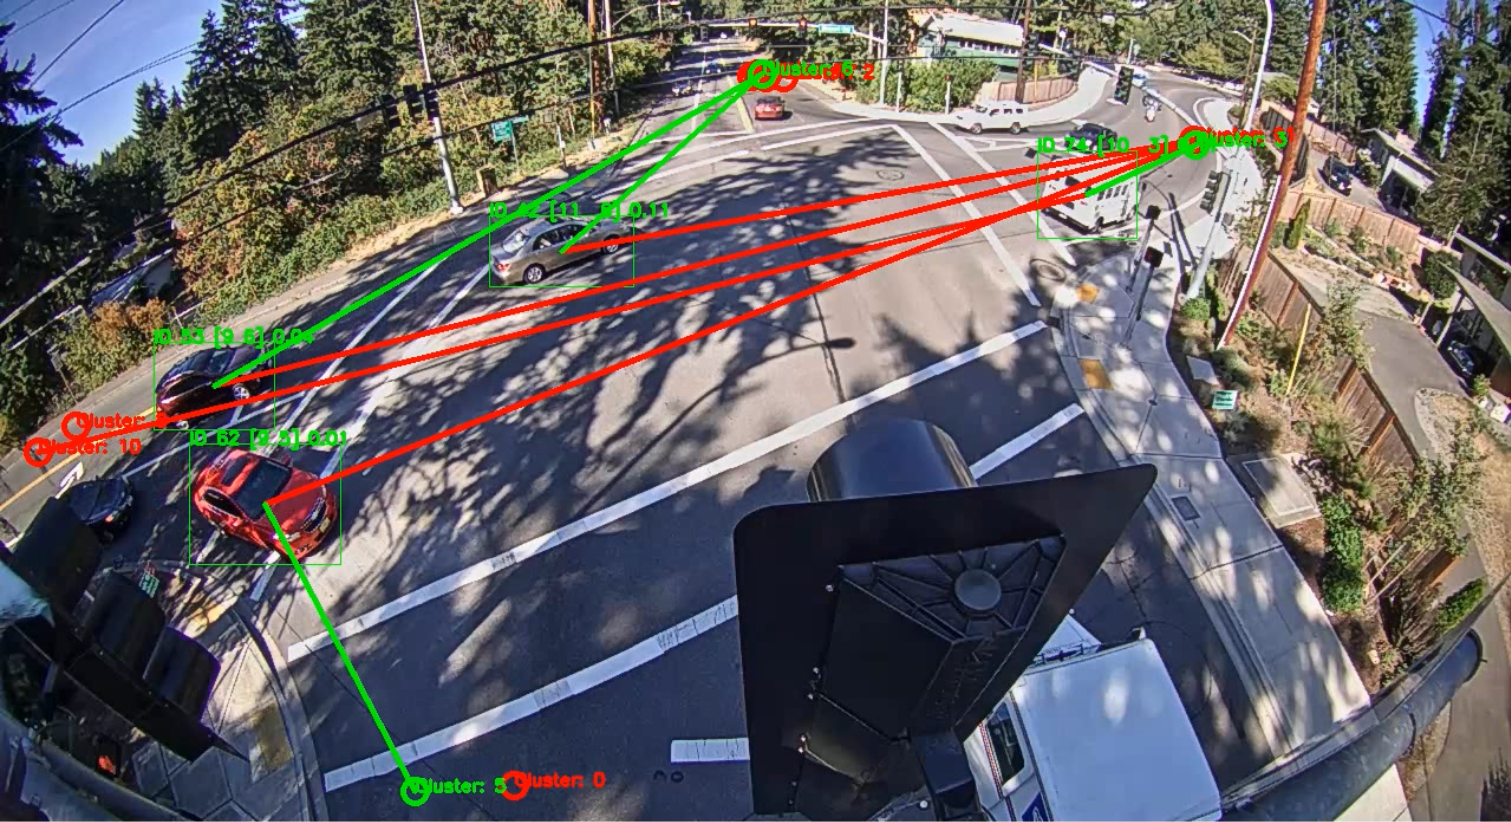
\includegraphics[width=1\columnwidth]{visualization/bellevue_newport.png}
    \caption{Bellevue Newport real time application}
    \label{BellevueNewportRealTime}
\end{figure}

\begin{figure}[htbp]
    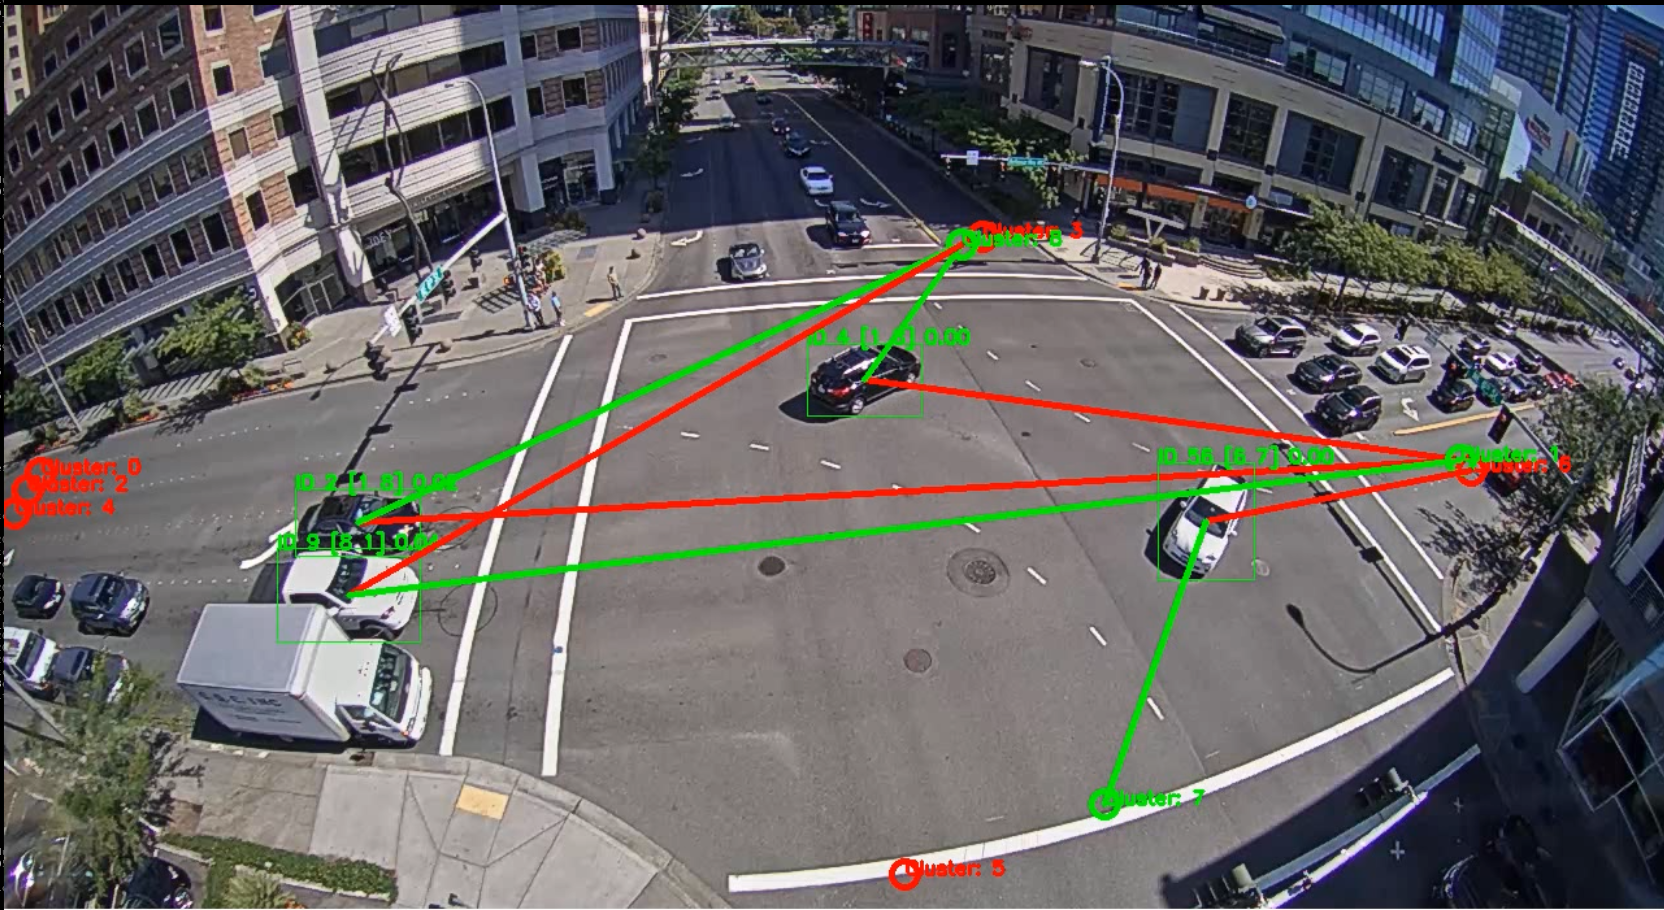
\includegraphics[width=1\columnwidth]{visualization/bellevue_ne.png}
    \caption{Bellevue NE real time application}
    \label{fig: BellevueNERealTime}
\end{figure}

\begin{figure}[htbp]
    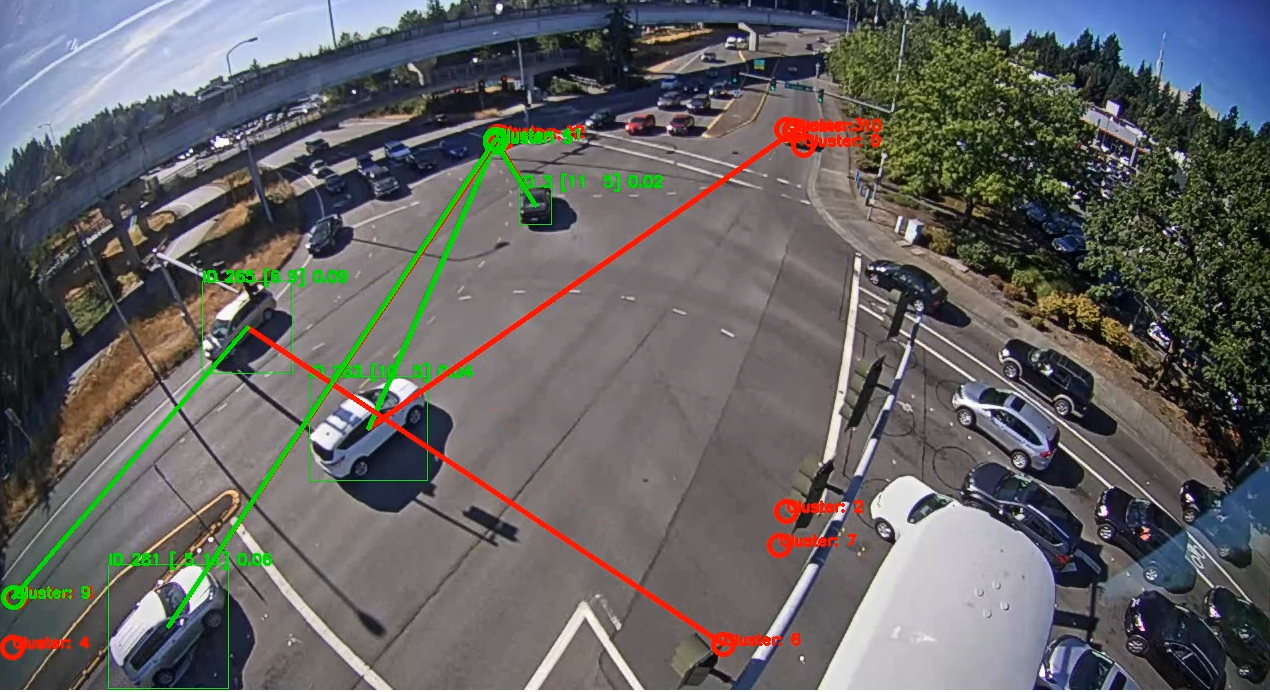
\includegraphics[width=1\columnwidth]{visualization/bellevue_eastgate.png}
    \caption{Bellevue Eastgate real time application}
    \label{fig: BellevueEastgateRealTime}
\end{figure}

\begin{figure}[htbp]
    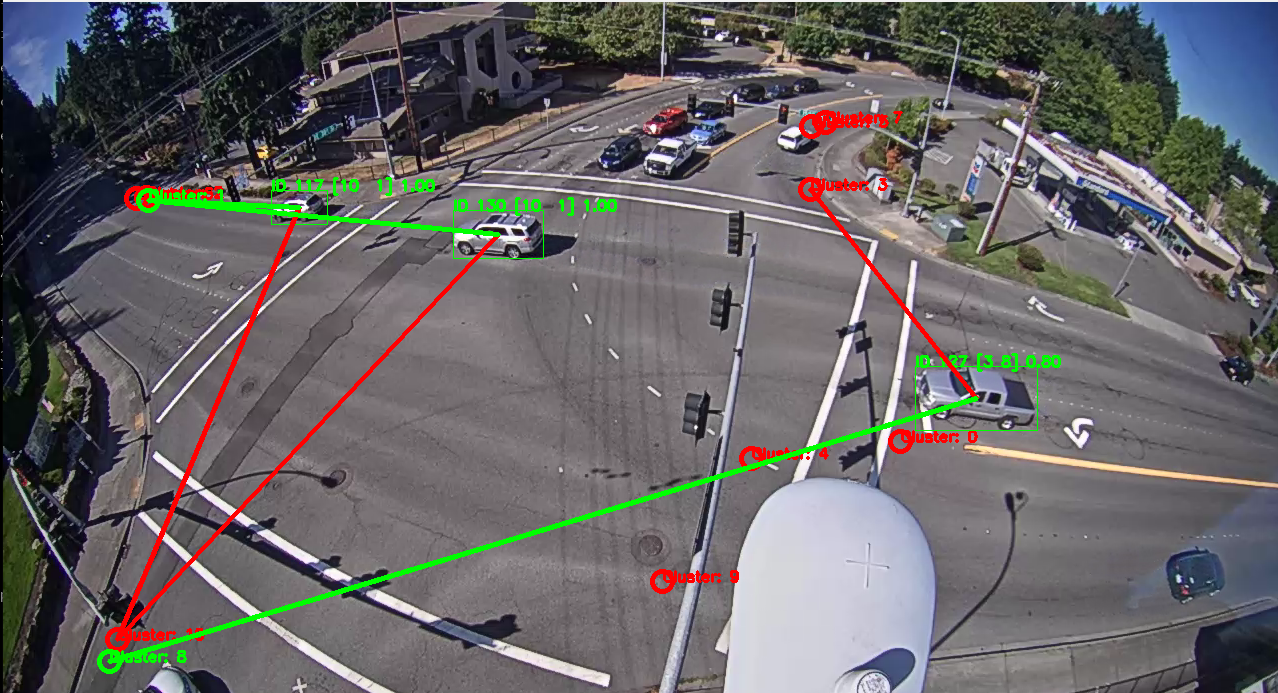
\includegraphics[width=1\columnwidth]{visualization/bellevue_se.png}
    \caption{Bellevue SE real time application}
    \label{fig: BellevueSERealTime}
\end{figure}

\newpage
\section{Forgalmi statisztikák}
%TODO itt lehetne egy kis bevezető, hogy miért fontosak a forgalmi statisztikák
A kidolgozott klaszterezési technikákkal kellő finomsággal tudjuk felosztani az útvonalakat, amik alapján statisztikai adatokat tudunk kinyerni.
A kinyert adatok alapján hiszotgramokat és hőtérképeket készítettünk. A hisztogramokon az egyes útvonalak teljes forgalmát tudjuk megjeleníteni,
a hőtérképeken pedig az egyes útvonalakon az autók óránkénti eloszlását. A hisztogramokat és hőtérképeket a \ref{fig:histogram} \ref{fig:histvisualisation} \ref{fig:heatmap} \ref{fig:heatmapnorm_cluster} \ref{fig:heatmapnorm_hourly} képeken lehet megtekinteni.
Forgalmi statisztikát generáló alkalmazásunkat részletesebben tárgyaljuk publikációnkban \cite{aggpeterhorvath2023}. %TODO cikk adatai: Folyoirat, datum, kozlesre elfogadva
%TODO sajat cikk megemlitese
\subsection{Hisztogram}
%TODO hisztogramok tárgyalása
A hisztogrammal az egyes csoportok teljes forgalmát tudjuk szemléltetni (lásd \ref{fig:histogram}). Hogy a hisztogramot könnyebb legyen értelmezni, a kereszteződés képére generáltuk az útvonalakat a hisztogram színeivel (lásd \ref{fig:heatmapnorm_cluster}).
%TODO ha lehet akkor csoportok osszevonas szerinti sorbarendezese
\begin{figure}[H]
    \centering
    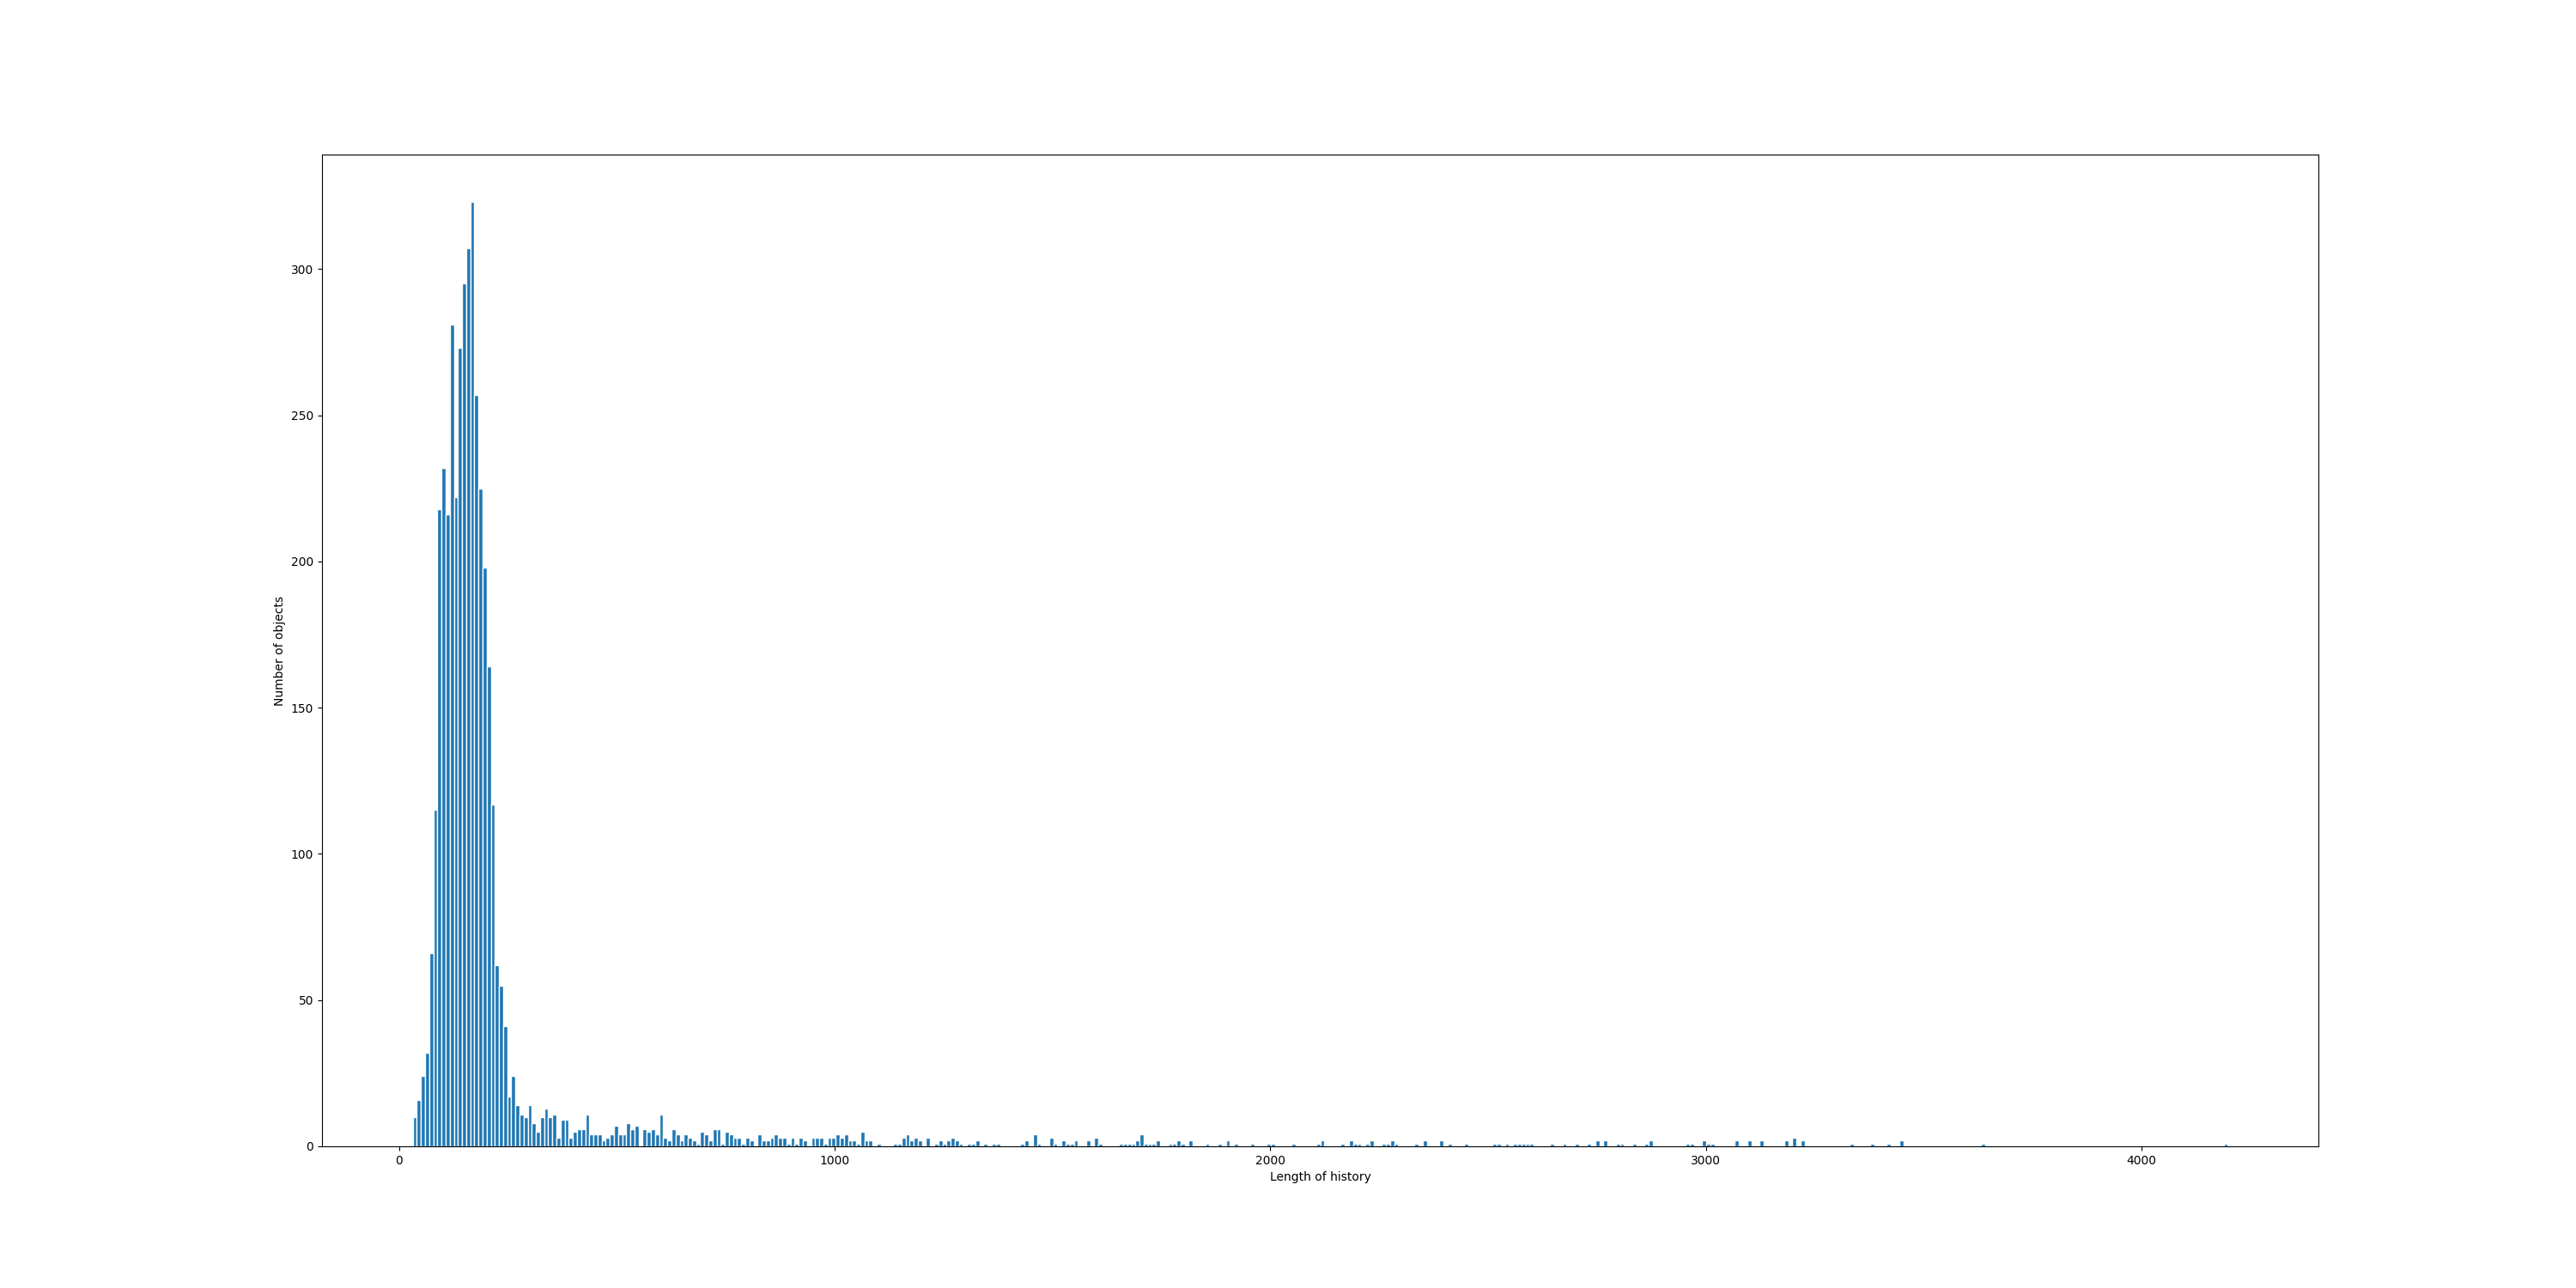
\includegraphics[width=1\columnwidth]{traffic_statistics/SE/histogram.png}
    \caption{Hisztogram}
    \label{fig:histogram}
\end{figure}
\begin{figure}[H]
    \centering
    \includegraphics[width=1\columnwidth]{traffic_statistics/SE/clusters.png}
    \caption{Hisztogram vizualizáció}
    \label{fig:histvisualisation}
\end{figure}
\subsection{Hőtérkép}
%TODO hőtérképek tárgyalása
Hőtérképen óránkénti és csoportonkénti felbontásban jelenítjük meg a járművek számát. A hőtérképeket a \ref{fig:heatmap} \ref{fig:heatmapnorm_cluster} \ref{fig:heatmapnorm_hourly} képeken lehet megtekinteni.
\subsubsection*{Abszólút értékes}
%TODO abszolút értékes hőtérkép magyarázat
Több fajta reprezentációt választottunk, az egyik az abszolút értékes megjelenítés, ahol az elhaladó járművek tényleges számát jelenítjük meg. Itt a színezés az összes órát és útvonalat figyelembe veszi (lásd \ref{fig:heatmap}).
\begin{figure}[H]
    \centering
    \includegraphics[width=1\columnwidth]{traffic_statistics/SE/heatmap_abs.png}
    \caption{Abszolút értékes hőtérkép}
    \label{fig:heatmap}
\end{figure}
\subsubsection*{Normalizált}
%TODO abszolút értékes hőtérkép magyarázat
A második reprezentációban a csoportonkénti normalizált értékeket jelenítjük meg, ahol az egyes csoportokban az óránkénti járművek számát normalizáljuk a csoporton belüli maximummal (lásd \ref{fig:heatmapnorm_cluster}).
\begin{figure}[H]
    \centering
    \includegraphics[width=1\columnwidth]{traffic_statistics/SE/heatmap_cluster_norm.png}
    \caption{Klaszterenként Normalizált hőtérkép}
    \label{fig:heatmapnorm_cluster}
\end{figure}
Az utolso verzióban az óránkénti normalizált értékeket jelenítjük meg, ahol az egyes csoportokban az óránkénti járművek számát normalizáljuk az óránkénti maximummal (lásd \ref{fig:heatmapnorm_hourly}).
\begin{figure}[H]
    \centering
    \includegraphics[width=1\columnwidth]{traffic_statistics/SE/heatmap_hourly_norm.png}
    \caption{Óránként Normalizált hőtérkép}
    \label{fig:heatmapnorm_hourly}
\end{figure}

\newpage
\section{Konklúzió}
\paragraph{A kiépített keretrendszer} a klaszterezéssel és klasszifikációs modellek betanításával egy fontos lépés ezen terület fejlesztésében.
Az adathalmazok előállítására kifejlesztett algoritmus hatékonynak bizonyult. Az adathalmaz feldolgozásához készített programokkal egy hatékony
adatfeldolgozó rendszert hoztunk létre. A klaszterezési algoritmusokkal a forgalomban előforduló útvonalakat sikerült megfelelően felosztani.
A kialakított tanítási folyamatnak köszönhetően a klasszifikációs modellek betanítása gyorsan és hatékonyan történik, a tanítás könnyen paraméterezhető, ami a további kísérletezésnél és modellek finomhangolásánál előnyt jelent.
A tanítás utáni kiértékelési fázishoz is készítettem programokat amikkel plotokat és táblázatokat tudunk generálni, amik az átláthatóságot javítják.
\paragraph{Grafikus megjelenítő} prototípus fejlesztésével a valós idejű alkalmazását lehet szemléltetni a kidolgozott módszerünknek. Továbbá jó alapul szolgál a jővőbeli praktikus felhasználáshoz.
\paragraph{A mérések} jó alapot szolgálnak a jövőbeli kutatásoknak, milyen algoritmusokat érdemes még mélyebben megvizsgálni és melyekkel nem érdemes a továbbiakban foglalkozni. Más objektumdetektáló és objektumkövető algoritmusokat is érdemes lehet kipróbálni, amiviel az adatgyűjtési fázist és az adattisztítási fázist lehet felgyorsítani és hatékonyabbá tenni.
\paragraph{Az átlagos 90\%} pontosság, amit elértünk a tanított modellekkel, nem tűnik túl magasnak, de figyelembe kell vennünk, hogy egy autó mozgása során sok olyan időszakasz van, amikor lehetetlen előre megmondani, melyik útvonalat fogja választani, mert pl. csak közelít a kereszteződéshez és nem választott még sávot. Ilyenkor az autó mozgása még semmilyen szinten nem utal a későbbi pályára, ezért óhatatlanul tévedések következnek be. A módszer predikciós képességét ilyenkor a ``top-2 accuracy" mutatja: a tipikusan 10-15 lehetséges útvonal-csoport közül a választott 2 legvalószínűbb már 95\% feletti eséllyel tartalmazza a ténylegesen bekövetkezőt.
\paragraph{Az adathalmaz növelésével} a pontosságot jövőben még növelni lehet. A feature vektorok dimenziószámának növelésével és másfajta súlyozással is növelhető ez a pontosság. A dimenzió növelése felveti a lehetőséget, hogy a jövőben mély neurális hálókat is teszteljünk az osztályozás feladatra.
\paragraph{A megerősító tanulás} bevezetése a keretrendszerünke is egy nagy előrelépés lehet, ezt úgy lehetne megvalósítani, hogy valós idejű futás közben, a bejövő adatokon nem csak osztályozást végzünk hanem ezeket az adatokat folyamatosan mentjük, majd ha elég adat összegyűlt időközönként frissítjük a modellt, így a modell adaptálódni tud a forgalom változásához.
\paragraph{A predikciós eljárásokon túl} a statisztikai kimutatások hasznos információként szolgálhatnak a forgalom megértéséhez, és a városi közlekedés optimalizálásához. Ezeket a kimutatásokat legfőképp közlekedés mérnökök tudják felhasználni.
%\section{Alkalmazási területek}

\newpage
\printbibliography
\end{document}